\documentclass[11pt]{article}
\usepackage[a4paper,margin=2.5cm]{geometry}
\usepackage{times}
\usepackage[authoryear,round]{natbib}
\usepackage{url}
\usepackage[T1]{fontenc}
\usepackage{amsmath,amssymb,amsthm}
\usepackage{booktabs}
\usepackage{graphicx}
\usepackage{xcolor}
\usepackage{algorithm}
\usepackage[noend]{algpseudocode}
\usepackage{tikz}
\usetikzlibrary{positioning,calc,arrows.meta,fit,backgrounds,shapes.geometric}
\usepackage[section]{placeins}
\usepackage[hidelinks]{hyperref}

\setlength{\emergencystretch}{2em}
\renewcommand{\topfraction}{0.9}
\renewcommand{\bottomfraction}{0.8}
\renewcommand{\textfraction}{0.07}
\renewcommand{\floatpagefraction}{0.8}
\setcounter{topnumber}{3}
\setcounter{bottomnumber}{2}
\setcounter{totalnumber}{5}
\newtheorem{proposition}{Proposition}
\newtheorem{corollary}{Corollary}
\theoremstyle{definition}
\newtheorem{definition}{Definition}
\theoremstyle{remark}
\newtheorem{remark}{Remark}
\newcommand{\E}{\mathbb{E}}
\algrenewcommand\algorithmicrequire{\textbf{Input:}}
\algrenewcommand\algorithmicensure{\textbf{Output:}}
\definecolor{cblue}{HTML}{2A78D6}
\definecolor{cblueL}{HTML}{CDE2FB}
\definecolor{corange}{HTML}{EB6834}
\definecolor{corangeL}{HTML}{FBE0D4}
\definecolor{cgreenL}{HTML}{D3F0E4}
\definecolor{cgray}{HTML}{F0EFEC}
\definecolor{lblue}{HTML}{2A78D6}
\definecolor{lorange}{HTML}{EB6834}

% every number comes from a result file; a missing key is an error, not a silently empty number
% generated by scripts/combined_assets.py -- do not edit
\expandafter\def\csname res@A-H1-CEC2022-ci\endcsname{[0.434, 0.489]}
\expandafter\def\csname res@A-H1-CEC2022-i1-amed\endcsname{2.43{\times}10^{-7}}
\expandafter\def\csname res@A-H1-CEC2022-i1-cmed\endcsname{1.59{\times}10^{-7}}
\expandafter\def\csname res@A-H1-CEC2022-i1-w\endcsname{0.36}
\expandafter\def\csname res@A-H1-CEC2022-i10-amed\endcsname{100.4}
\expandafter\def\csname res@A-H1-CEC2022-i10-cmed\endcsname{100.4}
\expandafter\def\csname res@A-H1-CEC2022-i10-w\endcsname{0.52}
\expandafter\def\csname res@A-H1-CEC2022-i11-amed\endcsname{300}
\expandafter\def\csname res@A-H1-CEC2022-i11-cmed\endcsname{300}
\expandafter\def\csname res@A-H1-CEC2022-i11-w\endcsname{0.54}
\expandafter\def\csname res@A-H1-CEC2022-i12-amed\endcsname{240.1}
\expandafter\def\csname res@A-H1-CEC2022-i12-cmed\endcsname{240.8}
\expandafter\def\csname res@A-H1-CEC2022-i12-w\endcsname{0.49}
\expandafter\def\csname res@A-H1-CEC2022-i2-amed\endcsname{44.9}
\expandafter\def\csname res@A-H1-CEC2022-i2-cmed\endcsname{49.08}
\expandafter\def\csname res@A-H1-CEC2022-i2-w\endcsname{0.43}
\expandafter\def\csname res@A-H1-CEC2022-i3-amed\endcsname{1.63{\times}10^{-5}}
\expandafter\def\csname res@A-H1-CEC2022-i3-cmed\endcsname{4.39{\times}10^{-6}}
\expandafter\def\csname res@A-H1-CEC2022-i3-w\endcsname{0.21}
\expandafter\def\csname res@A-H1-CEC2022-i4-amed\endcsname{37.31}
\expandafter\def\csname res@A-H1-CEC2022-i4-cmed\endcsname{33.83}
\expandafter\def\csname res@A-H1-CEC2022-i4-w\endcsname{0.38}
\expandafter\def\csname res@A-H1-CEC2022-i5-amed\endcsname{17.67}
\expandafter\def\csname res@A-H1-CEC2022-i5-cmed\endcsname{17.04}
\expandafter\def\csname res@A-H1-CEC2022-i5-w\endcsname{0.54}
\expandafter\def\csname res@A-H1-CEC2022-i6-amed\endcsname{20.02}
\expandafter\def\csname res@A-H1-CEC2022-i6-cmed\endcsname{17.65}
\expandafter\def\csname res@A-H1-CEC2022-i6-w\endcsname{0.51}
\expandafter\def\csname res@A-H1-CEC2022-i7-amed\endcsname{30.1}
\expandafter\def\csname res@A-H1-CEC2022-i7-cmed\endcsname{29.92}
\expandafter\def\csname res@A-H1-CEC2022-i7-w\endcsname{0.47}
\expandafter\def\csname res@A-H1-CEC2022-i8-amed\endcsname{20.96}
\expandafter\def\csname res@A-H1-CEC2022-i8-cmed\endcsname{21.01}
\expandafter\def\csname res@A-H1-CEC2022-i8-w\endcsname{0.46}
\expandafter\def\csname res@A-H1-CEC2022-i9-amed\endcsname{180.8}
\expandafter\def\csname res@A-H1-CEC2022-i9-cmed\endcsname{180.8}
\expandafter\def\csname res@A-H1-CEC2022-i9-w\endcsname{0.62}
\expandafter\def\csname res@A-H1-CEC2022-n\endcsname{12}
\expandafter\def\csname res@A-H1-CEC2022-rel\endcsname{-4.3{\times}10^{-4}}
\expandafter\def\csname res@A-H1-CEC2022-relmax\endcsname{2.4{\times}10^{0}}
\expandafter\def\csname res@A-H1-CEC2022-siga\endcsname{0}
\expandafter\def\csname res@A-H1-CEC2022-sigc\endcsname{1}
\expandafter\def\csname res@A-H1-CEC2022-verdict\endcsname{comparator superior}
\expandafter\def\csname res@A-H1-CEC2022-wbar\endcsname{0.461}
\expandafter\def\csname res@A-H1-FIR-ci\endcsname{[0.409, 0.476]}
\expandafter\def\csname res@A-H1-FIR-i1-amed\endcsname{5.17{\times}10^{-3}}
\expandafter\def\csname res@A-H1-FIR-i1-cmed\endcsname{4.81{\times}10^{-3}}
\expandafter\def\csname res@A-H1-FIR-i1-w\endcsname{0.28}
\expandafter\def\csname res@A-H1-FIR-i2-amed\endcsname{0.02158}
\expandafter\def\csname res@A-H1-FIR-i2-cmed\endcsname{0.02137}
\expandafter\def\csname res@A-H1-FIR-i2-w\endcsname{0.47}
\expandafter\def\csname res@A-H1-FIR-i3-amed\endcsname{5.09{\times}10^{-3}}
\expandafter\def\csname res@A-H1-FIR-i3-cmed\endcsname{4.82{\times}10^{-3}}
\expandafter\def\csname res@A-H1-FIR-i3-w\endcsname{0.39}
\expandafter\def\csname res@A-H1-FIR-i4-amed\endcsname{0.02151}
\expandafter\def\csname res@A-H1-FIR-i4-cmed\endcsname{0.02124}
\expandafter\def\csname res@A-H1-FIR-i4-w\endcsname{0.51}
\expandafter\def\csname res@A-H1-FIR-i5-amed\endcsname{1.74{\times}10^{-3}}
\expandafter\def\csname res@A-H1-FIR-i5-cmed\endcsname{1.41{\times}10^{-3}}
\expandafter\def\csname res@A-H1-FIR-i5-w\endcsname{0.36}
\expandafter\def\csname res@A-H1-FIR-i6-amed\endcsname{8.34{\times}10^{-3}}
\expandafter\def\csname res@A-H1-FIR-i6-cmed\endcsname{6.77{\times}10^{-3}}
\expandafter\def\csname res@A-H1-FIR-i6-w\endcsname{0.47}
\expandafter\def\csname res@A-H1-FIR-i7-amed\endcsname{1.32{\times}10^{-3}}
\expandafter\def\csname res@A-H1-FIR-i7-cmed\endcsname{1.60{\times}10^{-3}}
\expandafter\def\csname res@A-H1-FIR-i7-w\endcsname{0.52}
\expandafter\def\csname res@A-H1-FIR-i8-amed\endcsname{3.69{\times}10^{-3}}
\expandafter\def\csname res@A-H1-FIR-i8-cmed\endcsname{3.81{\times}10^{-3}}
\expandafter\def\csname res@A-H1-FIR-i8-w\endcsname{0.54}
\expandafter\def\csname res@A-H1-FIR-n\endcsname{8}
\expandafter\def\csname res@A-H1-FIR-rel\endcsname{-1.1{\times}10^{-2}}
\expandafter\def\csname res@A-H1-FIR-relmax\endcsname{1.4{\times}10^{-1}}
\expandafter\def\csname res@A-H1-FIR-siga\endcsname{0}
\expandafter\def\csname res@A-H1-FIR-sigc\endcsname{1}
\expandafter\def\csname res@A-H1-FIR-verdict\endcsname{comparator superior}
\expandafter\def\csname res@A-H1-FIR-wbar\endcsname{0.443}
\expandafter\def\csname res@A-H2a-CEC2022-ci\endcsname{[0.495, 0.573]}
\expandafter\def\csname res@A-H2a-CEC2022-i1-amed\endcsname{6.25{\times}10^{-13}}
\expandafter\def\csname res@A-H2a-CEC2022-i1-cmed\endcsname{3.98{\times}10^{-13}}
\expandafter\def\csname res@A-H2a-CEC2022-i1-w\endcsname{0.44}
\expandafter\def\csname res@A-H2a-CEC2022-i10-amed\endcsname{137.2}
\expandafter\def\csname res@A-H2a-CEC2022-i10-cmed\endcsname{101.5}
\expandafter\def\csname res@A-H2a-CEC2022-i10-w\endcsname{0.42}
\expandafter\def\csname res@A-H2a-CEC2022-i11-amed\endcsname{300}
\expandafter\def\csname res@A-H2a-CEC2022-i11-cmed\endcsname{300}
\expandafter\def\csname res@A-H2a-CEC2022-i11-w\endcsname{0.59}
\expandafter\def\csname res@A-H2a-CEC2022-i12-amed\endcsname{251.5}
\expandafter\def\csname res@A-H2a-CEC2022-i12-cmed\endcsname{251.7}
\expandafter\def\csname res@A-H2a-CEC2022-i12-w\endcsname{0.49}
\expandafter\def\csname res@A-H2a-CEC2022-i2-amed\endcsname{49.08}
\expandafter\def\csname res@A-H2a-CEC2022-i2-cmed\endcsname{46.99}
\expandafter\def\csname res@A-H2a-CEC2022-i2-w\endcsname{0.57}
\expandafter\def\csname res@A-H2a-CEC2022-i3-amed\endcsname{0.5583}
\expandafter\def\csname res@A-H2a-CEC2022-i3-cmed\endcsname{0.5669}
\expandafter\def\csname res@A-H2a-CEC2022-i3-w\endcsname{0.60}
\expandafter\def\csname res@A-H2a-CEC2022-i4-amed\endcsname{38.8}
\expandafter\def\csname res@A-H2a-CEC2022-i4-cmed\endcsname{45.77}
\expandafter\def\csname res@A-H2a-CEC2022-i4-w\endcsname{0.62}
\expandafter\def\csname res@A-H2a-CEC2022-i5-amed\endcsname{417.6}
\expandafter\def\csname res@A-H2a-CEC2022-i5-cmed\endcsname{330.8}
\expandafter\def\csname res@A-H2a-CEC2022-i5-w\endcsname{0.40}
\expandafter\def\csname res@A-H2a-CEC2022-i6-amed\endcsname{39.17}
\expandafter\def\csname res@A-H2a-CEC2022-i6-cmed\endcsname{45.1}
\expandafter\def\csname res@A-H2a-CEC2022-i6-w\endcsname{0.62}
\expandafter\def\csname res@A-H2a-CEC2022-i7-amed\endcsname{57.09}
\expandafter\def\csname res@A-H2a-CEC2022-i7-cmed\endcsname{56.02}
\expandafter\def\csname res@A-H2a-CEC2022-i7-w\endcsname{0.56}
\expandafter\def\csname res@A-H2a-CEC2022-i8-amed\endcsname{22.77}
\expandafter\def\csname res@A-H2a-CEC2022-i8-cmed\endcsname{22.92}
\expandafter\def\csname res@A-H2a-CEC2022-i8-w\endcsname{0.42}
\expandafter\def\csname res@A-H2a-CEC2022-i9-amed\endcsname{180.8}
\expandafter\def\csname res@A-H2a-CEC2022-i9-cmed\endcsname{180.8}
\expandafter\def\csname res@A-H2a-CEC2022-i9-w\endcsname{0.68}
\expandafter\def\csname res@A-H2a-CEC2022-n\endcsname{12}
\expandafter\def\csname res@A-H2a-CEC2022-rel\endcsname{6.3{\times}10^{-12}}
\expandafter\def\csname res@A-H2a-CEC2022-relmax\endcsname{1.0{\times}10^{0}}
\expandafter\def\csname res@A-H2a-CEC2022-siga\endcsname{0}
\expandafter\def\csname res@A-H2a-CEC2022-sigc\endcsname{0}
\expandafter\def\csname res@A-H2a-CEC2022-verdict\endcsname{inconclusive}
\expandafter\def\csname res@A-H2a-CEC2022-wbar\endcsname{0.534}
\expandafter\def\csname res@A-H2a-FIR-ci\endcsname{[0.527, 0.623]}
\expandafter\def\csname res@A-H2a-FIR-i1-amed\endcsname{4.85{\times}10^{-3}}
\expandafter\def\csname res@A-H2a-FIR-i1-cmed\endcsname{4.92{\times}10^{-3}}
\expandafter\def\csname res@A-H2a-FIR-i1-w\endcsname{0.56}
\expandafter\def\csname res@A-H2a-FIR-i2-amed\endcsname{0.02128}
\expandafter\def\csname res@A-H2a-FIR-i2-cmed\endcsname{0.02121}
\expandafter\def\csname res@A-H2a-FIR-i2-w\endcsname{0.46}
\expandafter\def\csname res@A-H2a-FIR-i3-amed\endcsname{4.81{\times}10^{-3}}
\expandafter\def\csname res@A-H2a-FIR-i3-cmed\endcsname{5.13{\times}10^{-3}}
\expandafter\def\csname res@A-H2a-FIR-i3-w\endcsname{0.58}
\expandafter\def\csname res@A-H2a-FIR-i4-amed\endcsname{0.02136}
\expandafter\def\csname res@A-H2a-FIR-i4-cmed\endcsname{0.022}
\expandafter\def\csname res@A-H2a-FIR-i4-w\endcsname{0.60}
\expandafter\def\csname res@A-H2a-FIR-i5-amed\endcsname{1.35{\times}10^{-3}}
\expandafter\def\csname res@A-H2a-FIR-i5-cmed\endcsname{2.04{\times}10^{-3}}
\expandafter\def\csname res@A-H2a-FIR-i5-w\endcsname{0.68}
\expandafter\def\csname res@A-H2a-FIR-i6-amed\endcsname{7.53{\times}10^{-3}}
\expandafter\def\csname res@A-H2a-FIR-i6-cmed\endcsname{7.29{\times}10^{-3}}
\expandafter\def\csname res@A-H2a-FIR-i6-w\endcsname{0.52}
\expandafter\def\csname res@A-H2a-FIR-i7-amed\endcsname{1.66{\times}10^{-3}}
\expandafter\def\csname res@A-H2a-FIR-i7-cmed\endcsname{1.88{\times}10^{-3}}
\expandafter\def\csname res@A-H2a-FIR-i7-w\endcsname{0.62}
\expandafter\def\csname res@A-H2a-FIR-i8-amed\endcsname{3.64{\times}10^{-3}}
\expandafter\def\csname res@A-H2a-FIR-i8-cmed\endcsname{3.98{\times}10^{-3}}
\expandafter\def\csname res@A-H2a-FIR-i8-w\endcsname{0.58}
\expandafter\def\csname res@A-H2a-FIR-n\endcsname{8}
\expandafter\def\csname res@A-H2a-FIR-rel\endcsname{1.4{\times}10^{-2}}
\expandafter\def\csname res@A-H2a-FIR-relmax\endcsname{1.6{\times}10^{-1}}
\expandafter\def\csname res@A-H2a-FIR-siga\endcsname{1}
\expandafter\def\csname res@A-H2a-FIR-sigc\endcsname{0}
\expandafter\def\csname res@A-H2a-FIR-verdict\endcsname{anchor superior}
\expandafter\def\csname res@A-H2a-FIR-wbar\endcsname{0.575}
\expandafter\def\csname res@A-H2b-CEC2022-ci\endcsname{[0.690, 0.743]}
\expandafter\def\csname res@A-H2b-CEC2022-i1-amed\endcsname{2.33{\times}10^{-7}}
\expandafter\def\csname res@A-H2b-CEC2022-i1-cmed\endcsname{6.25{\times}10^{-13}}
\expandafter\def\csname res@A-H2b-CEC2022-i1-w\endcsname{0.12}
\expandafter\def\csname res@A-H2b-CEC2022-i10-amed\endcsname{100.4}
\expandafter\def\csname res@A-H2b-CEC2022-i10-cmed\endcsname{137.2}
\expandafter\def\csname res@A-H2b-CEC2022-i10-w\endcsname{0.92}
\expandafter\def\csname res@A-H2b-CEC2022-i11-amed\endcsname{300}
\expandafter\def\csname res@A-H2b-CEC2022-i11-cmed\endcsname{300}
\expandafter\def\csname res@A-H2b-CEC2022-i11-w\endcsname{0.18}
\expandafter\def\csname res@A-H2b-CEC2022-i12-amed\endcsname{241.6}
\expandafter\def\csname res@A-H2b-CEC2022-i12-cmed\endcsname{251.5}
\expandafter\def\csname res@A-H2b-CEC2022-i12-w\endcsname{0.92}
\expandafter\def\csname res@A-H2b-CEC2022-i2-amed\endcsname{49.08}
\expandafter\def\csname res@A-H2b-CEC2022-i2-cmed\endcsname{49.08}
\expandafter\def\csname res@A-H2b-CEC2022-i2-w\endcsname{0.36}
\expandafter\def\csname res@A-H2b-CEC2022-i3-amed\endcsname{4.01{\times}10^{-6}}
\expandafter\def\csname res@A-H2b-CEC2022-i3-cmed\endcsname{0.5583}
\expandafter\def\csname res@A-H2b-CEC2022-i3-w\endcsname{1.00}
\expandafter\def\csname res@A-H2b-CEC2022-i4-amed\endcsname{29.85}
\expandafter\def\csname res@A-H2b-CEC2022-i4-cmed\endcsname{38.8}
\expandafter\def\csname res@A-H2b-CEC2022-i4-w\endcsname{0.72}
\expandafter\def\csname res@A-H2b-CEC2022-i5-amed\endcsname{16.53}
\expandafter\def\csname res@A-H2b-CEC2022-i5-cmed\endcsname{417.6}
\expandafter\def\csname res@A-H2b-CEC2022-i5-w\endcsname{1.00}
\expandafter\def\csname res@A-H2b-CEC2022-i6-amed\endcsname{16.05}
\expandafter\def\csname res@A-H2b-CEC2022-i6-cmed\endcsname{39.17}
\expandafter\def\csname res@A-H2b-CEC2022-i6-w\endcsname{0.82}
\expandafter\def\csname res@A-H2b-CEC2022-i7-amed\endcsname{31.1}
\expandafter\def\csname res@A-H2b-CEC2022-i7-cmed\endcsname{57.09}
\expandafter\def\csname res@A-H2b-CEC2022-i7-w\endcsname{0.86}
\expandafter\def\csname res@A-H2b-CEC2022-i8-amed\endcsname{21.09}
\expandafter\def\csname res@A-H2b-CEC2022-i8-cmed\endcsname{22.77}
\expandafter\def\csname res@A-H2b-CEC2022-i8-w\endcsname{0.94}
\expandafter\def\csname res@A-H2b-CEC2022-i9-amed\endcsname{180.8}
\expandafter\def\csname res@A-H2b-CEC2022-i9-cmed\endcsname{180.8}
\expandafter\def\csname res@A-H2b-CEC2022-i9-w\endcsname{0.76}
\expandafter\def\csname res@A-H2b-CEC2022-n\endcsname{12}
\expandafter\def\csname res@A-H2b-CEC2022-rel\endcsname{1.9{\times}10^{-1}}
\expandafter\def\csname res@A-H2b-CEC2022-relmax\endcsname{2.3{\times}10^{5}}
\expandafter\def\csname res@A-H2b-CEC2022-siga\endcsname{9}
\expandafter\def\csname res@A-H2b-CEC2022-sigc\endcsname{2}
\expandafter\def\csname res@A-H2b-CEC2022-verdict\endcsname{mixed}
\expandafter\def\csname res@A-H2b-CEC2022-wbar\endcsname{0.717}
\expandafter\def\csname res@A-H3-CEC2022-ci\endcsname{[0.545, 0.613]}
\expandafter\def\csname res@A-H3-CEC2022-i1-amed\endcsname{2.49{\times}10^{-7}}
\expandafter\def\csname res@A-H3-CEC2022-i1-cmed\endcsname{2.05{\times}10^{-4}}
\expandafter\def\csname res@A-H3-CEC2022-i1-w\endcsname{1.00}
\expandafter\def\csname res@A-H3-CEC2022-i10-amed\endcsname{100.4}
\expandafter\def\csname res@A-H3-CEC2022-i10-cmed\endcsname{100.5}
\expandafter\def\csname res@A-H3-CEC2022-i10-w\endcsname{0.68}
\expandafter\def\csname res@A-H3-CEC2022-i11-amed\endcsname{300}
\expandafter\def\csname res@A-H3-CEC2022-i11-cmed\endcsname{300}
\expandafter\def\csname res@A-H3-CEC2022-i11-w\endcsname{0.38}
\expandafter\def\csname res@A-H3-CEC2022-i12-amed\endcsname{240.6}
\expandafter\def\csname res@A-H3-CEC2022-i12-cmed\endcsname{239.5}
\expandafter\def\csname res@A-H3-CEC2022-i12-w\endcsname{0.44}
\expandafter\def\csname res@A-H3-CEC2022-i2-amed\endcsname{49.08}
\expandafter\def\csname res@A-H3-CEC2022-i2-cmed\endcsname{44.9}
\expandafter\def\csname res@A-H3-CEC2022-i2-w\endcsname{0.56}
\expandafter\def\csname res@A-H3-CEC2022-i3-amed\endcsname{1.39{\times}10^{-5}}
\expandafter\def\csname res@A-H3-CEC2022-i3-cmed\endcsname{0.01421}
\expandafter\def\csname res@A-H3-CEC2022-i3-w\endcsname{1.00}
\expandafter\def\csname res@A-H3-CEC2022-i4-amed\endcsname{36.32}
\expandafter\def\csname res@A-H3-CEC2022-i4-cmed\endcsname{37.31}
\expandafter\def\csname res@A-H3-CEC2022-i4-w\endcsname{0.40}
\expandafter\def\csname res@A-H3-CEC2022-i5-amed\endcsname{20.84}
\expandafter\def\csname res@A-H3-CEC2022-i5-cmed\endcsname{13.29}
\expandafter\def\csname res@A-H3-CEC2022-i5-w\endcsname{0.30}
\expandafter\def\csname res@A-H3-CEC2022-i6-amed\endcsname{20.02}
\expandafter\def\csname res@A-H3-CEC2022-i6-cmed\endcsname{12.2}
\expandafter\def\csname res@A-H3-CEC2022-i6-w\endcsname{0.34}
\expandafter\def\csname res@A-H3-CEC2022-i7-amed\endcsname{32.93}
\expandafter\def\csname res@A-H3-CEC2022-i7-cmed\endcsname{26.62}
\expandafter\def\csname res@A-H3-CEC2022-i7-w\endcsname{0.34}
\expandafter\def\csname res@A-H3-CEC2022-i8-amed\endcsname{20.92}
\expandafter\def\csname res@A-H3-CEC2022-i8-cmed\endcsname{21.09}
\expandafter\def\csname res@A-H3-CEC2022-i8-w\endcsname{0.64}
\expandafter\def\csname res@A-H3-CEC2022-i9-amed\endcsname{180.8}
\expandafter\def\csname res@A-H3-CEC2022-i9-cmed\endcsname{180.8}
\expandafter\def\csname res@A-H3-CEC2022-i9-w\endcsname{0.87}
\expandafter\def\csname res@A-H3-CEC2022-n\endcsname{12}
\expandafter\def\csname res@A-H3-CEC2022-rel\endcsname{1.0{\times}10^{-9}}
\expandafter\def\csname res@A-H3-CEC2022-relmax\endcsname{1.0{\times}10^{0}}
\expandafter\def\csname res@A-H3-CEC2022-siga\endcsname{4}
\expandafter\def\csname res@A-H3-CEC2022-sigc\endcsname{2}
\expandafter\def\csname res@A-H3-CEC2022-verdict\endcsname{mixed}
\expandafter\def\csname res@A-H3-CEC2022-wbar\endcsname{0.579}
\expandafter\def\csname res@A-H3-FIR-ci\endcsname{[0.943, 0.980]}
\expandafter\def\csname res@A-H3-FIR-i1-amed\endcsname{5.06{\times}10^{-3}}
\expandafter\def\csname res@A-H3-FIR-i1-cmed\endcsname{0.0123}
\expandafter\def\csname res@A-H3-FIR-i1-w\endcsname{0.98}
\expandafter\def\csname res@A-H3-FIR-i2-amed\endcsname{0.0221}
\expandafter\def\csname res@A-H3-FIR-i2-cmed\endcsname{0.03011}
\expandafter\def\csname res@A-H3-FIR-i2-w\endcsname{0.96}
\expandafter\def\csname res@A-H3-FIR-i3-amed\endcsname{5.13{\times}10^{-3}}
\expandafter\def\csname res@A-H3-FIR-i3-cmed\endcsname{0.01031}
\expandafter\def\csname res@A-H3-FIR-i3-w\endcsname{0.96}
\expandafter\def\csname res@A-H3-FIR-i4-amed\endcsname{0.02119}
\expandafter\def\csname res@A-H3-FIR-i4-cmed\endcsname{0.02994}
\expandafter\def\csname res@A-H3-FIR-i4-w\endcsname{1.00}
\expandafter\def\csname res@A-H3-FIR-i5-amed\endcsname{1.83{\times}10^{-3}}
\expandafter\def\csname res@A-H3-FIR-i5-cmed\endcsname{5.76{\times}10^{-3}}
\expandafter\def\csname res@A-H3-FIR-i5-w\endcsname{0.98}
\expandafter\def\csname res@A-H3-FIR-i6-amed\endcsname{7.95{\times}10^{-3}}
\expandafter\def\csname res@A-H3-FIR-i6-cmed\endcsname{0.01186}
\expandafter\def\csname res@A-H3-FIR-i6-w\endcsname{0.96}
\expandafter\def\csname res@A-H3-FIR-i7-amed\endcsname{1.16{\times}10^{-3}}
\expandafter\def\csname res@A-H3-FIR-i7-cmed\endcsname{6.42{\times}10^{-3}}
\expandafter\def\csname res@A-H3-FIR-i7-w\endcsname{1.00}
\expandafter\def\csname res@A-H3-FIR-i8-amed\endcsname{3.83{\times}10^{-3}}
\expandafter\def\csname res@A-H3-FIR-i8-cmed\endcsname{9.49{\times}10^{-3}}
\expandafter\def\csname res@A-H3-FIR-i8-w\endcsname{0.86}
\expandafter\def\csname res@A-H3-FIR-n\endcsname{8}
\expandafter\def\csname res@A-H3-FIR-rel\endcsname{5.4{\times}10^{-1}}
\expandafter\def\csname res@A-H3-FIR-relmax\endcsname{7.9{\times}10^{-1}}
\expandafter\def\csname res@A-H3-FIR-siga\endcsname{8}
\expandafter\def\csname res@A-H3-FIR-sigc\endcsname{0}
\expandafter\def\csname res@A-H3-FIR-verdict\endcsname{anchor superior}
\expandafter\def\csname res@A-H3-FIR-wbar\endcsname{0.962}
\expandafter\def\csname res@A-H4-CEC2022-ci\endcsname{[0.757, 0.802]}
\expandafter\def\csname res@A-H4-CEC2022-i1-amed\endcsname{2.05{\times}10^{-4}}
\expandafter\def\csname res@A-H4-CEC2022-i1-cmed\endcsname{2.05{\times}10^{-4}}
\expandafter\def\csname res@A-H4-CEC2022-i1-w\endcsname{0.91}
\expandafter\def\csname res@A-H4-CEC2022-i10-amed\endcsname{100.5}
\expandafter\def\csname res@A-H4-CEC2022-i10-cmed\endcsname{100.5}
\expandafter\def\csname res@A-H4-CEC2022-i10-w\endcsname{0.59}
\expandafter\def\csname res@A-H4-CEC2022-i11-amed\endcsname{300}
\expandafter\def\csname res@A-H4-CEC2022-i11-cmed\endcsname{300}
\expandafter\def\csname res@A-H4-CEC2022-i11-w\endcsname{0.69}
\expandafter\def\csname res@A-H4-CEC2022-i12-amed\endcsname{239.5}
\expandafter\def\csname res@A-H4-CEC2022-i12-cmed\endcsname{239.5}
\expandafter\def\csname res@A-H4-CEC2022-i12-w\endcsname{0.72}
\expandafter\def\csname res@A-H4-CEC2022-i2-amed\endcsname{44.9}
\expandafter\def\csname res@A-H4-CEC2022-i2-cmed\endcsname{44.9}
\expandafter\def\csname res@A-H4-CEC2022-i2-w\endcsname{0.82}
\expandafter\def\csname res@A-H4-CEC2022-i3-amed\endcsname{0.01421}
\expandafter\def\csname res@A-H4-CEC2022-i3-cmed\endcsname{0.01423}
\expandafter\def\csname res@A-H4-CEC2022-i3-w\endcsname{0.91}
\expandafter\def\csname res@A-H4-CEC2022-i4-amed\endcsname{37.31}
\expandafter\def\csname res@A-H4-CEC2022-i4-cmed\endcsname{37.31}
\expandafter\def\csname res@A-H4-CEC2022-i4-w\endcsname{0.85}
\expandafter\def\csname res@A-H4-CEC2022-i5-amed\endcsname{13.29}
\expandafter\def\csname res@A-H4-CEC2022-i5-cmed\endcsname{13.29}
\expandafter\def\csname res@A-H4-CEC2022-i5-w\endcsname{0.89}
\expandafter\def\csname res@A-H4-CEC2022-i6-amed\endcsname{12.2}
\expandafter\def\csname res@A-H4-CEC2022-i6-cmed\endcsname{12.2}
\expandafter\def\csname res@A-H4-CEC2022-i6-w\endcsname{0.86}
\expandafter\def\csname res@A-H4-CEC2022-i7-amed\endcsname{26.62}
\expandafter\def\csname res@A-H4-CEC2022-i7-cmed\endcsname{26.62}
\expandafter\def\csname res@A-H4-CEC2022-i7-w\endcsname{0.77}
\expandafter\def\csname res@A-H4-CEC2022-i8-amed\endcsname{21.09}
\expandafter\def\csname res@A-H4-CEC2022-i8-cmed\endcsname{21.09}
\expandafter\def\csname res@A-H4-CEC2022-i8-w\endcsname{0.64}
\expandafter\def\csname res@A-H4-CEC2022-i9-amed\endcsname{180.8}
\expandafter\def\csname res@A-H4-CEC2022-i9-cmed\endcsname{180.8}
\expandafter\def\csname res@A-H4-CEC2022-i9-w\endcsname{0.71}
\expandafter\def\csname res@A-H4-CEC2022-n\endcsname{12}
\expandafter\def\csname res@A-H4-CEC2022-rel\endcsname{6.4{\times}10^{-11}}
\expandafter\def\csname res@A-H4-CEC2022-relmax\endcsname{1.0{\times}10^{-4}}
\expandafter\def\csname res@A-H4-CEC2022-siga\endcsname{12}
\expandafter\def\csname res@A-H4-CEC2022-sigc\endcsname{0}
\expandafter\def\csname res@A-H4-CEC2022-verdict\endcsname{anchor superior}
\expandafter\def\csname res@A-H4-CEC2022-wbar\endcsname{0.780}
\expandafter\def\csname res@A-H4-FIR-ci\endcsname{[0.798, 0.853]}
\expandafter\def\csname res@A-H4-FIR-i1-amed\endcsname{0.0123}
\expandafter\def\csname res@A-H4-FIR-i1-cmed\endcsname{0.0123}
\expandafter\def\csname res@A-H4-FIR-i1-w\endcsname{0.90}
\expandafter\def\csname res@A-H4-FIR-i2-amed\endcsname{0.03011}
\expandafter\def\csname res@A-H4-FIR-i2-cmed\endcsname{0.03011}
\expandafter\def\csname res@A-H4-FIR-i2-w\endcsname{0.86}
\expandafter\def\csname res@A-H4-FIR-i3-amed\endcsname{0.01031}
\expandafter\def\csname res@A-H4-FIR-i3-cmed\endcsname{0.01031}
\expandafter\def\csname res@A-H4-FIR-i3-w\endcsname{0.82}
\expandafter\def\csname res@A-H4-FIR-i4-amed\endcsname{0.02994}
\expandafter\def\csname res@A-H4-FIR-i4-cmed\endcsname{0.02994}
\expandafter\def\csname res@A-H4-FIR-i4-w\endcsname{0.82}
\expandafter\def\csname res@A-H4-FIR-i5-amed\endcsname{5.76{\times}10^{-3}}
\expandafter\def\csname res@A-H4-FIR-i5-cmed\endcsname{5.76{\times}10^{-3}}
\expandafter\def\csname res@A-H4-FIR-i5-w\endcsname{0.74}
\expandafter\def\csname res@A-H4-FIR-i6-amed\endcsname{0.01186}
\expandafter\def\csname res@A-H4-FIR-i6-cmed\endcsname{0.01186}
\expandafter\def\csname res@A-H4-FIR-i6-w\endcsname{0.86}
\expandafter\def\csname res@A-H4-FIR-i7-amed\endcsname{6.42{\times}10^{-3}}
\expandafter\def\csname res@A-H4-FIR-i7-cmed\endcsname{6.42{\times}10^{-3}}
\expandafter\def\csname res@A-H4-FIR-i7-w\endcsname{0.79}
\expandafter\def\csname res@A-H4-FIR-i8-amed\endcsname{9.49{\times}10^{-3}}
\expandafter\def\csname res@A-H4-FIR-i8-cmed\endcsname{9.49{\times}10^{-3}}
\expandafter\def\csname res@A-H4-FIR-i8-w\endcsname{0.82}
\expandafter\def\csname res@A-H4-FIR-n\endcsname{8}
\expandafter\def\csname res@A-H4-FIR-rel\endcsname{1.3{\times}10^{-8}}
\expandafter\def\csname res@A-H4-FIR-relmax\endcsname{3.6{\times}10^{-8}}
\expandafter\def\csname res@A-H4-FIR-siga\endcsname{8}
\expandafter\def\csname res@A-H4-FIR-sigc\endcsname{0}
\expandafter\def\csname res@A-H4-FIR-verdict\endcsname{anchor superior}
\expandafter\def\csname res@A-H4-FIR-wbar\endcsname{0.826}
\expandafter\def\csname res@A-H5-RND-AUTH-ci\endcsname{[0.06, 0.17]}
\expandafter\def\csname res@A-H5-RND-AUTH-esc\endcsname{10}
\expandafter\def\csname res@A-H5-RND-AUTH-n\endcsname{100}
\expandafter\def\csname res@A-H5-RND-FAIR-ci\endcsname{[0.18, 0.34]}
\expandafter\def\csname res@A-H5-RND-FAIR-esc\endcsname{25}
\expandafter\def\csname res@A-H5-RND-FAIR-n\endcsname{100}
\expandafter\def\csname res@A-H5-SARSA-ci\endcsname{[0.18, 0.35]}
\expandafter\def\csname res@A-H5-SARSA-esc\endcsname{26}
\expandafter\def\csname res@A-H5-SARSA-n\endcsname{100}
\expandafter\def\csname res@A-H5-SKEL-ci\endcsname{[0.00, 0.04]}
\expandafter\def\csname res@A-H5-SKEL-esc\endcsname{0}
\expandafter\def\csname res@A-H5-SKEL-n\endcsname{100}
\expandafter\def\csname res@A-H5-binom-p\endcsname{7.7\times10^{-10}}
\expandafter\def\csname res@A-H5-mcnemar-p\endcsname{1.00}
\expandafter\def\csname res@A-H6-Ni1-policy-CEC2022-ci\endcsname{[0.427, 0.504]}
\expandafter\def\csname res@A-H6-Ni1-policy-CEC2022-i1-amed\endcsname{5.80{\times}10^{-7}}
\expandafter\def\csname res@A-H6-Ni1-policy-CEC2022-i1-cmed\endcsname{4.86{\times}10^{-7}}
\expandafter\def\csname res@A-H6-Ni1-policy-CEC2022-i1-w\endcsname{0.34}
\expandafter\def\csname res@A-H6-Ni1-policy-CEC2022-i10-amed\endcsname{100.5}
\expandafter\def\csname res@A-H6-Ni1-policy-CEC2022-i10-cmed\endcsname{100.5}
\expandafter\def\csname res@A-H6-Ni1-policy-CEC2022-i10-w\endcsname{0.46}
\expandafter\def\csname res@A-H6-Ni1-policy-CEC2022-i11-amed\endcsname{300}
\expandafter\def\csname res@A-H6-Ni1-policy-CEC2022-i11-cmed\endcsname{300}
\expandafter\def\csname res@A-H6-Ni1-policy-CEC2022-i11-w\endcsname{0.64}
\expandafter\def\csname res@A-H6-Ni1-policy-CEC2022-i12-amed\endcsname{240.2}
\expandafter\def\csname res@A-H6-Ni1-policy-CEC2022-i12-cmed\endcsname{237.6}
\expandafter\def\csname res@A-H6-Ni1-policy-CEC2022-i12-w\endcsname{0.40}
\expandafter\def\csname res@A-H6-Ni1-policy-CEC2022-i2-amed\endcsname{49.08}
\expandafter\def\csname res@A-H6-Ni1-policy-CEC2022-i2-cmed\endcsname{46.99}
\expandafter\def\csname res@A-H6-Ni1-policy-CEC2022-i2-w\endcsname{0.46}
\expandafter\def\csname res@A-H6-Ni1-policy-CEC2022-i3-amed\endcsname{4.11{\times}10^{-5}}
\expandafter\def\csname res@A-H6-Ni1-policy-CEC2022-i3-cmed\endcsname{2.31{\times}10^{-5}}
\expandafter\def\csname res@A-H6-Ni1-policy-CEC2022-i3-w\endcsname{0.34}
\expandafter\def\csname res@A-H6-Ni1-policy-CEC2022-i4-amed\endcsname{33.83}
\expandafter\def\csname res@A-H6-Ni1-policy-CEC2022-i4-cmed\endcsname{34.33}
\expandafter\def\csname res@A-H6-Ni1-policy-CEC2022-i4-w\endcsname{0.50}
\expandafter\def\csname res@A-H6-Ni1-policy-CEC2022-i5-amed\endcsname{10.11}
\expandafter\def\csname res@A-H6-Ni1-policy-CEC2022-i5-cmed\endcsname{10.77}
\expandafter\def\csname res@A-H6-Ni1-policy-CEC2022-i5-w\endcsname{0.54}
\expandafter\def\csname res@A-H6-Ni1-policy-CEC2022-i6-amed\endcsname{13.9}
\expandafter\def\csname res@A-H6-Ni1-policy-CEC2022-i6-cmed\endcsname{13.3}
\expandafter\def\csname res@A-H6-Ni1-policy-CEC2022-i6-w\endcsname{0.46}
\expandafter\def\csname res@A-H6-Ni1-policy-CEC2022-i7-amed\endcsname{25.98}
\expandafter\def\csname res@A-H6-Ni1-policy-CEC2022-i7-cmed\endcsname{25.97}
\expandafter\def\csname res@A-H6-Ni1-policy-CEC2022-i7-w\endcsname{0.46}
\expandafter\def\csname res@A-H6-Ni1-policy-CEC2022-i8-amed\endcsname{20.83}
\expandafter\def\csname res@A-H6-Ni1-policy-CEC2022-i8-cmed\endcsname{20.95}
\expandafter\def\csname res@A-H6-Ni1-policy-CEC2022-i8-w\endcsname{0.52}
\expandafter\def\csname res@A-H6-Ni1-policy-CEC2022-i9-amed\endcsname{180.8}
\expandafter\def\csname res@A-H6-Ni1-policy-CEC2022-i9-cmed\endcsname{180.8}
\expandafter\def\csname res@A-H6-Ni1-policy-CEC2022-i9-w\endcsname{0.46}
\expandafter\def\csname res@A-H6-Ni1-policy-CEC2022-n\endcsname{12}
\expandafter\def\csname res@A-H6-Ni1-policy-CEC2022-rel\endcsname{-7.9{\times}10^{-5}}
\expandafter\def\csname res@A-H6-Ni1-policy-CEC2022-relmax\endcsname{1.4{\times}10^{0}}
\expandafter\def\csname res@A-H6-Ni1-policy-CEC2022-siga\endcsname{0}
\expandafter\def\csname res@A-H6-Ni1-policy-CEC2022-sigc\endcsname{0}
\expandafter\def\csname res@A-H6-Ni1-policy-CEC2022-verdict\endcsname{inconclusive}
\expandafter\def\csname res@A-H6-Ni1-policy-CEC2022-wbar\endcsname{0.465}
\expandafter\def\csname res@A-H6-Ni1-policy-FIR-ci\endcsname{[0.422, 0.518]}
\expandafter\def\csname res@A-H6-Ni1-policy-FIR-i1-amed\endcsname{5.26{\times}10^{-3}}
\expandafter\def\csname res@A-H6-Ni1-policy-FIR-i1-cmed\endcsname{4.86{\times}10^{-3}}
\expandafter\def\csname res@A-H6-Ni1-policy-FIR-i1-w\endcsname{0.38}
\expandafter\def\csname res@A-H6-Ni1-policy-FIR-i2-amed\endcsname{0.02117}
\expandafter\def\csname res@A-H6-Ni1-policy-FIR-i2-cmed\endcsname{0.0219}
\expandafter\def\csname res@A-H6-Ni1-policy-FIR-i2-w\endcsname{0.58}
\expandafter\def\csname res@A-H6-Ni1-policy-FIR-i3-amed\endcsname{5.22{\times}10^{-3}}
\expandafter\def\csname res@A-H6-Ni1-policy-FIR-i3-cmed\endcsname{5.26{\times}10^{-3}}
\expandafter\def\csname res@A-H6-Ni1-policy-FIR-i3-w\endcsname{0.54}
\expandafter\def\csname res@A-H6-Ni1-policy-FIR-i4-amed\endcsname{0.02141}
\expandafter\def\csname res@A-H6-Ni1-policy-FIR-i4-cmed\endcsname{0.02132}
\expandafter\def\csname res@A-H6-Ni1-policy-FIR-i4-w\endcsname{0.54}
\expandafter\def\csname res@A-H6-Ni1-policy-FIR-i5-amed\endcsname{2.06{\times}10^{-3}}
\expandafter\def\csname res@A-H6-Ni1-policy-FIR-i5-cmed\endcsname{2.07{\times}10^{-3}}
\expandafter\def\csname res@A-H6-Ni1-policy-FIR-i5-w\endcsname{0.54}
\expandafter\def\csname res@A-H6-Ni1-policy-FIR-i6-amed\endcsname{8.36{\times}10^{-3}}
\expandafter\def\csname res@A-H6-Ni1-policy-FIR-i6-cmed\endcsname{8.34{\times}10^{-3}}
\expandafter\def\csname res@A-H6-Ni1-policy-FIR-i6-w\endcsname{0.42}
\expandafter\def\csname res@A-H6-Ni1-policy-FIR-i7-amed\endcsname{3.34{\times}10^{-3}}
\expandafter\def\csname res@A-H6-Ni1-policy-FIR-i7-cmed\endcsname{3.06{\times}10^{-3}}
\expandafter\def\csname res@A-H6-Ni1-policy-FIR-i7-w\endcsname{0.46}
\expandafter\def\csname res@A-H6-Ni1-policy-FIR-i8-amed\endcsname{8.77{\times}10^{-3}}
\expandafter\def\csname res@A-H6-Ni1-policy-FIR-i8-cmed\endcsname{6.75{\times}10^{-3}}
\expandafter\def\csname res@A-H6-Ni1-policy-FIR-i8-w\endcsname{0.30}
\expandafter\def\csname res@A-H6-Ni1-policy-FIR-n\endcsname{8}
\expandafter\def\csname res@A-H6-Ni1-policy-FIR-rel\endcsname{-3.0{\times}10^{-7}}
\expandafter\def\csname res@A-H6-Ni1-policy-FIR-relmax\endcsname{3.8{\times}10^{-1}}
\expandafter\def\csname res@A-H6-Ni1-policy-FIR-siga\endcsname{0}
\expandafter\def\csname res@A-H6-Ni1-policy-FIR-sigc\endcsname{1}
\expandafter\def\csname res@A-H6-Ni1-policy-FIR-verdict\endcsname{inconclusive}
\expandafter\def\csname res@A-H6-Ni1-policy-FIR-wbar\endcsname{0.470}
\expandafter\def\csname res@A-H6-Ni3-policy-CEC2022-ci\endcsname{[0.396, 0.473]}
\expandafter\def\csname res@A-H6-Ni3-policy-CEC2022-i1-amed\endcsname{2.49{\times}10^{-7}}
\expandafter\def\csname res@A-H6-Ni3-policy-CEC2022-i1-cmed\endcsname{2.33{\times}10^{-7}}
\expandafter\def\csname res@A-H6-Ni3-policy-CEC2022-i1-w\endcsname{0.36}
\expandafter\def\csname res@A-H6-Ni3-policy-CEC2022-i10-amed\endcsname{100.4}
\expandafter\def\csname res@A-H6-Ni3-policy-CEC2022-i10-cmed\endcsname{100.4}
\expandafter\def\csname res@A-H6-Ni3-policy-CEC2022-i10-w\endcsname{0.52}
\expandafter\def\csname res@A-H6-Ni3-policy-CEC2022-i11-amed\endcsname{300}
\expandafter\def\csname res@A-H6-Ni3-policy-CEC2022-i11-cmed\endcsname{300}
\expandafter\def\csname res@A-H6-Ni3-policy-CEC2022-i11-w\endcsname{0.48}
\expandafter\def\csname res@A-H6-Ni3-policy-CEC2022-i12-amed\endcsname{240.6}
\expandafter\def\csname res@A-H6-Ni3-policy-CEC2022-i12-cmed\endcsname{241.6}
\expandafter\def\csname res@A-H6-Ni3-policy-CEC2022-i12-w\endcsname{0.44}
\expandafter\def\csname res@A-H6-Ni3-policy-CEC2022-i2-amed\endcsname{49.08}
\expandafter\def\csname res@A-H6-Ni3-policy-CEC2022-i2-cmed\endcsname{49.08}
\expandafter\def\csname res@A-H6-Ni3-policy-CEC2022-i2-w\endcsname{0.36}
\expandafter\def\csname res@A-H6-Ni3-policy-CEC2022-i3-amed\endcsname{1.39{\times}10^{-5}}
\expandafter\def\csname res@A-H6-Ni3-policy-CEC2022-i3-cmed\endcsname{4.01{\times}10^{-6}}
\expandafter\def\csname res@A-H6-Ni3-policy-CEC2022-i3-w\endcsname{0.22}
\expandafter\def\csname res@A-H6-Ni3-policy-CEC2022-i4-amed\endcsname{36.32}
\expandafter\def\csname res@A-H6-Ni3-policy-CEC2022-i4-cmed\endcsname{29.85}
\expandafter\def\csname res@A-H6-Ni3-policy-CEC2022-i4-w\endcsname{0.32}
\expandafter\def\csname res@A-H6-Ni3-policy-CEC2022-i5-amed\endcsname{20.84}
\expandafter\def\csname res@A-H6-Ni3-policy-CEC2022-i5-cmed\endcsname{16.53}
\expandafter\def\csname res@A-H6-Ni3-policy-CEC2022-i5-w\endcsname{0.42}
\expandafter\def\csname res@A-H6-Ni3-policy-CEC2022-i6-amed\endcsname{20.02}
\expandafter\def\csname res@A-H6-Ni3-policy-CEC2022-i6-cmed\endcsname{16.05}
\expandafter\def\csname res@A-H6-Ni3-policy-CEC2022-i6-w\endcsname{0.50}
\expandafter\def\csname res@A-H6-Ni3-policy-CEC2022-i7-amed\endcsname{32.93}
\expandafter\def\csname res@A-H6-Ni3-policy-CEC2022-i7-cmed\endcsname{31.1}
\expandafter\def\csname res@A-H6-Ni3-policy-CEC2022-i7-w\endcsname{0.46}
\expandafter\def\csname res@A-H6-Ni3-policy-CEC2022-i8-amed\endcsname{20.92}
\expandafter\def\csname res@A-H6-Ni3-policy-CEC2022-i8-cmed\endcsname{21.09}
\expandafter\def\csname res@A-H6-Ni3-policy-CEC2022-i8-w\endcsname{0.56}
\expandafter\def\csname res@A-H6-Ni3-policy-CEC2022-i9-amed\endcsname{180.8}
\expandafter\def\csname res@A-H6-Ni3-policy-CEC2022-i9-cmed\endcsname{180.8}
\expandafter\def\csname res@A-H6-Ni3-policy-CEC2022-i9-w\endcsname{0.58}
\expandafter\def\csname res@A-H6-Ni3-policy-CEC2022-n\endcsname{12}
\expandafter\def\csname res@A-H6-Ni3-policy-CEC2022-rel\endcsname{-1.8{\times}10^{-3}}
\expandafter\def\csname res@A-H6-Ni3-policy-CEC2022-relmax\endcsname{4.2{\times}10^{0}}
\expandafter\def\csname res@A-H6-Ni3-policy-CEC2022-siga\endcsname{0}
\expandafter\def\csname res@A-H6-Ni3-policy-CEC2022-sigc\endcsname{1}
\expandafter\def\csname res@A-H6-Ni3-policy-CEC2022-verdict\endcsname{comparator superior}
\expandafter\def\csname res@A-H6-Ni3-policy-CEC2022-wbar\endcsname{0.435}
\expandafter\def\csname res@A-H6-Ni3-policy-FIR-ci\endcsname{[0.387, 0.483]}
\expandafter\def\csname res@A-H6-Ni3-policy-FIR-i1-amed\endcsname{4.99{\times}10^{-3}}
\expandafter\def\csname res@A-H6-Ni3-policy-FIR-i1-cmed\endcsname{4.82{\times}10^{-3}}
\expandafter\def\csname res@A-H6-Ni3-policy-FIR-i1-w\endcsname{0.36}
\expandafter\def\csname res@A-H6-Ni3-policy-FIR-i2-amed\endcsname{0.02169}
\expandafter\def\csname res@A-H6-Ni3-policy-FIR-i2-cmed\endcsname{0.02131}
\expandafter\def\csname res@A-H6-Ni3-policy-FIR-i2-w\endcsname{0.44}
\expandafter\def\csname res@A-H6-Ni3-policy-FIR-i3-amed\endcsname{5.07{\times}10^{-3}}
\expandafter\def\csname res@A-H6-Ni3-policy-FIR-i3-cmed\endcsname{4.90{\times}10^{-3}}
\expandafter\def\csname res@A-H6-Ni3-policy-FIR-i3-w\endcsname{0.34}
\expandafter\def\csname res@A-H6-Ni3-policy-FIR-i4-amed\endcsname{0.02184}
\expandafter\def\csname res@A-H6-Ni3-policy-FIR-i4-cmed\endcsname{0.02179}
\expandafter\def\csname res@A-H6-Ni3-policy-FIR-i4-w\endcsname{0.54}
\expandafter\def\csname res@A-H6-Ni3-policy-FIR-i5-amed\endcsname{1.51{\times}10^{-3}}
\expandafter\def\csname res@A-H6-Ni3-policy-FIR-i5-cmed\endcsname{1.29{\times}10^{-3}}
\expandafter\def\csname res@A-H6-Ni3-policy-FIR-i5-w\endcsname{0.40}
\expandafter\def\csname res@A-H6-Ni3-policy-FIR-i6-amed\endcsname{5.79{\times}10^{-3}}
\expandafter\def\csname res@A-H6-Ni3-policy-FIR-i6-cmed\endcsname{5.84{\times}10^{-3}}
\expandafter\def\csname res@A-H6-Ni3-policy-FIR-i6-w\endcsname{0.54}
\expandafter\def\csname res@A-H6-Ni3-policy-FIR-i7-amed\endcsname{1.66{\times}10^{-3}}
\expandafter\def\csname res@A-H6-Ni3-policy-FIR-i7-cmed\endcsname{1.31{\times}10^{-3}}
\expandafter\def\csname res@A-H6-Ni3-policy-FIR-i7-w\endcsname{0.42}
\expandafter\def\csname res@A-H6-Ni3-policy-FIR-i8-amed\endcsname{5.08{\times}10^{-3}}
\expandafter\def\csname res@A-H6-Ni3-policy-FIR-i8-cmed\endcsname{4.67{\times}10^{-3}}
\expandafter\def\csname res@A-H6-Ni3-policy-FIR-i8-w\endcsname{0.44}
\expandafter\def\csname res@A-H6-Ni3-policy-FIR-n\endcsname{8}
\expandafter\def\csname res@A-H6-Ni3-policy-FIR-rel\endcsname{-3.5{\times}10^{-2}}
\expandafter\def\csname res@A-H6-Ni3-policy-FIR-relmax\endcsname{2.1{\times}10^{-1}}
\expandafter\def\csname res@A-H6-Ni3-policy-FIR-siga\endcsname{0}
\expandafter\def\csname res@A-H6-Ni3-policy-FIR-sigc\endcsname{0}
\expandafter\def\csname res@A-H6-Ni3-policy-FIR-verdict\endcsname{inconclusive}
\expandafter\def\csname res@A-H6-Ni3-policy-FIR-wbar\endcsname{0.435}
\expandafter\def\csname res@A-H6-Ni9-policy-CEC2022-ci\endcsname{[0.450, 0.528]}
\expandafter\def\csname res@A-H6-Ni9-policy-CEC2022-i1-amed\endcsname{1.40{\times}10^{-7}}
\expandafter\def\csname res@A-H6-Ni9-policy-CEC2022-i1-cmed\endcsname{1.15{\times}10^{-7}}
\expandafter\def\csname res@A-H6-Ni9-policy-CEC2022-i1-w\endcsname{0.38}
\expandafter\def\csname res@A-H6-Ni9-policy-CEC2022-i10-amed\endcsname{100.4}
\expandafter\def\csname res@A-H6-Ni9-policy-CEC2022-i10-cmed\endcsname{13.54}
\expandafter\def\csname res@A-H6-Ni9-policy-CEC2022-i10-w\endcsname{0.42}
\expandafter\def\csname res@A-H6-Ni9-policy-CEC2022-i11-amed\endcsname{300}
\expandafter\def\csname res@A-H6-Ni9-policy-CEC2022-i11-cmed\endcsname{300}
\expandafter\def\csname res@A-H6-Ni9-policy-CEC2022-i11-w\endcsname{0.60}
\expandafter\def\csname res@A-H6-Ni9-policy-CEC2022-i12-amed\endcsname{240}
\expandafter\def\csname res@A-H6-Ni9-policy-CEC2022-i12-cmed\endcsname{242.2}
\expandafter\def\csname res@A-H6-Ni9-policy-CEC2022-i12-w\endcsname{0.50}
\expandafter\def\csname res@A-H6-Ni9-policy-CEC2022-i2-amed\endcsname{49.08}
\expandafter\def\csname res@A-H6-Ni9-policy-CEC2022-i2-cmed\endcsname{47.03}
\expandafter\def\csname res@A-H6-Ni9-policy-CEC2022-i2-w\endcsname{0.44}
\expandafter\def\csname res@A-H6-Ni9-policy-CEC2022-i3-amed\endcsname{5.96{\times}10^{-6}}
\expandafter\def\csname res@A-H6-Ni9-policy-CEC2022-i3-cmed\endcsname{1.19{\times}10^{-6}}
\expandafter\def\csname res@A-H6-Ni9-policy-CEC2022-i3-w\endcsname{0.24}
\expandafter\def\csname res@A-H6-Ni9-policy-CEC2022-i4-amed\endcsname{39.95}
\expandafter\def\csname res@A-H6-Ni9-policy-CEC2022-i4-cmed\endcsname{34.82}
\expandafter\def\csname res@A-H6-Ni9-policy-CEC2022-i4-w\endcsname{0.44}
\expandafter\def\csname res@A-H6-Ni9-policy-CEC2022-i5-amed\endcsname{32.05}
\expandafter\def\csname res@A-H6-Ni9-policy-CEC2022-i5-cmed\endcsname{42.64}
\expandafter\def\csname res@A-H6-Ni9-policy-CEC2022-i5-w\endcsname{0.58}
\expandafter\def\csname res@A-H6-Ni9-policy-CEC2022-i6-amed\endcsname{26.52}
\expandafter\def\csname res@A-H6-Ni9-policy-CEC2022-i6-cmed\endcsname{24.25}
\expandafter\def\csname res@A-H6-Ni9-policy-CEC2022-i6-w\endcsname{0.54}
\expandafter\def\csname res@A-H6-Ni9-policy-CEC2022-i7-amed\endcsname{36.29}
\expandafter\def\csname res@A-H6-Ni9-policy-CEC2022-i7-cmed\endcsname{38.4}
\expandafter\def\csname res@A-H6-Ni9-policy-CEC2022-i7-w\endcsname{0.44}
\expandafter\def\csname res@A-H6-Ni9-policy-CEC2022-i8-amed\endcsname{21}
\expandafter\def\csname res@A-H6-Ni9-policy-CEC2022-i8-cmed\endcsname{21.08}
\expandafter\def\csname res@A-H6-Ni9-policy-CEC2022-i8-w\endcsname{0.60}
\expandafter\def\csname res@A-H6-Ni9-policy-CEC2022-i9-amed\endcsname{180.8}
\expandafter\def\csname res@A-H6-Ni9-policy-CEC2022-i9-cmed\endcsname{180.8}
\expandafter\def\csname res@A-H6-Ni9-policy-CEC2022-i9-w\endcsname{0.70}
\expandafter\def\csname res@A-H6-Ni9-policy-CEC2022-n\endcsname{12}
\expandafter\def\csname res@A-H6-Ni9-policy-CEC2022-rel\endcsname{-1.6{\times}10^{-4}}
\expandafter\def\csname res@A-H6-Ni9-policy-CEC2022-relmax\endcsname{3.5{\times}10^{0}}
\expandafter\def\csname res@A-H6-Ni9-policy-CEC2022-siga\endcsname{1}
\expandafter\def\csname res@A-H6-Ni9-policy-CEC2022-sigc\endcsname{1}
\expandafter\def\csname res@A-H6-Ni9-policy-CEC2022-verdict\endcsname{mixed}
\expandafter\def\csname res@A-H6-Ni9-policy-CEC2022-wbar\endcsname{0.490}
\expandafter\def\csname res@A-H6-Ni9-policy-FIR-ci\endcsname{[0.403, 0.498]}
\expandafter\def\csname res@A-H6-Ni9-policy-FIR-i1-amed\endcsname{5.06{\times}10^{-3}}
\expandafter\def\csname res@A-H6-Ni9-policy-FIR-i1-cmed\endcsname{4.85{\times}10^{-3}}
\expandafter\def\csname res@A-H6-Ni9-policy-FIR-i1-w\endcsname{0.34}
\expandafter\def\csname res@A-H6-Ni9-policy-FIR-i2-amed\endcsname{0.0221}
\expandafter\def\csname res@A-H6-Ni9-policy-FIR-i2-cmed\endcsname{0.02128}
\expandafter\def\csname res@A-H6-Ni9-policy-FIR-i2-w\endcsname{0.42}
\expandafter\def\csname res@A-H6-Ni9-policy-FIR-i3-amed\endcsname{5.13{\times}10^{-3}}
\expandafter\def\csname res@A-H6-Ni9-policy-FIR-i3-cmed\endcsname{4.81{\times}10^{-3}}
\expandafter\def\csname res@A-H6-Ni9-policy-FIR-i3-w\endcsname{0.38}
\expandafter\def\csname res@A-H6-Ni9-policy-FIR-i4-amed\endcsname{0.02119}
\expandafter\def\csname res@A-H6-Ni9-policy-FIR-i4-cmed\endcsname{0.02136}
\expandafter\def\csname res@A-H6-Ni9-policy-FIR-i4-w\endcsname{0.60}
\expandafter\def\csname res@A-H6-Ni9-policy-FIR-i5-amed\endcsname{1.83{\times}10^{-3}}
\expandafter\def\csname res@A-H6-Ni9-policy-FIR-i5-cmed\endcsname{1.35{\times}10^{-3}}
\expandafter\def\csname res@A-H6-Ni9-policy-FIR-i5-w\endcsname{0.26}
\expandafter\def\csname res@A-H6-Ni9-policy-FIR-i6-amed\endcsname{7.95{\times}10^{-3}}
\expandafter\def\csname res@A-H6-Ni9-policy-FIR-i6-cmed\endcsname{7.53{\times}10^{-3}}
\expandafter\def\csname res@A-H6-Ni9-policy-FIR-i6-w\endcsname{0.50}
\expandafter\def\csname res@A-H6-Ni9-policy-FIR-i7-amed\endcsname{1.16{\times}10^{-3}}
\expandafter\def\csname res@A-H6-Ni9-policy-FIR-i7-cmed\endcsname{1.66{\times}10^{-3}}
\expandafter\def\csname res@A-H6-Ni9-policy-FIR-i7-w\endcsname{0.58}
\expandafter\def\csname res@A-H6-Ni9-policy-FIR-i8-amed\endcsname{3.83{\times}10^{-3}}
\expandafter\def\csname res@A-H6-Ni9-policy-FIR-i8-cmed\endcsname{3.64{\times}10^{-3}}
\expandafter\def\csname res@A-H6-Ni9-policy-FIR-i8-w\endcsname{0.52}
\expandafter\def\csname res@A-H6-Ni9-policy-FIR-n\endcsname{8}
\expandafter\def\csname res@A-H6-Ni9-policy-FIR-rel\endcsname{-1.8{\times}10^{-2}}
\expandafter\def\csname res@A-H6-Ni9-policy-FIR-relmax\endcsname{3.2{\times}10^{-1}}
\expandafter\def\csname res@A-H6-Ni9-policy-FIR-siga\endcsname{0}
\expandafter\def\csname res@A-H6-Ni9-policy-FIR-sigc\endcsname{0}
\expandafter\def\csname res@A-H6-Ni9-policy-FIR-verdict\endcsname{inconclusive}
\expandafter\def\csname res@A-H6-Ni9-policy-FIR-wbar\endcsname{0.450}
\expandafter\def\csname res@A-H6-RND-Ni-other-vs-default-CEC2022-ci\endcsname{[0.411, 0.486]}
\expandafter\def\csname res@A-H6-RND-Ni-other-vs-default-CEC2022-i1-amed\endcsname{1.15{\times}10^{-7}}
\expandafter\def\csname res@A-H6-RND-Ni-other-vs-default-CEC2022-i1-cmed\endcsname{2.33{\times}10^{-7}}
\expandafter\def\csname res@A-H6-RND-Ni-other-vs-default-CEC2022-i1-w\endcsname{0.68}
\expandafter\def\csname res@A-H6-RND-Ni-other-vs-default-CEC2022-i10-amed\endcsname{13.54}
\expandafter\def\csname res@A-H6-RND-Ni-other-vs-default-CEC2022-i10-cmed\endcsname{100.4}
\expandafter\def\csname res@A-H6-RND-Ni-other-vs-default-CEC2022-i10-w\endcsname{0.64}
\expandafter\def\csname res@A-H6-RND-Ni-other-vs-default-CEC2022-i11-amed\endcsname{300}
\expandafter\def\csname res@A-H6-RND-Ni-other-vs-default-CEC2022-i11-cmed\endcsname{300}
\expandafter\def\csname res@A-H6-RND-Ni-other-vs-default-CEC2022-i11-w\endcsname{0.28}
\expandafter\def\csname res@A-H6-RND-Ni-other-vs-default-CEC2022-i12-amed\endcsname{242.2}
\expandafter\def\csname res@A-H6-RND-Ni-other-vs-default-CEC2022-i12-cmed\endcsname{241.6}
\expandafter\def\csname res@A-H6-RND-Ni-other-vs-default-CEC2022-i12-w\endcsname{0.46}
\expandafter\def\csname res@A-H6-RND-Ni-other-vs-default-CEC2022-i2-amed\endcsname{47.03}
\expandafter\def\csname res@A-H6-RND-Ni-other-vs-default-CEC2022-i2-cmed\endcsname{49.08}
\expandafter\def\csname res@A-H6-RND-Ni-other-vs-default-CEC2022-i2-w\endcsname{0.60}
\expandafter\def\csname res@A-H6-RND-Ni-other-vs-default-CEC2022-i3-amed\endcsname{1.19{\times}10^{-6}}
\expandafter\def\csname res@A-H6-RND-Ni-other-vs-default-CEC2022-i3-cmed\endcsname{4.01{\times}10^{-6}}
\expandafter\def\csname res@A-H6-RND-Ni-other-vs-default-CEC2022-i3-w\endcsname{0.62}
\expandafter\def\csname res@A-H6-RND-Ni-other-vs-default-CEC2022-i4-amed\endcsname{34.82}
\expandafter\def\csname res@A-H6-RND-Ni-other-vs-default-CEC2022-i4-cmed\endcsname{29.85}
\expandafter\def\csname res@A-H6-RND-Ni-other-vs-default-CEC2022-i4-w\endcsname{0.36}
\expandafter\def\csname res@A-H6-RND-Ni-other-vs-default-CEC2022-i5-amed\endcsname{42.64}
\expandafter\def\csname res@A-H6-RND-Ni-other-vs-default-CEC2022-i5-cmed\endcsname{16.53}
\expandafter\def\csname res@A-H6-RND-Ni-other-vs-default-CEC2022-i5-w\endcsname{0.20}
\expandafter\def\csname res@A-H6-RND-Ni-other-vs-default-CEC2022-i6-amed\endcsname{24.25}
\expandafter\def\csname res@A-H6-RND-Ni-other-vs-default-CEC2022-i6-cmed\endcsname{16.05}
\expandafter\def\csname res@A-H6-RND-Ni-other-vs-default-CEC2022-i6-w\endcsname{0.36}
\expandafter\def\csname res@A-H6-RND-Ni-other-vs-default-CEC2022-i7-amed\endcsname{38.4}
\expandafter\def\csname res@A-H6-RND-Ni-other-vs-default-CEC2022-i7-cmed\endcsname{31.1}
\expandafter\def\csname res@A-H6-RND-Ni-other-vs-default-CEC2022-i7-w\endcsname{0.46}
\expandafter\def\csname res@A-H6-RND-Ni-other-vs-default-CEC2022-i8-amed\endcsname{21.08}
\expandafter\def\csname res@A-H6-RND-Ni-other-vs-default-CEC2022-i8-cmed\endcsname{21.09}
\expandafter\def\csname res@A-H6-RND-Ni-other-vs-default-CEC2022-i8-w\endcsname{0.46}
\expandafter\def\csname res@A-H6-RND-Ni-other-vs-default-CEC2022-i9-amed\endcsname{180.8}
\expandafter\def\csname res@A-H6-RND-Ni-other-vs-default-CEC2022-i9-cmed\endcsname{180.8}
\expandafter\def\csname res@A-H6-RND-Ni-other-vs-default-CEC2022-i9-w\endcsname{0.26}
\expandafter\def\csname res@A-H6-RND-Ni-other-vs-default-CEC2022-n\endcsname{12}
\expandafter\def\csname res@A-H6-RND-Ni-other-vs-default-CEC2022-rel\endcsname{-1.1{\times}10^{-3}}
\expandafter\def\csname res@A-H6-RND-Ni-other-vs-default-CEC2022-relmax\endcsname{2.1{\times}10^{0}}
\expandafter\def\csname res@A-H6-RND-Ni-other-vs-default-CEC2022-siga\endcsname{1}
\expandafter\def\csname res@A-H6-RND-Ni-other-vs-default-CEC2022-sigc\endcsname{3}
\expandafter\def\csname res@A-H6-RND-Ni-other-vs-default-CEC2022-verdict\endcsname{mixed}
\expandafter\def\csname res@A-H6-RND-Ni-other-vs-default-CEC2022-wbar\endcsname{0.448}
\expandafter\def\csname res@A-H6-RND-Ni-other-vs-default-FIR-ci\endcsname{[0.448, 0.543]}
\expandafter\def\csname res@A-H6-RND-Ni-other-vs-default-FIR-i1-amed\endcsname{4.82{\times}10^{-3}}
\expandafter\def\csname res@A-H6-RND-Ni-other-vs-default-FIR-i1-cmed\endcsname{4.85{\times}10^{-3}}
\expandafter\def\csname res@A-H6-RND-Ni-other-vs-default-FIR-i1-w\endcsname{0.46}
\expandafter\def\csname res@A-H6-RND-Ni-other-vs-default-FIR-i2-amed\endcsname{0.02131}
\expandafter\def\csname res@A-H6-RND-Ni-other-vs-default-FIR-i2-cmed\endcsname{0.02128}
\expandafter\def\csname res@A-H6-RND-Ni-other-vs-default-FIR-i2-w\endcsname{0.54}
\expandafter\def\csname res@A-H6-RND-Ni-other-vs-default-FIR-i3-amed\endcsname{4.90{\times}10^{-3}}
\expandafter\def\csname res@A-H6-RND-Ni-other-vs-default-FIR-i3-cmed\endcsname{4.81{\times}10^{-3}}
\expandafter\def\csname res@A-H6-RND-Ni-other-vs-default-FIR-i3-w\endcsname{0.46}
\expandafter\def\csname res@A-H6-RND-Ni-other-vs-default-FIR-i4-amed\endcsname{0.02179}
\expandafter\def\csname res@A-H6-RND-Ni-other-vs-default-FIR-i4-cmed\endcsname{0.02136}
\expandafter\def\csname res@A-H6-RND-Ni-other-vs-default-FIR-i4-w\endcsname{0.46}
\expandafter\def\csname res@A-H6-RND-Ni-other-vs-default-FIR-i5-amed\endcsname{1.29{\times}10^{-3}}
\expandafter\def\csname res@A-H6-RND-Ni-other-vs-default-FIR-i5-cmed\endcsname{1.35{\times}10^{-3}}
\expandafter\def\csname res@A-H6-RND-Ni-other-vs-default-FIR-i5-w\endcsname{0.58}
\expandafter\def\csname res@A-H6-RND-Ni-other-vs-default-FIR-i6-amed\endcsname{5.84{\times}10^{-3}}
\expandafter\def\csname res@A-H6-RND-Ni-other-vs-default-FIR-i6-cmed\endcsname{7.53{\times}10^{-3}}
\expandafter\def\csname res@A-H6-RND-Ni-other-vs-default-FIR-i6-w\endcsname{0.62}
\expandafter\def\csname res@A-H6-RND-Ni-other-vs-default-FIR-i7-amed\endcsname{1.31{\times}10^{-3}}
\expandafter\def\csname res@A-H6-RND-Ni-other-vs-default-FIR-i7-cmed\endcsname{1.66{\times}10^{-3}}
\expandafter\def\csname res@A-H6-RND-Ni-other-vs-default-FIR-i7-w\endcsname{0.54}
\expandafter\def\csname res@A-H6-RND-Ni-other-vs-default-FIR-i8-amed\endcsname{4.67{\times}10^{-3}}
\expandafter\def\csname res@A-H6-RND-Ni-other-vs-default-FIR-i8-cmed\endcsname{3.64{\times}10^{-3}}
\expandafter\def\csname res@A-H6-RND-Ni-other-vs-default-FIR-i8-w\endcsname{0.30}
\expandafter\def\csname res@A-H6-RND-Ni-other-vs-default-FIR-n\endcsname{8}
\expandafter\def\csname res@A-H6-RND-Ni-other-vs-default-FIR-rel\endcsname{-1.1{\times}10^{-3}}
\expandafter\def\csname res@A-H6-RND-Ni-other-vs-default-FIR-relmax\endcsname{2.8{\times}10^{-1}}
\expandafter\def\csname res@A-H6-RND-Ni-other-vs-default-FIR-siga\endcsname{0}
\expandafter\def\csname res@A-H6-RND-Ni-other-vs-default-FIR-sigc\endcsname{1}
\expandafter\def\csname res@A-H6-RND-Ni-other-vs-default-FIR-verdict\endcsname{inconclusive}
\expandafter\def\csname res@A-H6-RND-Ni-other-vs-default-FIR-wbar\endcsname{0.495}
\expandafter\def\csname res@A-H6-RND-Ni1-vs-default-CEC2022-ci\endcsname{[0.441, 0.515]}
\expandafter\def\csname res@A-H6-RND-Ni1-vs-default-CEC2022-i1-amed\endcsname{4.86{\times}10^{-7}}
\expandafter\def\csname res@A-H6-RND-Ni1-vs-default-CEC2022-i1-cmed\endcsname{2.33{\times}10^{-7}}
\expandafter\def\csname res@A-H6-RND-Ni1-vs-default-CEC2022-i1-w\endcsname{0.20}
\expandafter\def\csname res@A-H6-RND-Ni1-vs-default-CEC2022-i10-amed\endcsname{100.5}
\expandafter\def\csname res@A-H6-RND-Ni1-vs-default-CEC2022-i10-cmed\endcsname{100.4}
\expandafter\def\csname res@A-H6-RND-Ni1-vs-default-CEC2022-i10-w\endcsname{0.38}
\expandafter\def\csname res@A-H6-RND-Ni1-vs-default-CEC2022-i11-amed\endcsname{300}
\expandafter\def\csname res@A-H6-RND-Ni1-vs-default-CEC2022-i11-cmed\endcsname{300}
\expandafter\def\csname res@A-H6-RND-Ni1-vs-default-CEC2022-i11-w\endcsname{0.52}
\expandafter\def\csname res@A-H6-RND-Ni1-vs-default-CEC2022-i12-amed\endcsname{237.6}
\expandafter\def\csname res@A-H6-RND-Ni1-vs-default-CEC2022-i12-cmed\endcsname{241.6}
\expandafter\def\csname res@A-H6-RND-Ni1-vs-default-CEC2022-i12-w\endcsname{0.78}
\expandafter\def\csname res@A-H6-RND-Ni1-vs-default-CEC2022-i2-amed\endcsname{46.99}
\expandafter\def\csname res@A-H6-RND-Ni1-vs-default-CEC2022-i2-cmed\endcsname{49.08}
\expandafter\def\csname res@A-H6-RND-Ni1-vs-default-CEC2022-i2-w\endcsname{0.32}
\expandafter\def\csname res@A-H6-RND-Ni1-vs-default-CEC2022-i3-amed\endcsname{2.31{\times}10^{-5}}
\expandafter\def\csname res@A-H6-RND-Ni1-vs-default-CEC2022-i3-cmed\endcsname{4.01{\times}10^{-6}}
\expandafter\def\csname res@A-H6-RND-Ni1-vs-default-CEC2022-i3-w\endcsname{0.12}
\expandafter\def\csname res@A-H6-RND-Ni1-vs-default-CEC2022-i4-amed\endcsname{34.33}
\expandafter\def\csname res@A-H6-RND-Ni1-vs-default-CEC2022-i4-cmed\endcsname{29.85}
\expandafter\def\csname res@A-H6-RND-Ni1-vs-default-CEC2022-i4-w\endcsname{0.36}
\expandafter\def\csname res@A-H6-RND-Ni1-vs-default-CEC2022-i5-amed\endcsname{10.77}
\expandafter\def\csname res@A-H6-RND-Ni1-vs-default-CEC2022-i5-cmed\endcsname{16.53}
\expandafter\def\csname res@A-H6-RND-Ni1-vs-default-CEC2022-i5-w\endcsname{0.64}
\expandafter\def\csname res@A-H6-RND-Ni1-vs-default-CEC2022-i6-amed\endcsname{13.3}
\expandafter\def\csname res@A-H6-RND-Ni1-vs-default-CEC2022-i6-cmed\endcsname{16.05}
\expandafter\def\csname res@A-H6-RND-Ni1-vs-default-CEC2022-i6-w\endcsname{0.60}
\expandafter\def\csname res@A-H6-RND-Ni1-vs-default-CEC2022-i7-amed\endcsname{25.97}
\expandafter\def\csname res@A-H6-RND-Ni1-vs-default-CEC2022-i7-cmed\endcsname{31.1}
\expandafter\def\csname res@A-H6-RND-Ni1-vs-default-CEC2022-i7-w\endcsname{0.66}
\expandafter\def\csname res@A-H6-RND-Ni1-vs-default-CEC2022-i8-amed\endcsname{20.95}
\expandafter\def\csname res@A-H6-RND-Ni1-vs-default-CEC2022-i8-cmed\endcsname{21.09}
\expandafter\def\csname res@A-H6-RND-Ni1-vs-default-CEC2022-i8-w\endcsname{0.62}
\expandafter\def\csname res@A-H6-RND-Ni1-vs-default-CEC2022-i9-amed\endcsname{180.8}
\expandafter\def\csname res@A-H6-RND-Ni1-vs-default-CEC2022-i9-cmed\endcsname{180.8}
\expandafter\def\csname res@A-H6-RND-Ni1-vs-default-CEC2022-i9-w\endcsname{0.53}
\expandafter\def\csname res@A-H6-RND-Ni1-vs-default-CEC2022-n\endcsname{12}
\expandafter\def\csname res@A-H6-RND-Ni1-vs-default-CEC2022-rel\endcsname{8.5{\times}10^{-12}}
\expandafter\def\csname res@A-H6-RND-Ni1-vs-default-CEC2022-relmax\endcsname{4.0{\times}10^{0}}
\expandafter\def\csname res@A-H6-RND-Ni1-vs-default-CEC2022-siga\endcsname{2}
\expandafter\def\csname res@A-H6-RND-Ni1-vs-default-CEC2022-sigc\endcsname{2}
\expandafter\def\csname res@A-H6-RND-Ni1-vs-default-CEC2022-verdict\endcsname{mixed}
\expandafter\def\csname res@A-H6-RND-Ni1-vs-default-CEC2022-wbar\endcsname{0.477}
\expandafter\def\csname res@A-H6-RND-Ni1-vs-default-FIR-ci\endcsname{[0.300, 0.390]}
\expandafter\def\csname res@A-H6-RND-Ni1-vs-default-FIR-i1-amed\endcsname{4.86{\times}10^{-3}}
\expandafter\def\csname res@A-H6-RND-Ni1-vs-default-FIR-i1-cmed\endcsname{4.85{\times}10^{-3}}
\expandafter\def\csname res@A-H6-RND-Ni1-vs-default-FIR-i1-w\endcsname{0.50}
\expandafter\def\csname res@A-H6-RND-Ni1-vs-default-FIR-i2-amed\endcsname{0.0219}
\expandafter\def\csname res@A-H6-RND-Ni1-vs-default-FIR-i2-cmed\endcsname{0.02128}
\expandafter\def\csname res@A-H6-RND-Ni1-vs-default-FIR-i2-w\endcsname{0.38}
\expandafter\def\csname res@A-H6-RND-Ni1-vs-default-FIR-i3-amed\endcsname{5.26{\times}10^{-3}}
\expandafter\def\csname res@A-H6-RND-Ni1-vs-default-FIR-i3-cmed\endcsname{4.81{\times}10^{-3}}
\expandafter\def\csname res@A-H6-RND-Ni1-vs-default-FIR-i3-w\endcsname{0.32}
\expandafter\def\csname res@A-H6-RND-Ni1-vs-default-FIR-i4-amed\endcsname{0.02132}
\expandafter\def\csname res@A-H6-RND-Ni1-vs-default-FIR-i4-cmed\endcsname{0.02136}
\expandafter\def\csname res@A-H6-RND-Ni1-vs-default-FIR-i4-w\endcsname{0.54}
\expandafter\def\csname res@A-H6-RND-Ni1-vs-default-FIR-i5-amed\endcsname{2.07{\times}10^{-3}}
\expandafter\def\csname res@A-H6-RND-Ni1-vs-default-FIR-i5-cmed\endcsname{1.35{\times}10^{-3}}
\expandafter\def\csname res@A-H6-RND-Ni1-vs-default-FIR-i5-w\endcsname{0.30}
\expandafter\def\csname res@A-H6-RND-Ni1-vs-default-FIR-i6-amed\endcsname{8.34{\times}10^{-3}}
\expandafter\def\csname res@A-H6-RND-Ni1-vs-default-FIR-i6-cmed\endcsname{7.53{\times}10^{-3}}
\expandafter\def\csname res@A-H6-RND-Ni1-vs-default-FIR-i6-w\endcsname{0.38}
\expandafter\def\csname res@A-H6-RND-Ni1-vs-default-FIR-i7-amed\endcsname{3.06{\times}10^{-3}}
\expandafter\def\csname res@A-H6-RND-Ni1-vs-default-FIR-i7-cmed\endcsname{1.66{\times}10^{-3}}
\expandafter\def\csname res@A-H6-RND-Ni1-vs-default-FIR-i7-w\endcsname{0.16}
\expandafter\def\csname res@A-H6-RND-Ni1-vs-default-FIR-i8-amed\endcsname{6.75{\times}10^{-3}}
\expandafter\def\csname res@A-H6-RND-Ni1-vs-default-FIR-i8-cmed\endcsname{3.64{\times}10^{-3}}
\expandafter\def\csname res@A-H6-RND-Ni1-vs-default-FIR-i8-w\endcsname{0.18}
\expandafter\def\csname res@A-H6-RND-Ni1-vs-default-FIR-n\endcsname{8}
\expandafter\def\csname res@A-H6-RND-Ni1-vs-default-FIR-rel\endcsname{-3.9{\times}10^{-2}}
\expandafter\def\csname res@A-H6-RND-Ni1-vs-default-FIR-relmax\endcsname{1.0{\times}10^{0}}
\expandafter\def\csname res@A-H6-RND-Ni1-vs-default-FIR-siga\endcsname{0}
\expandafter\def\csname res@A-H6-RND-Ni1-vs-default-FIR-sigc\endcsname{4}
\expandafter\def\csname res@A-H6-RND-Ni1-vs-default-FIR-verdict\endcsname{comparator superior}
\expandafter\def\csname res@A-H6-RND-Ni1-vs-default-FIR-wbar\endcsname{0.345}
\expandafter\def\csname res@A-H7-GreedyAcc-CEC2022-ci\endcsname{[0.468, 0.547]}
\expandafter\def\csname res@A-H7-GreedyAcc-CEC2022-i1-amed\endcsname{1.84{\times}10^{-7}}
\expandafter\def\csname res@A-H7-GreedyAcc-CEC2022-i1-cmed\endcsname{2.33{\times}10^{-7}}
\expandafter\def\csname res@A-H7-GreedyAcc-CEC2022-i1-w\endcsname{0.54}
\expandafter\def\csname res@A-H7-GreedyAcc-CEC2022-i10-amed\endcsname{100.5}
\expandafter\def\csname res@A-H7-GreedyAcc-CEC2022-i10-cmed\endcsname{100.4}
\expandafter\def\csname res@A-H7-GreedyAcc-CEC2022-i10-w\endcsname{0.30}
\expandafter\def\csname res@A-H7-GreedyAcc-CEC2022-i11-amed\endcsname{300}
\expandafter\def\csname res@A-H7-GreedyAcc-CEC2022-i11-cmed\endcsname{300}
\expandafter\def\csname res@A-H7-GreedyAcc-CEC2022-i11-w\endcsname{0.48}
\expandafter\def\csname res@A-H7-GreedyAcc-CEC2022-i12-amed\endcsname{239.9}
\expandafter\def\csname res@A-H7-GreedyAcc-CEC2022-i12-cmed\endcsname{241.6}
\expandafter\def\csname res@A-H7-GreedyAcc-CEC2022-i12-w\endcsname{0.60}
\expandafter\def\csname res@A-H7-GreedyAcc-CEC2022-i2-amed\endcsname{49.08}
\expandafter\def\csname res@A-H7-GreedyAcc-CEC2022-i2-cmed\endcsname{49.08}
\expandafter\def\csname res@A-H7-GreedyAcc-CEC2022-i2-w\endcsname{0.46}
\expandafter\def\csname res@A-H7-GreedyAcc-CEC2022-i3-amed\endcsname{4.55{\times}10^{-6}}
\expandafter\def\csname res@A-H7-GreedyAcc-CEC2022-i3-cmed\endcsname{4.01{\times}10^{-6}}
\expandafter\def\csname res@A-H7-GreedyAcc-CEC2022-i3-w\endcsname{0.46}
\expandafter\def\csname res@A-H7-GreedyAcc-CEC2022-i4-amed\endcsname{32.83}
\expandafter\def\csname res@A-H7-GreedyAcc-CEC2022-i4-cmed\endcsname{29.85}
\expandafter\def\csname res@A-H7-GreedyAcc-CEC2022-i4-w\endcsname{0.46}
\expandafter\def\csname res@A-H7-GreedyAcc-CEC2022-i5-amed\endcsname{12.47}
\expandafter\def\csname res@A-H7-GreedyAcc-CEC2022-i5-cmed\endcsname{16.53}
\expandafter\def\csname res@A-H7-GreedyAcc-CEC2022-i5-w\endcsname{0.60}
\expandafter\def\csname res@A-H7-GreedyAcc-CEC2022-i6-amed\endcsname{15.64}
\expandafter\def\csname res@A-H7-GreedyAcc-CEC2022-i6-cmed\endcsname{16.05}
\expandafter\def\csname res@A-H7-GreedyAcc-CEC2022-i6-w\endcsname{0.58}
\expandafter\def\csname res@A-H7-GreedyAcc-CEC2022-i7-amed\endcsname{30.26}
\expandafter\def\csname res@A-H7-GreedyAcc-CEC2022-i7-cmed\endcsname{31.1}
\expandafter\def\csname res@A-H7-GreedyAcc-CEC2022-i7-w\endcsname{0.56}
\expandafter\def\csname res@A-H7-GreedyAcc-CEC2022-i8-amed\endcsname{21.03}
\expandafter\def\csname res@A-H7-GreedyAcc-CEC2022-i8-cmed\endcsname{21.09}
\expandafter\def\csname res@A-H7-GreedyAcc-CEC2022-i8-w\endcsname{0.50}
\expandafter\def\csname res@A-H7-GreedyAcc-CEC2022-i9-amed\endcsname{180.8}
\expandafter\def\csname res@A-H7-GreedyAcc-CEC2022-i9-cmed\endcsname{180.8}
\expandafter\def\csname res@A-H7-GreedyAcc-CEC2022-i9-w\endcsname{0.55}
\expandafter\def\csname res@A-H7-GreedyAcc-CEC2022-n\endcsname{12}
\expandafter\def\csname res@A-H7-GreedyAcc-CEC2022-rel\endcsname{-3.3{\times}10^{-11}}
\expandafter\def\csname res@A-H7-GreedyAcc-CEC2022-relmax\endcsname{4.7{\times}10^{-1}}
\expandafter\def\csname res@A-H7-GreedyAcc-CEC2022-siga\endcsname{0}
\expandafter\def\csname res@A-H7-GreedyAcc-CEC2022-sigc\endcsname{0}
\expandafter\def\csname res@A-H7-GreedyAcc-CEC2022-verdict\endcsname{practically equivalent}
\expandafter\def\csname res@A-H7-GreedyAcc-CEC2022-wbar\endcsname{0.507}
\expandafter\def\csname res@A-H7-GreedyAcc-FIR-ci\endcsname{[0.435, 0.530]}
\expandafter\def\csname res@A-H7-GreedyAcc-FIR-i1-amed\endcsname{4.73{\times}10^{-3}}
\expandafter\def\csname res@A-H7-GreedyAcc-FIR-i1-cmed\endcsname{4.85{\times}10^{-3}}
\expandafter\def\csname res@A-H7-GreedyAcc-FIR-i1-w\endcsname{0.64}
\expandafter\def\csname res@A-H7-GreedyAcc-FIR-i2-amed\endcsname{0.02101}
\expandafter\def\csname res@A-H7-GreedyAcc-FIR-i2-cmed\endcsname{0.02128}
\expandafter\def\csname res@A-H7-GreedyAcc-FIR-i2-w\endcsname{0.56}
\expandafter\def\csname res@A-H7-GreedyAcc-FIR-i3-amed\endcsname{4.82{\times}10^{-3}}
\expandafter\def\csname res@A-H7-GreedyAcc-FIR-i3-cmed\endcsname{4.81{\times}10^{-3}}
\expandafter\def\csname res@A-H7-GreedyAcc-FIR-i3-w\endcsname{0.48}
\expandafter\def\csname res@A-H7-GreedyAcc-FIR-i4-amed\endcsname{0.02138}
\expandafter\def\csname res@A-H7-GreedyAcc-FIR-i4-cmed\endcsname{0.02136}
\expandafter\def\csname res@A-H7-GreedyAcc-FIR-i4-w\endcsname{0.52}
\expandafter\def\csname res@A-H7-GreedyAcc-FIR-i5-amed\endcsname{1.59{\times}10^{-3}}
\expandafter\def\csname res@A-H7-GreedyAcc-FIR-i5-cmed\endcsname{1.35{\times}10^{-3}}
\expandafter\def\csname res@A-H7-GreedyAcc-FIR-i5-w\endcsname{0.38}
\expandafter\def\csname res@A-H7-GreedyAcc-FIR-i6-amed\endcsname{6.14{\times}10^{-3}}
\expandafter\def\csname res@A-H7-GreedyAcc-FIR-i6-cmed\endcsname{7.53{\times}10^{-3}}
\expandafter\def\csname res@A-H7-GreedyAcc-FIR-i6-w\endcsname{0.54}
\expandafter\def\csname res@A-H7-GreedyAcc-FIR-i7-amed\endcsname{1.60{\times}10^{-3}}
\expandafter\def\csname res@A-H7-GreedyAcc-FIR-i7-cmed\endcsname{1.66{\times}10^{-3}}
\expandafter\def\csname res@A-H7-GreedyAcc-FIR-i7-w\endcsname{0.48}
\expandafter\def\csname res@A-H7-GreedyAcc-FIR-i8-amed\endcsname{5.85{\times}10^{-3}}
\expandafter\def\csname res@A-H7-GreedyAcc-FIR-i8-cmed\endcsname{3.64{\times}10^{-3}}
\expandafter\def\csname res@A-H7-GreedyAcc-FIR-i8-w\endcsname{0.26}
\expandafter\def\csname res@A-H7-GreedyAcc-FIR-n\endcsname{8}
\expandafter\def\csname res@A-H7-GreedyAcc-FIR-rel\endcsname{5.9{\times}10^{-4}}
\expandafter\def\csname res@A-H7-GreedyAcc-FIR-relmax\endcsname{5.2{\times}10^{-1}}
\expandafter\def\csname res@A-H7-GreedyAcc-FIR-siga\endcsname{0}
\expandafter\def\csname res@A-H7-GreedyAcc-FIR-sigc\endcsname{1}
\expandafter\def\csname res@A-H7-GreedyAcc-FIR-verdict\endcsname{inconclusive}
\expandafter\def\csname res@A-H7-GreedyAcc-FIR-wbar\endcsname{0.483}
\expandafter\def\csname res@A-H7-K1-CEC2022-ci\endcsname{[0.448, 0.524]}
\expandafter\def\csname res@A-H7-K1-CEC2022-i1-amed\endcsname{1.25{\times}10^{-7}}
\expandafter\def\csname res@A-H7-K1-CEC2022-i1-cmed\endcsname{2.33{\times}10^{-7}}
\expandafter\def\csname res@A-H7-K1-CEC2022-i1-w\endcsname{0.62}
\expandafter\def\csname res@A-H7-K1-CEC2022-i10-amed\endcsname{100.5}
\expandafter\def\csname res@A-H7-K1-CEC2022-i10-cmed\endcsname{100.4}
\expandafter\def\csname res@A-H7-K1-CEC2022-i10-w\endcsname{0.44}
\expandafter\def\csname res@A-H7-K1-CEC2022-i11-amed\endcsname{300}
\expandafter\def\csname res@A-H7-K1-CEC2022-i11-cmed\endcsname{300}
\expandafter\def\csname res@A-H7-K1-CEC2022-i11-w\endcsname{0.70}
\expandafter\def\csname res@A-H7-K1-CEC2022-i12-amed\endcsname{240.9}
\expandafter\def\csname res@A-H7-K1-CEC2022-i12-cmed\endcsname{241.6}
\expandafter\def\csname res@A-H7-K1-CEC2022-i12-w\endcsname{0.53}
\expandafter\def\csname res@A-H7-K1-CEC2022-i2-amed\endcsname{44.9}
\expandafter\def\csname res@A-H7-K1-CEC2022-i2-cmed\endcsname{49.08}
\expandafter\def\csname res@A-H7-K1-CEC2022-i2-w\endcsname{0.50}
\expandafter\def\csname res@A-H7-K1-CEC2022-i3-amed\endcsname{3.95{\times}10^{-6}}
\expandafter\def\csname res@A-H7-K1-CEC2022-i3-cmed\endcsname{4.01{\times}10^{-6}}
\expandafter\def\csname res@A-H7-K1-CEC2022-i3-w\endcsname{0.44}
\expandafter\def\csname res@A-H7-K1-CEC2022-i4-amed\endcsname{45.77}
\expandafter\def\csname res@A-H7-K1-CEC2022-i4-cmed\endcsname{29.85}
\expandafter\def\csname res@A-H7-K1-CEC2022-i4-w\endcsname{0.18}
\expandafter\def\csname res@A-H7-K1-CEC2022-i5-amed\endcsname{27.26}
\expandafter\def\csname res@A-H7-K1-CEC2022-i5-cmed\endcsname{16.53}
\expandafter\def\csname res@A-H7-K1-CEC2022-i5-w\endcsname{0.44}
\expandafter\def\csname res@A-H7-K1-CEC2022-i6-amed\endcsname{19.39}
\expandafter\def\csname res@A-H7-K1-CEC2022-i6-cmed\endcsname{16.05}
\expandafter\def\csname res@A-H7-K1-CEC2022-i6-w\endcsname{0.46}
\expandafter\def\csname res@A-H7-K1-CEC2022-i7-amed\endcsname{34.93}
\expandafter\def\csname res@A-H7-K1-CEC2022-i7-cmed\endcsname{31.1}
\expandafter\def\csname res@A-H7-K1-CEC2022-i7-w\endcsname{0.38}
\expandafter\def\csname res@A-H7-K1-CEC2022-i8-amed\endcsname{20.87}
\expandafter\def\csname res@A-H7-K1-CEC2022-i8-cmed\endcsname{21.09}
\expandafter\def\csname res@A-H7-K1-CEC2022-i8-w\endcsname{0.50}
\expandafter\def\csname res@A-H7-K1-CEC2022-i9-amed\endcsname{180.8}
\expandafter\def\csname res@A-H7-K1-CEC2022-i9-cmed\endcsname{180.8}
\expandafter\def\csname res@A-H7-K1-CEC2022-i9-w\endcsname{0.64}
\expandafter\def\csname res@A-H7-K1-CEC2022-n\endcsname{12}
\expandafter\def\csname res@A-H7-K1-CEC2022-rel\endcsname{-3.8{\times}10^{-4}}
\expandafter\def\csname res@A-H7-K1-CEC2022-relmax\endcsname{4.1{\times}10^{-1}}
\expandafter\def\csname res@A-H7-K1-CEC2022-siga\endcsname{0}
\expandafter\def\csname res@A-H7-K1-CEC2022-sigc\endcsname{1}
\expandafter\def\csname res@A-H7-K1-CEC2022-verdict\endcsname{inconclusive}
\expandafter\def\csname res@A-H7-K1-CEC2022-wbar\endcsname{0.486}
\expandafter\def\csname res@A-H7-K1-FIR-ci\endcsname{[0.465, 0.560]}
\expandafter\def\csname res@A-H7-K1-FIR-i1-amed\endcsname{4.92{\times}10^{-3}}
\expandafter\def\csname res@A-H7-K1-FIR-i1-cmed\endcsname{4.85{\times}10^{-3}}
\expandafter\def\csname res@A-H7-K1-FIR-i1-w\endcsname{0.54}
\expandafter\def\csname res@A-H7-K1-FIR-i2-amed\endcsname{0.02084}
\expandafter\def\csname res@A-H7-K1-FIR-i2-cmed\endcsname{0.02128}
\expandafter\def\csname res@A-H7-K1-FIR-i2-w\endcsname{0.56}
\expandafter\def\csname res@A-H7-K1-FIR-i3-amed\endcsname{4.90{\times}10^{-3}}
\expandafter\def\csname res@A-H7-K1-FIR-i3-cmed\endcsname{4.81{\times}10^{-3}}
\expandafter\def\csname res@A-H7-K1-FIR-i3-w\endcsname{0.42}
\expandafter\def\csname res@A-H7-K1-FIR-i4-amed\endcsname{0.02092}
\expandafter\def\csname res@A-H7-K1-FIR-i4-cmed\endcsname{0.02136}
\expandafter\def\csname res@A-H7-K1-FIR-i4-w\endcsname{0.58}
\expandafter\def\csname res@A-H7-K1-FIR-i5-amed\endcsname{1.71{\times}10^{-3}}
\expandafter\def\csname res@A-H7-K1-FIR-i5-cmed\endcsname{1.35{\times}10^{-3}}
\expandafter\def\csname res@A-H7-K1-FIR-i5-w\endcsname{0.40}
\expandafter\def\csname res@A-H7-K1-FIR-i6-amed\endcsname{5.70{\times}10^{-3}}
\expandafter\def\csname res@A-H7-K1-FIR-i6-cmed\endcsname{7.53{\times}10^{-3}}
\expandafter\def\csname res@A-H7-K1-FIR-i6-w\endcsname{0.64}
\expandafter\def\csname res@A-H7-K1-FIR-i7-amed\endcsname{1.35{\times}10^{-3}}
\expandafter\def\csname res@A-H7-K1-FIR-i7-cmed\endcsname{1.66{\times}10^{-3}}
\expandafter\def\csname res@A-H7-K1-FIR-i7-w\endcsname{0.56}
\expandafter\def\csname res@A-H7-K1-FIR-i8-amed\endcsname{4.44{\times}10^{-3}}
\expandafter\def\csname res@A-H7-K1-FIR-i8-cmed\endcsname{3.64{\times}10^{-3}}
\expandafter\def\csname res@A-H7-K1-FIR-i8-w\endcsname{0.40}
\expandafter\def\csname res@A-H7-K1-FIR-n\endcsname{8}
\expandafter\def\csname res@A-H7-K1-FIR-rel\endcsname{8.9{\times}10^{-3}}
\expandafter\def\csname res@A-H7-K1-FIR-relmax\endcsname{1.3{\times}10^{-1}}
\expandafter\def\csname res@A-H7-K1-FIR-siga\endcsname{0}
\expandafter\def\csname res@A-H7-K1-FIR-sigc\endcsname{0}
\expandafter\def\csname res@A-H7-K1-FIR-verdict\endcsname{practically equivalent}
\expandafter\def\csname res@A-H7-K1-FIR-wbar\endcsname{0.512}
\expandafter\def\csname res@A-H8-CEC2022-ci\endcsname{[0.252, 0.303]}
\expandafter\def\csname res@A-H8-CEC2022-i1-amed\endcsname{7.67{\times}10^{-13}}
\expandafter\def\csname res@A-H8-CEC2022-i1-cmed\endcsname{2.49{\times}10^{-7}}
\expandafter\def\csname res@A-H8-CEC2022-i1-w\endcsname{0.92}
\expandafter\def\csname res@A-H8-CEC2022-i10-amed\endcsname{135.4}
\expandafter\def\csname res@A-H8-CEC2022-i10-cmed\endcsname{100.4}
\expandafter\def\csname res@A-H8-CEC2022-i10-w\endcsname{0.10}
\expandafter\def\csname res@A-H8-CEC2022-i11-amed\endcsname{300}
\expandafter\def\csname res@A-H8-CEC2022-i11-cmed\endcsname{300}
\expandafter\def\csname res@A-H8-CEC2022-i11-w\endcsname{0.84}
\expandafter\def\csname res@A-H8-CEC2022-i12-amed\endcsname{258.9}
\expandafter\def\csname res@A-H8-CEC2022-i12-cmed\endcsname{240.6}
\expandafter\def\csname res@A-H8-CEC2022-i12-w\endcsname{0.02}
\expandafter\def\csname res@A-H8-CEC2022-i2-amed\endcsname{44.9}
\expandafter\def\csname res@A-H8-CEC2022-i2-cmed\endcsname{49.08}
\expandafter\def\csname res@A-H8-CEC2022-i2-w\endcsname{0.64}
\expandafter\def\csname res@A-H8-CEC2022-i3-amed\endcsname{0.4607}
\expandafter\def\csname res@A-H8-CEC2022-i3-cmed\endcsname{1.39{\times}10^{-5}}
\expandafter\def\csname res@A-H8-CEC2022-i3-w\endcsname{0.00}
\expandafter\def\csname res@A-H8-CEC2022-i4-amed\endcsname{47.76}
\expandafter\def\csname res@A-H8-CEC2022-i4-cmed\endcsname{36.32}
\expandafter\def\csname res@A-H8-CEC2022-i4-w\endcsname{0.22}
\expandafter\def\csname res@A-H8-CEC2022-i5-amed\endcsname{479.7}
\expandafter\def\csname res@A-H8-CEC2022-i5-cmed\endcsname{20.84}
\expandafter\def\csname res@A-H8-CEC2022-i5-w\endcsname{0.00}
\expandafter\def\csname res@A-H8-CEC2022-i6-amed\endcsname{46.81}
\expandafter\def\csname res@A-H8-CEC2022-i6-cmed\endcsname{20.02}
\expandafter\def\csname res@A-H8-CEC2022-i6-w\endcsname{0.16}
\expandafter\def\csname res@A-H8-CEC2022-i7-amed\endcsname{54.39}
\expandafter\def\csname res@A-H8-CEC2022-i7-cmed\endcsname{32.93}
\expandafter\def\csname res@A-H8-CEC2022-i7-w\endcsname{0.14}
\expandafter\def\csname res@A-H8-CEC2022-i8-amed\endcsname{22.45}
\expandafter\def\csname res@A-H8-CEC2022-i8-cmed\endcsname{20.92}
\expandafter\def\csname res@A-H8-CEC2022-i8-w\endcsname{0.12}
\expandafter\def\csname res@A-H8-CEC2022-i9-amed\endcsname{180.8}
\expandafter\def\csname res@A-H8-CEC2022-i9-cmed\endcsname{180.8}
\expandafter\def\csname res@A-H8-CEC2022-i9-w\endcsname{0.16}
\expandafter\def\csname res@A-H8-CEC2022-n\endcsname{12}
\expandafter\def\csname res@A-H8-CEC2022-rel\endcsname{-1.8{\times}10^{-1}}
\expandafter\def\csname res@A-H8-CEC2022-relmax\endcsname{3.0{\times}10^{4}}
\expandafter\def\csname res@A-H8-CEC2022-siga\endcsname{2}
\expandafter\def\csname res@A-H8-CEC2022-sigc\endcsname{9}
\expandafter\def\csname res@A-H8-CEC2022-verdict\endcsname{mixed}
\expandafter\def\csname res@A-H8-CEC2022-wbar\endcsname{0.277}
\expandafter\def\csname res@A-V3-CEC2022-differ\endcsname{0}
\expandafter\def\csname res@A-V3-CEC2022-n\endcsname{12}
\expandafter\def\csname res@A-V3-FIR-differ\endcsname{0}
\expandafter\def\csname res@A-V3-FIR-n\endcsname{8}
\expandafter\def\csname res@A-auth-CEC2022-MPHB-fe\endcsname{199,950}
\expandafter\def\csname res@A-auth-CEC2022-RANDOM-fe\endcsname{199,870}
\expandafter\def\csname res@A-auth-CEC2022-SARSA-fe\endcsname{199,930}
\expandafter\def\csname res@A-auth-CEC2022-n\endcsname{12}
\expandafter\def\csname res@A-auth-CEC2022-vsMPHB-losses\endcsname{132}
\expandafter\def\csname res@A-auth-CEC2022-vsMPHB-sigC\endcsname{0}
\expandafter\def\csname res@A-auth-CEC2022-vsMPHB-sigS\endcsname{4}
\expandafter\def\csname res@A-auth-CEC2022-vsMPHB-wins\endcsname{228}
\expandafter\def\csname res@A-auth-CEC2022-vsRANDOM-losses\endcsname{91}
\expandafter\def\csname res@A-auth-CEC2022-vsRANDOM-sigC\endcsname{1}
\expandafter\def\csname res@A-auth-CEC2022-vsRANDOM-sigS\endcsname{8}
\expandafter\def\csname res@A-auth-CEC2022-vsRANDOM-wins\endcsname{268}
\expandafter\def\csname res@A-auth-F10-MPHB-esc\endcsname{0}
\expandafter\def\csname res@A-auth-F10-RANDOM-esc\endcsname{4}
\expandafter\def\csname res@A-auth-F10-SARSA-esc\endcsname{17}
\expandafter\def\csname res@A-auth-FIR-MPHB-fe\endcsname{150,000}
\expandafter\def\csname res@A-auth-FIR-RANDOM-fe\endcsname{149,828}
\expandafter\def\csname res@A-auth-FIR-SARSA-fe\endcsname{149,857}
\expandafter\def\csname res@A-auth-FIR-n\endcsname{8}
\expandafter\def\csname res@A-auth-FIR-vsMPHB-losses\endcsname{4}
\expandafter\def\csname res@A-auth-FIR-vsMPHB-sigC\endcsname{0}
\expandafter\def\csname res@A-auth-FIR-vsMPHB-sigS\endcsname{8}
\expandafter\def\csname res@A-auth-FIR-vsMPHB-wins\endcsname{236}
\expandafter\def\csname res@A-auth-FIR-vsRANDOM-losses\endcsname{106}
\expandafter\def\csname res@A-auth-FIR-vsRANDOM-sigC\endcsname{0}
\expandafter\def\csname res@A-auth-FIR-vsRANDOM-sigS\endcsname{0}
\expandafter\def\csname res@A-auth-FIR-vsRANDOM-wins\endcsname{134}
\expandafter\def\csname res@A-bbob-B1-D10-ci\endcsname{[0.474, 0.533]}
\expandafter\def\csname res@A-bbob-B1-D10-rel\endcsname{0}
\expandafter\def\csname res@A-bbob-B1-D10-siga\endcsname{0}
\expandafter\def\csname res@A-bbob-B1-D10-sigc\endcsname{0}
\expandafter\def\csname res@A-bbob-B1-D10-ties\endcsname{258}
\expandafter\def\csname res@A-bbob-B1-D10-verdict\endcsname{practically equivalent}
\expandafter\def\csname res@A-bbob-B1-D10-wbar\endcsname{0.504}
\expandafter\def\csname res@A-bbob-B1-D20-ci\endcsname{[0.409, 0.475]}
\expandafter\def\csname res@A-bbob-B1-D20-rel\endcsname{-9.5{\times}10^{-2}}
\expandafter\def\csname res@A-bbob-B1-D20-siga\endcsname{1}
\expandafter\def\csname res@A-bbob-B1-D20-sigc\endcsname{1}
\expandafter\def\csname res@A-bbob-B1-D20-ties\endcsname{110}
\expandafter\def\csname res@A-bbob-B1-D20-verdict\endcsname{mixed}
\expandafter\def\csname res@A-bbob-B1-D20-wbar\endcsname{0.442}
\expandafter\def\csname res@A-bbob-B3-D10-ci\endcsname{[0.447, 0.494]}
\expandafter\def\csname res@A-bbob-B3-D10-rel\endcsname{0}
\expandafter\def\csname res@A-bbob-B3-D10-siga\endcsname{4}
\expandafter\def\csname res@A-bbob-B3-D10-sigc\endcsname{7}
\expandafter\def\csname res@A-bbob-B3-D10-ties\endcsname{221}
\expandafter\def\csname res@A-bbob-B3-D10-verdict\endcsname{mixed}
\expandafter\def\csname res@A-bbob-B3-D10-wbar\endcsname{0.470}
\expandafter\def\csname res@A-bbob-B3-D20-ci\endcsname{[0.530, 0.584]}
\expandafter\def\csname res@A-bbob-B3-D20-rel\endcsname{0}
\expandafter\def\csname res@A-bbob-B3-D20-siga\endcsname{7}
\expandafter\def\csname res@A-bbob-B3-D20-sigc\endcsname{6}
\expandafter\def\csname res@A-bbob-B3-D20-ties\endcsname{94}
\expandafter\def\csname res@A-bbob-B3-D20-verdict\endcsname{mixed}
\expandafter\def\csname res@A-bbob-B3-D20-wbar\endcsname{0.557}
\expandafter\def\csname res@A-bbob-commit\endcsname{6097f05}
\expandafter\def\csname res@A-bbob-runs\endcsname{4,320}
\expandafter\def\csname res@A-commit\endcsname{d5815d7}
\expandafter\def\csname res@A-div-RND-acc-fresh\endcsname{0.27}
\expandafter\def\csname res@A-div-RND-acc-stale\endcsname{1.26}
\expandafter\def\csname res@A-div-RND-accsig\endcsname{12}
\expandafter\def\csname res@A-div-RND-dlog\endcsname{4.8}
\expandafter\def\csname res@A-div-RND-moresig\endcsname{12}
\expandafter\def\csname res@A-div-RND-rho\endcsname{-0.18}
\expandafter\def\csname res@A-div-RND-rhop\endcsname{0.58}
\expandafter\def\csname res@A-div-SARSA-acc-fresh\endcsname{0.27}
\expandafter\def\csname res@A-div-SARSA-acc-stale\endcsname{1.24}
\expandafter\def\csname res@A-div-SARSA-accsig\endcsname{12}
\expandafter\def\csname res@A-div-SARSA-dlog\endcsname{4.6}
\expandafter\def\csname res@A-div-SARSA-moresig\endcsname{12}
\expandafter\def\csname res@A-div-SARSA-rho\endcsname{-0.19}
\expandafter\def\csname res@A-div-SARSA-rhop\endcsname{0.56}
\expandafter\def\csname res@A-runs-CEC2022\endcsname{9,100}
\expandafter\def\csname res@A-runs-FIR\endcsname{5,200}
\expandafter\def\csname res@A-runs-total\endcsname{14,300}
\expandafter\def\csname res@A-th-CEC-Q_sd_pred\endcsname{0.094}
\expandafter\def\csname res@A-th-CEC-Qmid_validity_rho\endcsname{-0.39}
\expandafter\def\csname res@A-th-CEC-median_updates_per_updated_cell\endcsname{28}
\expandafter\def\csname res@A-th-CEC-n\endcsname{60}
\expandafter\def\csname res@A-th-CEC-p_minus\endcsname{96.3\%}
\expandafter\def\csname res@A-th-CEC-p_plus\endcsname{2.9\%}
\expandafter\def\csname res@A-th-CEC-rel-q\endcsname{[0.48, 0.66]}
\expandafter\def\csname res@A-th-CEC-reward_sd\endcsname{0.35}
\expandafter\def\csname res@A-th-CEC-split_half_rho\endcsname{0.57}
\expandafter\def\csname res@A-th-CEC-tau_action\endcsname{0.045}
\expandafter\def\csname res@A-th-CEC-valid-pos\endcsname{6}
\expandafter\def\csname res@A-th-CEC-valid-q\endcsname{[-0.46, -0.27]}
\expandafter\def\csname res@A-th-CEC-z_typical\endcsname{0.58}
\expandafter\def\csname res@A-th-FIR-Q_sd_pred\endcsname{0.192}
\expandafter\def\csname res@A-th-FIR-Qmid_validity_rho\endcsname{0.00}
\expandafter\def\csname res@A-th-FIR-median_updates_per_updated_cell\endcsname{562}
\expandafter\def\csname res@A-th-FIR-n\endcsname{40}
\expandafter\def\csname res@A-th-FIR-p_minus\endcsname{66.7\%}
\expandafter\def\csname res@A-th-FIR-p_plus\endcsname{12.5\%}
\expandafter\def\csname res@A-th-FIR-rel-q\endcsname{[0.00, 0.06]}
\expandafter\def\csname res@A-th-FIR-reward_sd\endcsname{0.71}
\expandafter\def\csname res@A-th-FIR-split_half_rho\endcsname{0.03}
\expandafter\def\csname res@A-th-FIR-tau_action\endcsname{0.029}
\expandafter\def\csname res@A-th-FIR-valid-pos\endcsname{20}
\expandafter\def\csname res@A-th-FIR-valid-q\endcsname{[-0.05, 0.04]}
\expandafter\def\csname res@A-th-FIR-z_typical\endcsname{0.16}
\expandafter\def\csname res@A-th-beta\endcsname{0.07}
\expandafter\def\csname res@A-th-memory\endcsname{14.3}
\expandafter\def\csname res@A-th-runs\endcsname{100}
\expandafter\def\csname res@A-th-sdfactor\endcsname{0.272}
\expandafter\def\csname res@E-H1-meanA\endcsname{0.590}
\expandafter\def\csname res@E-H1-medA\endcsname{0.500}
\expandafter\def\csname res@E-H1-neq\endcsname{6}
\expandafter\def\csname res@E-H1-ngt\endcsname{14}
\expandafter\def\csname res@E-H1-nlt\endcsname{8}
\expandafter\def\csname res@E-H1-p\endcsname{0.031}
\expandafter\def\csname res@E-H1-pholm\endcsname{0.043}
\expandafter\def\csname res@E-H1-pholm-pratt\endcsname{0.056}
\expandafter\def\csname res@E-H1-pholm-zsplit\endcsname{0.057}
\expandafter\def\csname res@E-H1-sigagainst\endcsname{1}
\expandafter\def\csname res@E-H1-sigfor\endcsname{5}
\expandafter\def\csname res@E-H2-meanA\endcsname{0.593}
\expandafter\def\csname res@E-H2-medA\endcsname{0.514}
\expandafter\def\csname res@E-H2-neq\endcsname{5}
\expandafter\def\csname res@E-H2-ngt\endcsname{15}
\expandafter\def\csname res@E-H2-nlt\endcsname{8}
\expandafter\def\csname res@E-H2-p\endcsname{0.022}
\expandafter\def\csname res@E-H2-pholm\endcsname{0.043}
\expandafter\def\csname res@E-H2-pholm-pratt\endcsname{0.056}
\expandafter\def\csname res@E-H2-pholm-zsplit\endcsname{0.057}
\expandafter\def\csname res@E-H2-sigagainst\endcsname{0}
\expandafter\def\csname res@E-H2-sigfor\endcsname{6}
\expandafter\def\csname res@E-S1-H1-B20-medA\endcsname{0.519}
\expandafter\def\csname res@E-S1-H1-C10-medA\endcsname{0.500}
\expandafter\def\csname res@E-S1-H1-C20-medA\endcsname{0.559}
\expandafter\def\csname res@E-S1-H1-FIR-medA\endcsname{0.613}
\expandafter\def\csname res@E-S1-H1-medA\endcsname{0.520}
\expandafter\def\csname res@E-S1-H1-p\endcsname{\ensuremath{7.7{\times}10^{-4}}}
\expandafter\def\csname res@E-S1-H1-sigagainst\endcsname{1}
\expandafter\def\csname res@E-S1-H1-sigfor\endcsname{12}
\expandafter\def\csname res@E-S1-H2-B20-medA\endcsname{0.504}
\expandafter\def\csname res@E-S1-H2-C10-medA\endcsname{0.522}
\expandafter\def\csname res@E-S1-H2-C20-medA\endcsname{0.611}
\expandafter\def\csname res@E-S1-H2-FIR-medA\endcsname{0.703}
\expandafter\def\csname res@E-S1-H2-medA\endcsname{0.529}
\expandafter\def\csname res@E-S1-H2-p\endcsname{\ensuremath{5.2{\times}10^{-4}}}
\expandafter\def\csname res@E-S1-H2-sigagainst\endcsname{0}
\expandafter\def\csname res@E-S1-H2-sigfor\endcsname{14}
\expandafter\def\csname res@E-abl-BBOB-D20-runs\endcsname{10}
\expandafter\def\csname res@E-abl-CEC2022-runs\endcsname{10}
\expandafter\def\csname res@E-abl-FIR-runs\endcsname{10}
\expandafter\def\csname res@E-acc-B20-10-EIG50\endcsname{4.4}
\expandafter\def\csname res@E-acc-B20-10-MPHBS\endcsname{0.6}
\expandafter\def\csname res@E-acc-B20-10-RND\endcsname{0.4}
\expandafter\def\csname res@E-acc-B20-11-EIG50\endcsname{1.0}
\expandafter\def\csname res@E-acc-B20-11-MPHBS\endcsname{0.0}
\expandafter\def\csname res@E-acc-B20-11-RND\endcsname{0.0}
\expandafter\def\csname res@E-acc-B20-14-EIG50\endcsname{2.8}
\expandafter\def\csname res@E-acc-B20-14-MPHBS\endcsname{2.7}
\expandafter\def\csname res@E-acc-B20-14-RND\endcsname{3.6}
\expandafter\def\csname res@E-acc-B20-2-EIG50\endcsname{1.5}
\expandafter\def\csname res@E-acc-B20-2-MPHBS\endcsname{1.9}
\expandafter\def\csname res@E-acc-B20-2-RND\endcsname{3.3}
\expandafter\def\csname res@E-box-list\endcsname{C10 F7, C10 F2, C20 F1, C20 F9, B20 f19, B20 f11, FIR Case 3, FIR Case 1}
\expandafter\def\csname res@E-common-loss\endcsname{13}
\expandafter\def\csname res@E-common-n\endcsname{336}
\expandafter\def\csname res@E-common-win\endcsname{260}
\expandafter\def\csname res@E-conv-C20\endcsname{1}
\expandafter\def\csname res@E-conv-FIR\endcsname{3}
\expandafter\def\csname res@E-ea4eig-D10-better\endcsname{0}
\expandafter\def\csname res@E-ea4eig-D10-tie\endcsname{4}
\expandafter\def\csname res@E-ea4eig-D10-worse\endcsname{8}
\expandafter\def\csname res@E-ea4eig-D20-better\endcsname{0}
\expandafter\def\csname res@E-ea4eig-D20-tie\endcsname{2}
\expandafter\def\csname res@E-ea4eig-D20-worse\endcsname{10}
\expandafter\def\csname res@E-f10-CMA-ES\endcsname{0}
\expandafter\def\csname res@E-f10-EIG50\endcsname{8.47}
\expandafter\def\csname res@E-f10-L-SHADE\endcsname{0}
\expandafter\def\csname res@E-f10-MPHBS\endcsname{121}
\expandafter\def\csname res@E-f10-RND\endcsname{89.9}
\expandafter\def\csname res@E-f10-ratio-MPHBS\endcsname{14.3}
\expandafter\def\csname res@E-f10-ratio-RND\endcsname{10.6}
\expandafter\def\csname res@E-f15-CMA-ES\endcsname{2.98}
\expandafter\def\csname res@E-f15-EIG50\endcsname{54.2}
\expandafter\def\csname res@E-f15-L-SHADE\endcsname{4.13}
\expandafter\def\csname res@E-f15-MPHBS\endcsname{51.2}
\expandafter\def\csname res@E-f15-RND\endcsname{58.7}
\expandafter\def\csname res@E-f3-CMA-ES\endcsname{8.95}
\expandafter\def\csname res@E-f3-EIG50\endcsname{1.99}
\expandafter\def\csname res@E-f3-L-SHADE\endcsname{0}
\expandafter\def\csname res@E-f3-MPHBS\endcsname{0.995}
\expandafter\def\csname res@E-f3-RND\endcsname{0.995}
\expandafter\def\csname res@E-friedman-B20\endcsname{\ensuremath{2.8{\times}10^{-26}}}
\expandafter\def\csname res@E-friedman-C10\endcsname{\ensuremath{3.9{\times}10^{-14}}}
\expandafter\def\csname res@E-friedman-C20\endcsname{\ensuremath{1.3{\times}10^{-14}}}
\expandafter\def\csname res@E-friedman-FIR\endcsname{\ensuremath{1.4{\times}10^{-12}}}
\expandafter\def\csname res@E-loss-CMA-ES\endcsname{31}
\expandafter\def\csname res@E-loss-DE\endcsname{6}
\expandafter\def\csname res@E-loss-GWO\endcsname{0}
\expandafter\def\csname res@E-loss-HBA\endcsname{0}
\expandafter\def\csname res@E-loss-L-SHADE\endcsname{34}
\expandafter\def\csname res@E-loss-MPA\endcsname{6}
\expandafter\def\csname res@E-loss-MPHBS\endcsname{0}
\expandafter\def\csname res@E-loss-PSO\endcsname{1}
\expandafter\def\csname res@E-loss-RND\endcsname{1}
\expandafter\def\csname res@E-loss-WOA\endcsname{0}
\expandafter\def\csname res@E-overhead-max\endcsname{5.5}
\expandafter\def\csname res@E-overhead-min\endcsname{3.2}
\expandafter\def\csname res@E-pos-CMA-ES\endcsname{2}
\expandafter\def\csname res@E-pos-DE\endcsname{7}
\expandafter\def\csname res@E-pos-EIG50\endcsname{3}
\expandafter\def\csname res@E-pos-EIG50-B20\endcsname{3}
\expandafter\def\csname res@E-pos-EIG50-C10\endcsname{1}
\expandafter\def\csname res@E-pos-EIG50-C20\endcsname{3}
\expandafter\def\csname res@E-pos-EIG50-FIR\endcsname{3}
\expandafter\def\csname res@E-pos-GWO\endcsname{10}
\expandafter\def\csname res@E-pos-HBA\endcsname{8}
\expandafter\def\csname res@E-pos-L-SHADE\endcsname{1}
\expandafter\def\csname res@E-pos-MPA\endcsname{6}
\expandafter\def\csname res@E-pos-MPHBS\endcsname{5}
\expandafter\def\csname res@E-pos-PSO\endcsname{9}
\expandafter\def\csname res@E-pos-RND\endcsname{4}
\expandafter\def\csname res@E-pos-WOA\endcsname{11}
\expandafter\def\csname res@E-rank-CMA-ES\endcsname{2.97}
\expandafter\def\csname res@E-rank-DE\endcsname{6.38}
\expandafter\def\csname res@E-rank-EIG50\endcsname{4.01}
\expandafter\def\csname res@E-rank-GWO\endcsname{9.27}
\expandafter\def\csname res@E-rank-HBA\endcsname{7.67}
\expandafter\def\csname res@E-rank-L-SHADE\endcsname{2.60}
\expandafter\def\csname res@E-rank-MPA\endcsname{4.88}
\expandafter\def\csname res@E-rank-MPHBS\endcsname{4.64}
\expandafter\def\csname res@E-rank-PSO\endcsname{8.22}
\expandafter\def\csname res@E-rank-RND\endcsname{4.62}
\expandafter\def\csname res@E-rank-WOA\endcsname{10.73}
\expandafter\def\csname res@E-runs-arms\endcsname{11}
\expandafter\def\csname res@E-runs-total\endcsname{18{,}840}
\expandafter\def\csname res@E-win-CMA-ES\endcsname{8}
\expandafter\def\csname res@E-win-DE\endcsname{37}
\expandafter\def\csname res@E-win-GWO\endcsname{52}
\expandafter\def\csname res@E-win-HBA\endcsname{47}
\expandafter\def\csname res@E-win-L-SHADE\endcsname{4}
\expandafter\def\csname res@E-win-MPA\endcsname{24}
\expandafter\def\csname res@E-win-MPHBS\endcsname{14}
\expandafter\def\csname res@E-win-PSO\endcsname{44}
\expandafter\def\csname res@E-win-RND\endcsname{12}
\expandafter\def\csname res@E-win-WOA\endcsname{56}
\expandafter\def\csname res@E-wtl-CMA-ES\endcsname{8/17/31}
\expandafter\def\csname res@E-wtl-DE\endcsname{37/13/6}
\expandafter\def\csname res@E-wtl-GWO\endcsname{52/4/0}
\expandafter\def\csname res@E-wtl-HBA\endcsname{47/9/0}
\expandafter\def\csname res@E-wtl-L-SHADE\endcsname{4/18/34}
\expandafter\def\csname res@E-wtl-MPA\endcsname{24/26/6}
\expandafter\def\csname res@E-wtl-MPHBS\endcsname{14/42/0}
\expandafter\def\csname res@E-wtl-PSO\endcsname{44/11/1}
\expandafter\def\csname res@E-wtl-RND\endcsname{12/43/1}
\expandafter\def\csname res@E-wtl-WOA\endcsname{56/0/0}
\expandafter\def\csname res@X-GW-B20-medA\endcsname{0.513}
\expandafter\def\csname res@X-GW-B20-n\endcsname{24}
\expandafter\def\csname res@X-GW-B20-siga\endcsname{0}
\expandafter\def\csname res@X-GW-B20-sige\endcsname{4}
\expandafter\def\csname res@X-GW-FIR-medA\endcsname{0.613}
\expandafter\def\csname res@X-GW-FIR-n\endcsname{8}
\expandafter\def\csname res@X-GW-FIR-siga\endcsname{0}
\expandafter\def\csname res@X-GW-FIR-sige\endcsname{0}
\expandafter\def\csname res@X-GW-meanA\endcsname{0.547}
\expandafter\def\csname res@X-GW-medA\endcsname{0.524}
\expandafter\def\csname res@X-GW-n\endcsname{32}
\expandafter\def\csname res@X-GW-neq\endcsname{2}
\expandafter\def\csname res@X-GW-ngt\endcsname{19}
\expandafter\def\csname res@X-GW-nlt\endcsname{11}
\expandafter\def\csname res@X-GW-p\endcsname{0.039}
\expandafter\def\csname res@X-GW-pholm\endcsname{0.039}
\expandafter\def\csname res@X-GW-ppratt\endcsname{0.040}
\expandafter\def\csname res@X-GW-pzsplit\endcsname{0.040}
\expandafter\def\csname res@X-GW-siga\endcsname{0}
\expandafter\def\csname res@X-GW-sige\endcsname{4}
\expandafter\def\csname res@X-PD-B20-medA\endcsname{0.622}
\expandafter\def\csname res@X-PD-B20-n\endcsname{24}
\expandafter\def\csname res@X-PD-B20-siga\endcsname{0}
\expandafter\def\csname res@X-PD-B20-sige\endcsname{7}
\expandafter\def\csname res@X-PD-FIR-medA\endcsname{0.949}
\expandafter\def\csname res@X-PD-FIR-n\endcsname{8}
\expandafter\def\csname res@X-PD-FIR-siga\endcsname{0}
\expandafter\def\csname res@X-PD-FIR-sige\endcsname{8}
\expandafter\def\csname res@X-PD-meanA\endcsname{0.718}
\expandafter\def\csname res@X-PD-medA\endcsname{0.693}
\expandafter\def\csname res@X-PD-n\endcsname{32}
\expandafter\def\csname res@X-PD-neq\endcsname{0}
\expandafter\def\csname res@X-PD-ngt\endcsname{27}
\expandafter\def\csname res@X-PD-nlt\endcsname{5}
\expandafter\def\csname res@X-PD-p\endcsname{\ensuremath{1.1{\times}10^{-5}}}
\expandafter\def\csname res@X-PD-pholm\endcsname{\ensuremath{2.2{\times}10^{-5}}}
\expandafter\def\csname res@X-PD-ppratt\endcsname{\ensuremath{1.1{\times}10^{-5}}}
\expandafter\def\csname res@X-PD-pzsplit\endcsname{\ensuremath{1.1{\times}10^{-5}}}
\expandafter\def\csname res@X-PD-siga\endcsname{0}
\expandafter\def\csname res@X-PD-sige\endcsname{15}
\expandafter\def\csname res@X-acc-GWE-f10\endcsname{5.1}
\expandafter\def\csname res@X-acc-GWE-f11\endcsname{1.9}
\expandafter\def\csname res@X-acc-GWE-f14\endcsname{2.1}
\expandafter\def\csname res@X-acc-GWE-f2\endcsname{2.1}
\expandafter\def\csname res@X-acc-GWR-f10\endcsname{5.4}
\expandafter\def\csname res@X-acc-GWR-f11\endcsname{1.5}
\expandafter\def\csname res@X-acc-GWR-f14\endcsname{2.5}
\expandafter\def\csname res@X-acc-GWR-f2\endcsname{2.4}
\expandafter\def\csname res@X-acc-PDE-f10\endcsname{9.4}
\expandafter\def\csname res@X-acc-PDE-f11\endcsname{0.4}
\expandafter\def\csname res@X-acc-PDE-f14\endcsname{3.9}
\expandafter\def\csname res@X-acc-PDE-f2\endcsname{2.7}
\expandafter\def\csname res@X-acc-PDR-f10\endcsname{18.9}
\expandafter\def\csname res@X-acc-PDR-f11\endcsname{0.4}
\expandafter\def\csname res@X-acc-PDR-f14\endcsname{8.2}
\expandafter\def\csname res@X-acc-PDR-f2\endcsname{4.9}
\expandafter\def\csname res@X-ell-rot-GWE\endcsname{3516}
\expandafter\def\csname res@X-ell-rot-GWR\endcsname{4673}
\expandafter\def\csname res@X-ell-rot-PDE\endcsname{314}
\expandafter\def\csname res@X-ell-rot-PDR\endcsname{1053}
\expandafter\def\csname res@X-ell-sep-GWE\endcsname{\ensuremath{5.0{\times}10^{-4}}}
\expandafter\def\csname res@X-ell-sep-GWR\endcsname{\ensuremath{1.5{\times}10^{-4}}}
\expandafter\def\csname res@X-ell-sep-PDE\endcsname{\ensuremath{<}$10^{-8}$}
\expandafter\def\csname res@X-ell-sep-PDR\endcsname{\ensuremath{<}$10^{-8}$}
\expandafter\def\csname res@X-ras-rot-GWE\endcsname{127}
\expandafter\def\csname res@X-ras-rot-GWR\endcsname{132}
\expandafter\def\csname res@X-ras-rot-PDE\endcsname{79.10}
\expandafter\def\csname res@X-ras-rot-PDR\endcsname{63.83}
\expandafter\def\csname res@X-ras-sep-GWE\endcsname{11.94}
\expandafter\def\csname res@X-ras-sep-GWR\endcsname{6.96}
\expandafter\def\csname res@X-ras-sep-PDE\endcsname{0.99}
\expandafter\def\csname res@X-ras-sep-PDR\endcsname{0.50}
\expandafter\def\csname res@X-runs\endcsname{3\,840}

\def\res#1{\ifcsname res@#1\endcsname\csname res@#1\endcsname\else\PackageError{res}{Undefined result key #1}{}\fi}

\title{Learned versus structural information exchange in two-population hybrid optimisers: matched controls,
credit-assignment limits and a rotation-invariant exchange}
\author{Abinaya G\\[2pt]
{\small Department of Information Technology, Saveetha Engineering College, Chennai, India}\\
{\small \url{gabinaya@saveetha.ac.in}}}
\date{}

\begin{document}
\maketitle

\begin{abstract}
Two-population hybrid optimisers often share information by assembling candidate solutions coordinate by coordinate from
the members of both populations, and some guide this exchange with a learned controller. We ask what drives such an
exchange. First, we show that the contrast between a learned controller and a control mixes a learning, a budget and a
state effect, and give conditions under which a control isolates learning; the published control of a recent hybrid fails
two of them. Second, in a pre-registered study with matched controls, a uniform random choice performs at least as well as
the reinforcement-learning controller of that hybrid. Two properties of its update rule explain this: it credits each
reward to the provenance of the current vector rather than to the choices tried, and its learning rate limits every entry
to an average over about \res{A-th-memory} updates; logged runs confirm both. Third, since the exchange step carries the
performance, we make it independent of the coordinate system by recombining in the eigenvector frame of the pooled
populations. The exchange becomes invariant to rotations of the search space and uses the same number of function
evaluations. On 56 instances (CEC2022, BBOB, FIR filter design) the frame improves the published hybrid and is never
significantly worse than it, and it reduces the median error on the rotated ellipsoid \res{E-f10-ratio-MPHBS}-fold. In a pre-registered
transfer study (\res{X-runs} runs) it improves two further parent pairs: strongly for particle swarm with differential
evolution (median effect size \res{X-PD-medA}) and slightly for grey wolf with whale optimisation (\res{X-GW-medA}).
\end{abstract}

\medskip
\noindent\textbf{Keywords:} Hybrid metaheuristics $\cdot$ Information exchange $\cdot$ Reinforcement learning $\cdot$
Ablation methodology $\cdot$ Rotation invariance $\cdot$ Eigenvector recombination

%% =====================================================================
\section{Introduction}
\label{sec:intro}

Many decision problems in engineering end in a continuous black-box optimisation problem: the coefficients of a digital
filter evaluated through its frequency response, the parameters of a controller evaluated by simulation, or the
hyper-parameters of a model evaluated by cross-validation. Population-based metaheuristics are a common choice for them
because they need only objective values and are easy to embed in a pipeline. No single metaheuristic performs best on all
problems~\citep{wolpert1997nfl}, so hybridisation is one of the most popular design strategies~\citep{talbi2002taxonomy,
blum2011hybrid}. In a multi-population hybrid, algorithms with complementary behaviour run on separate populations and
exchange information~\citep{alba2002parallel,ma2019multipop}. How this exchange is designed largely determines whether
the hybrid is better than its parts.

A recent design, MPHBS~\citep{flores2026mphbs}, combines the Honey Badger Algorithm (HBA)~\citep{hashim2022hba} and the
Marine Predators Algorithm (MPA)~\citep{faramarzi2020mpa}. After both populations have moved, a \emph{mediator} assembles
new candidates dimension by dimension from the best members of both populations. A reinforcement-learning controller,
a SARSA value table, decides which population and which rank supplies each coordinate. This design raises three questions
that apply well beyond one algorithm, because learned controllers and exchange operators are now common components of
metaheuristics~\citep{talbi2021ml,drugan2019rl,song2024rlea}.

\begin{description}
\item[Q1: What does a control measure?] A learned controller is usually justified by an ablation against a random control.
Under which conditions does this contrast measure learning, and not something else that differs between the two variants?
\item[Q2: What can the controller learn?] Given the update rule and the reward the mediator produces, how much can a value
table learn about which choices are good?
\item[Q3: What carries the performance, and can it be improved?] If the exchange step, not the learning, is the
effective component, what limits it?
\end{description}

We answer all three, in this order, with theory and three studies on a common platform.

\paragraph{Contributions}
\begin{enumerate}
\item \emph{A decomposition of learned-versus-control contrasts} into a learning, a budget and a state term, with
necessary conditions under which a control measures learning alone, a protocol to construct and verify such controls
(Section~\ref{sec:control}). Applied to a control that re-evaluates the memory agents, the decomposition shows that it runs
21\% (CEC2022) and 16\% (FIR) fewer iterations at the same evaluation budget and, in one configuration, changes a
population memory.
\item \emph{Two propositions on the value table} derived from its update rule: a credit-assignment property (only the
provenance of the current vector is updated, never the choices of a rejected candidate) and a noise floor (each entry is
an exponentially weighted average over $1/\beta$ updates). A logged-run check confirms both (Section~\ref{sec:theory}).
\item \emph{A pre-registered study with matched controls} (Study~I, \res{A-runs-total} seed-paired runs on CEC2022 and eight
FIR filter-design problems, plus an exploratory BBOB extension): random choice performs at least as well as the learned
controller; the exchange step and the memory handling carry the performance.
\item \emph{A rotation-invariant exchange} that performs the recombination in the eigenvector frame of the pooled
populations (Section~\ref{sec:eigen}), with a proof of invariance and of zero extra evaluations, and an evaluation on 56
instances against ten algorithms (Study~II, \res{E-runs-total} runs).
\item \emph{A pre-registered transfer study} (Study~III, \res{X-runs} runs) showing whether the same exchange helps two other
parent pairs, particle swarm with differential evolution and grey wolf with whale optimisation, not only the pair it was
developed on.
\end{enumerate}

The results are positive and bounded. The learned controller adds nothing measurable over uniform choices at an equal
budget; the eigen-frame exchange improves the hybrid, strongly on coupled unimodal problems and not on rotated
multimodal ones; and the transfer is large for one parent pair and small for the other. L-SHADE, CMA-ES and the CEC2022
entry EA4eig remain stronger on most instances. We report both sides.

Section~\ref{sec:related} reviews related work, Section~\ref{sec:hybrid} describes the hybrid and its mediator,
Section~\ref{sec:control} treats matched controls, Section~\ref{sec:theory} the value table,
Section~\ref{sec:eigen} the eigen-frame exchange, Section~\ref{sec:design} the design of the three studies,
Section~\ref{sec:results} the results, and Sections~\ref{sec:discussion} and~\ref{sec:conclusion} discuss and conclude.

%% =====================================================================
\section{Related work}
\label{sec:related}

\paragraph{Parent algorithms and hybrids} HBA~\citep{hashim2022hba} moves each agent around the best agent with a step
scaled by a smell intensity and a decreasing density factor; many improved variants and hybrids exist~\citep{hassan2024hba}.
MPA~\citep{faramarzi2020mpa} uses three phases with Brownian and L\'evy motion, a marine memory that keeps the better of the
old and new position of each agent, and a fish-aggregating-device (FAD) perturbation; reviews list its variants and
limitations~\citep{albetar2023mpa}. HBA and MPA have been combined in series and switching schemes for an
electric-vehicle hosting problem~\citep{aldhaifallah2024mpahba}, and MPHBS runs them on separate populations coupled by a
mediator~\citep{flores2026mphbs}. Talbi's taxonomy distinguishes relay from teamwork and low-level from high-level
hybrids~\citep{talbi2002taxonomy,blum2011hybrid}; the mediator is a high-level teamwork hybrid whose exchange builds new
individuals from coordinates of members of both populations, so it acts like a multi-parent crossover between populations
and inherits the properties of coordinate-wise crossover. Population diversity, which the exchange directly affects, is a
central quantity for the balance between exploration and exploitation~\citep{crepinsek2013exploration,squillero2016diversity,
morales2020balance}.

\paragraph{Learning-based control} Parameter control~\citep{karafotias2015parameter} and adaptive operator selection with
bandits~\citep{fialho2010bandit} were followed by reinforcement-learning controllers~\citep{drugan2019rl,song2024rlea}, for
example Q-learning to switch between exploration and exploitation in grey wolf and whale optimisers~\citep{seyyedabbasi2021rl}
or to set the parameters of the sine cosine algorithm~\citep{hamad2022qlesca}; \citet{talbi2021ml} gives a taxonomy. The
difficulty of credit assignment in adaptive operator selection is well known~\citep{fialho2010bandit}. We contribute a
precise statement for one widely used rule and a test of whether the benefit of learning is measured correctly.

\paragraph{Experimental methodology} Critical analyses of metaheuristics call for matched baselines, appropriate
statistics and documentation of the choices made~\citep{derrac2011tutorial,demsar2006}. Effect sizes such as the
Vargha--Delaney statistic~\citep{vargha2000} complement significance tests. We add a formal condition under which a control
isolates a learned component, and we pre-register the confirmatory analyses.

\paragraph{Rotation invariance and eigenvector recombination} An algorithm is rotation invariant if its behaviour on
$f(xQ)$ for an orthogonal $Q$ is the rotated image of its behaviour on $f(x)$. \citet{salomon1996rotation} showed that
genetic algorithms with coordinate-wise operators lose much of their performance when a separable function is rotated;
the same applies to binomial crossover in DE. CMA-ES adapts a full covariance matrix and is rotation invariant by
design~\citep{hansen2001cma}. Benchmark suites include rotated functions~\citep{hansen2009bbob,hansen2021coco,
kumar2021cec2022}, and BBOB contains separable and rotated versions of the same functions. Table~\ref{tab:related}
summarises operators that recombine solutions in a coordinate system derived from the population:
\citet{guo2015eigen} perform DE crossover in the eigenvector frame of the population covariance, CoBiDE~\citep{wang2014cobide}
uses covariance matrix learning, \citet{civicioglu2018aplus} use a QR-based rotation, EA4eig~\citep{bujok2022ea4eig}
applies eigen crossover inside four cooperating algorithms, and in evolutionary multitasking knowledge is transferred
between task populations in aligned eigen-subspaces~\citep{tang2021regularized,tang2022adaptive}.

\begin{table}[!htbp]
\centering
\caption{Recombination in population-derived coordinate systems (from the cited papers' descriptions).}
\label{tab:related}
\footnotesize
\begin{tabular}{p{3.4cm}p{2.8cm}p{2.5cm}p{5.8cm}}
\toprule
Work & Host algorithm & Populations & Use of the eigen / rotated frame \\
\midrule
\citet{guo2015eigen} & DE & one & crossover in the eigenvector frame of the population, with a probability \\
CoBiDE~\citep{wang2014cobide} & DE & one & crossover in the frame of the learned covariance \\
A+~\citep{civicioglu2018aplus} & evolutionary search & one & QR-based rotation-invariant crossover \\
EA4eig~\citep{bujok2022ea4eig} & CMA-ES, CoBiDE, jSO, IDE & four cooperating & eigen crossover inside each algorithm \\
\citet{tang2021regularized} & multitask EA & one per task & inter-task transfer in aligned eigen-subspaces \\
\citet{tang2022adaptive} & multifactorial EA & one per task & inter-task transfer in a frame from both populations' eigenvectors \\
\midrule
This work & two heterogeneous populations (HBA+MPA; PSO+DE; GWO+WOA) & two & dimension-wise inter-population exchange in the frame of the pooled covariance, with probability $q$ \\
\bottomrule
\end{tabular}
\end{table}

\paragraph{Gap} Exchanging information between populations in an eigen frame of their joint distribution is known; the
closest precedents are the inter-task transfers of \citet{tang2021regularized,tang2022adaptive}. We found no study that
applies it to the dimension-wise exchange of hybrids of this kind (title, abstract and keyword search of Scopus,
28~October~2026), analyses how such mediators depend on the coordinate system, or asks whether a learned controller of the
exchange is needed at all. The contributions are the identification of what a control
measures, the limits of the value table, the finding that the coordinate dependence of the exchange is a removable
weakness, and the evidence that the remedy transfers.

%% =====================================================================
\section{The two-population hybrid and its mediator}
\label{sec:hybrid}

\paragraph{Notation} We minimise $f:\Omega\to\mathbb{R}$ over a box $\Omega=[\ell,u]^D$; points are row vectors. The hybrid
keeps two populations $X^H,X^M\in\mathbb{R}^{N\times D}$ with fitness values $f^H_i,f^M_i$, their best members $p^H,p^M$,
and the global best $p^\star$ with value $f^\star$. The second population keeps a memory $(\tilde X^M,\tilde f^M)$.
$t=0,\dots,T-1$ is the iteration, $\mathrm{clip}$ the projection onto $\Omega$ and $U(a,b)$ a uniform random number.

\paragraph{Phase 1: native moves} Each population moves by the rule of its algorithm (HBA digging and honey moves; MPA
Brownian and L\'evy phases~\citep{hashim2022hba,faramarzi2020mpa}), costing $2N$ function evaluations (FEs). After
evaluation, \emph{memory saving} restores any MPA agent whose previous position was better and then overwrites the memory
with the current population:
\begin{equation}
x^M_i \leftarrow \begin{cases}\tilde x^M_i & \tilde f^M_i < f(x^M_i),\\ x^M_i & \text{otherwise},\end{cases}
\qquad (\tilde X^M,\tilde f^M)\leftarrow (X^M, f^M).
\label{eq:memory}
\end{equation}
A FAD stage perturbs the MPA population, evaluates every candidate ($N$ FEs) and accepts greedily; it is placed before
Phase~2 on CEC2022 and BBOB and after it on FIR, as in the reference design.

\paragraph{Phase 2: the mediator} Each population contributes $N_\mathrm{sub}=\min(N,\max(5,\mathrm{round}(\rho N)))$
members, half of them the best and the rest at random, sorted by fitness; the subsets form a tensor
$R\in\mathbb{R}^{N_\mathrm{sub}\times D\times 2}$ whose entry $R_{n,d,c}$ is coordinate $d$ of the rank-$n$ member of source
$c\in\{H,M\}$. Starting from the vector $v=p^\star$ (one FE), the mediator runs $E=N_\mathrm{sub}N_i$ episodes. The
dimensions are cut into blocks of $b=\lceil D/5\rceil$ visited in random order. In episode $e$ with active block $A_e$,
$K$ candidates are assembled: candidate $k$ copies $v$ and sets, for each $d\in A_e$, $v'_d=R_{n_d,d,c_d}$ for a source
$c_d$ and rank $n_d$ chosen by a \emph{policy}. A proxy score that costs no evaluation,
\begin{equation}
s(v') = -w_\mathrm{rank}\,\overline{(n_d+1)}_{d\in A_e} + w_\mathrm{nov}\,\overline{|v'_d-v_d|}_{d\in A_e}
        - w_\mathrm{best}\,\|v'_{A_e}-p^\star_{A_e}\|_2,
\label{eq:proxy}
\end{equation}
selects one candidate, which is the only one evaluated. An improving candidate is accepted, and a worse one with
probability
\begin{equation}
p_e = \min\Bigl(0.25,\ 0.2\,(1-g_t)^2\bigl(0.35+0.65(1-\lambda_e)\bigr)\exp\bigl(-4\max(0,\Delta_e)\bigr)\Bigr),
\label{eq:accept}
\end{equation}
with $g_t=t/(T-1)$, $\lambda_e=(e-1)/(E-1)$ and $\Delta_e=(f(v')-f(v))/(|f(v)|+\epsilon)$. An accepted candidate replaces
the worst member of each subset that it improves. One iteration costs $3N+1+E$ FEs. Algorithm~\ref{alg:mediator} gives
the mediator in a form that covers all variants of this paper.

\paragraph{The policy} In MPHBS the choice of $(c_d,n_d)$ is made by five policies (greedy, $\varepsilon$-greedy,
uniform, second-best, look-ahead) over a value table $Q\in\mathbb{R}^{D\times N_\mathrm{sub}\times 2}$. The reward of an
episode is $r_e=\mathrm{sign}(f(v)-f(v'))$ and, for every $d\in A_e$, the table is updated by the SARSA rule
\begin{equation}
Q_{d,n_d,c_d} \leftarrow Q_{d,n_d,c_d} + \alpha\bigl(r_e + \gamma\,Q_{d,n'_d,c'_d} - Q_{d,n_d,c_d}\bigr),
\label{eq:sarsa}
\end{equation}
with $\alpha=0.1$ and $\gamma=0.3$, where $(n'_d,c'_d)$ is the choice in $v'$ if it was accepted and $(n_d,c_d)$ otherwise.
The \emph{random mediator} draws $(c_d,n_d)$ uniformly and never reads or updates $Q$.

\paragraph{Configurations} With $N=30$, the reference configuration is B-C1 on CEC2022 and BBOB ($K=7$,
$N_i=3$, $\rho=0.25$, $N_\mathrm{sub}=8$, $E=24$, FAD before Phase~2) and A-C1 on FIR ($K=3$, $N_i=9$, $E=72$, FAD after
Phase~2), $w_\mathrm{rank}=1$, $w_\mathrm{nov}=0.3$, $w_\mathrm{best}=0.05$~\citep{flores2026mphbs}. We keep these values
in every study and tune nothing.

\begin{algorithm}[!htbp]
\caption{Phase 2 (mediator) with policy $\pi\in\{\text{SARSA},\text{uniform}\}$ and frame probability $q$ ($q=0$: axis frame).}
\label{alg:mediator}
\small
\begin{algorithmic}[1]
\Require populations $X^H,X^M$, global best $p^\star$, iteration $t$, policy $\pi$, frame probability $q$
\State \textbf{if} $U(0,1)<q$ \textbf{then} $B\gets$ eigenvectors of $\mathrm{cov}([X^H;X^M])$ \textbf{else} $B\gets I$
\Comment{0 FEs; Section~\ref{sec:eigen}} \label{line:frame}
\State draw ranked subsets $S^H,S^M$; $R\gets(S^HB,S^MB)$; $z\gets p^\star B$; $f_z\gets f(p^\star)$ \Comment{1 FE}
\For{$e=1,\dots,E$}
  \State $A_e\gets$ next block of dimensions
  \State for $k=1..K$: $z^{(k)}\gets z$; for $d\in A_e$ choose $(c_d,n_d)$ by $\pi$ (SARSA: over $Q_{d,\cdot,\cdot}$);
    $z^{(k)}_d\gets R_{n_d,d,c_d}$ \label{line:policy}
  \State $z'\gets\arg\max_k s(z^{(k)})$ \eqref{eq:proxy}; $x'\gets\mathrm{clip}(z'B^\top)$; $f'\gets f(x')$ \Comment{1 FE}
  \State accept if $f'<f_z$, else with probability $p_e$ \eqref{eq:accept}
  \State \textbf{if} SARSA \textbf{then} update $Q$ on $A_e$ by \eqref{eq:sarsa} \label{line:sarsa}
  \If{accepted} $z\gets x'B$, $f_z\gets f'$; replace the worst subset members that $x'$ improves\EndIf
  \If{$f'<f^\star$} $p^\star\gets x'$; copy $x'$ into a random row of $S^H$ and $S^M$\EndIf
\EndFor
\State write $S^H,S^M$ back into $X^H,X^M$; update $p^H,p^M,p^\star$
\end{algorithmic}
\end{algorithm}

\begin{figure}[!htbp]
\centering
\resizebox{0.66\textwidth}{!}{% Fig. 1: one MPHBS iteration and where the arms intervene (TikZ; compiled with the paper)
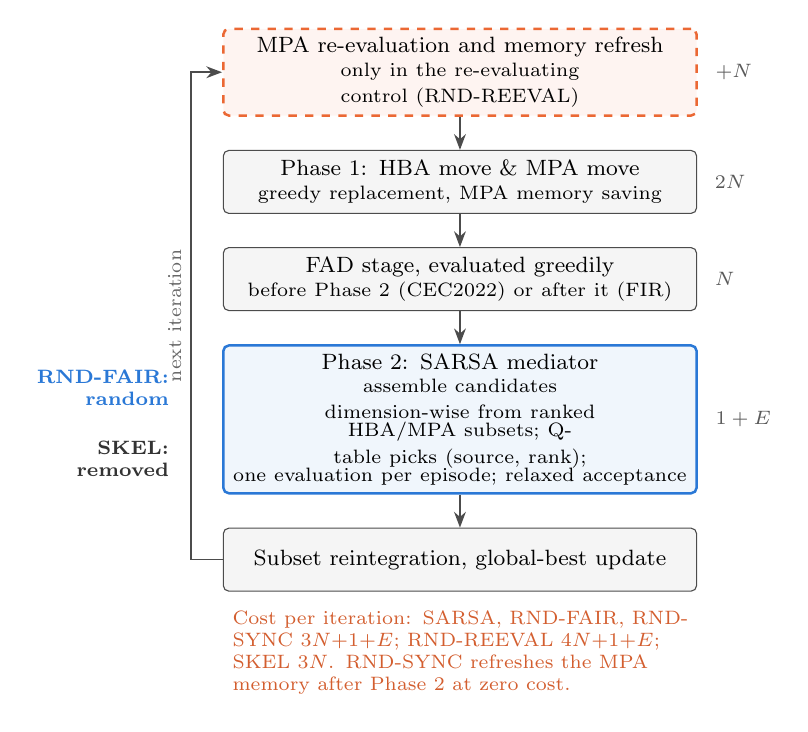
\begin{tikzpicture}[
  font=\footnotesize,
  node distance=4.2mm,
  box/.style={draw=black!70, rounded corners=2pt, fill=black!4, align=center,
              text width=58mm, inner sep=3pt, minimum height=8mm},
  med/.style={box, draw=lblue, line width=0.9pt, fill=lblue!7},
  extra/.style={box, draw=lorange, dashed, line width=0.9pt, fill=lorange!7},
  cost/.style={font=\scriptsize\itshape, text=black!65, anchor=west, align=left},
  tag/.style={font=\scriptsize\bfseries, text=black!80, anchor=east, align=right},
  arr/.style={-{Stealth[length=2mm]}, black!70, line width=0.6pt}]
  \node[extra] (re) {MPA re-evaluation and memory refresh\\[-1pt]
        {\scriptsize only in the re-evaluating control (RND-REEVAL)}};
  \node[box, below=of re] (p1) {Phase 1: HBA move \& MPA move\\[-1pt]{\scriptsize greedy replacement, MPA memory saving}};
  \node[box, below=of p1] (fad) {FAD stage, evaluated greedily\\[-1pt]
        {\scriptsize before Phase 2 (CEC2022) or after it (FIR)}};
  \node[med, below=of fad] (p2) {Phase 2: SARSA mediator\\[-1pt]
        {\scriptsize assemble candidates dimension-wise from ranked}\\[-3pt]
        {\scriptsize HBA/MPA subsets; Q-table picks (source, rank);}\\[-3pt]
        {\scriptsize one evaluation per episode; relaxed acceptance}};
  \node[box, below=of p2] (ri) {Subset reintegration, global-best update};

  \node[cost] at ($(re.east)+(1mm,0)$) {$+N$};
  \node[cost] at ($(p1.east)+(1mm,0)$) {$2N$};
  \node[cost] at ($(fad.east)+(1mm,0)$) {$N$};
  \node[cost] at ($(p2.east)+(1mm,0)$) {$1+E$};

  \draw[arr] (re) -- (p1);
  \draw[arr] (p1) -- (fad);
  \draw[arr] (fad) -- (p2);
  \draw[arr] (p2) -- (ri);
  \draw[arr] (ri.west) -- ++(-4mm,0) |- node[pos=0.25, rotate=90, above, font=\scriptsize, text=black!60]
        {next iteration} (re.west);

  \node[tag, text=lblue] at ($(p2.west)+(-5.5mm,4mm)$) {RND-FAIR:\\random};
  \node[tag] at ($(p2.west)+(-5.5mm,-5mm)$) {SKEL:\\removed};
  \node[font=\scriptsize, text=lorange!90!black, align=left, anchor=north west, text width=58mm]
        at ($(ri.south west)+(0,-1.2mm)$)
        {Cost per iteration: SARSA, RND-FAIR, RND-SYNC $3N{+}1{+}E$; RND-REEVAL $4N{+}1{+}E$; SKEL $3N$.
         RND-SYNC refreshes the MPA memory after Phase 2 at zero cost.};
\end{tikzpicture}
}
\caption{One iteration of the hybrid with its evaluation cost ($N$ agents per population, $E$ mediator episodes). The dashed
block exists only in the re-evaluating control. The arms of Study~I replace the mediator's policy (RND-FAIR), remove
Phase~2 (SKEL), or refresh the memory after Phase~2 at no cost (RND-SYNC).}
\label{fig:loop}
\end{figure}

%% =====================================================================
\section{What a control measures}
\label{sec:control}

\paragraph{Definition} Let $\mathcal A$ be an algorithm whose decisions in a component $\mathcal C$ are taken by a learned
policy, and $\mathcal A_0$ the same algorithm with $\mathcal C$'s decisions drawn from a reference distribution.
$\mathcal A_0$ is \emph{budget-matched} if both variants spend the same number of FEs in every iteration, so that they run
the same number of iterations under the same budget, and \emph{state-matched} if, given the same decisions, both perform
the same updates of every state variable outside the learned component (populations, memories, archives, parameters).

Write $Y(\pi,T,U)$ for the final error of a run that takes the component's decisions with policy $\pi$, runs $T$ iterations
and updates its state with rule $U$, and let a control use the reference policy $\pi_0$, $T_0$ iterations and rule $U_0$.

\begin{proposition}[What a control measures]
\label{prop:identify}
The contrast between the learned variant and a control decomposes exactly as
\begin{equation}
\begin{aligned}
\E Y(\pi,T,U)-\E Y(\pi_0,T_0,U_0)
&=\underbrace{\E Y(\pi,T,U)-\E Y(\pi_0,T,U)}_{\text{learning}}
+\underbrace{\E Y(\pi_0,T,U)-\E Y(\pi_0,T_0,U)}_{\text{budget}}\\
&\quad+\underbrace{\E Y(\pi_0,T_0,U)-\E Y(\pi_0,T_0,U_0)}_{\text{state}} .
\end{aligned}
\label{eq:identify}
\end{equation}
The budget term vanishes if $T_0=T$ and the state term if $U_0=U$; a budget- and state-matched control therefore measures
the learning term alone. For any other control the contrast is biased by the sum of the two other terms, whose sign is not
known in advance.
\end{proposition}
\begin{proof}
Add and subtract $\E Y(\pi_0,T,U)$ and $\E Y(\pi_0,T_0,U)$. For a budget-matched control, equal FEs per iteration give
$T_0=T$ (Proposition~\ref{prop:iter}); for a state-matched control $U_0=U$ by definition.
\end{proof}

The two other terms can be computed for a given hybrid. Runs stop at a total budget $B$ of FEs, and the number of iterations
is the largest that fits.

\begin{proposition}[Iterations under a fixed budget]
\label{prop:iter}
A variant that spends $a$ FEs on initialisation and $c$ FEs per iteration runs $T=\lfloor (B-a)/c\rfloor$ iterations.
MPHBS spends $c_\mathrm{S}=3N+1+E$ and a random control that re-evaluates the memory agents $c_\mathrm{R}=4N+1+E$, both with $a=2N$, because the
control evaluates the $N$ memory agents again at the start of each iteration. The control therefore runs
$T_\mathrm{R}/T_\mathrm{S}\approx(3N+1+E)/(4N+1+E)$ times as many iterations.
\end{proposition}
\begin{proof}
Every iteration of MPHBS evaluates the $N$ HBA proposals, the $N$ moved MPA agents, the $N$ FAD candidates, the start point
of the mediator and the $E$ episode candidates. The control executes the same steps and re-evaluates the $N$ MPA agents. The iteration count follows from the stopping rule.
\end{proof}

With $N=30$: on CEC2022 ($E=24$, $B=200{,}000$) $c_\mathrm{S}=115$ and $c_\mathrm{R}=145$, so $T_\mathrm{S}=1738$ and
$T_\mathrm{R}=1378$ ($-21\%$); on FIR ($E=72$, $B=150{,}000$) $c_\mathrm{S}=163$, $c_\mathrm{R}=193$, $T_\mathrm{S}=919$ and
$T_\mathrm{R}=776$ ($-16\%$).

\begin{proposition}[When the extra block matters]
\label{prop:memory}
With a deterministic objective, the control's start-of-iteration block (i) never changes a position and (ii) changes the
algorithm's state only through the memory update $(\tilde X^M,\tilde f^M)\gets(X^M,f^M)$. If the FAD stage follows Phase~2
(FIR), MPHBS performs the same update before the block, so the block has no effect other than its cost. If the FAD stage
precedes Phase~2 (CEC2022), MPHBS keeps the pre-Phase-2 memory, so the next memory saving compares moved MPA agents with
their pre-mediator positions, whereas the control compares them with the post-mediator population.
\end{proposition}
\begin{proof}
Between two evaluations of an MPA agent its position changes only by Phase~2, which writes back subset members that are
equal to or better than before. The re-evaluation therefore reproduces the stored values, $\tilde f^M_i<f^M_i$ never holds in
the block's memory saving, and no position reverts. The memory is last set by the FAD stage. If that stage follows Phase~2
the memory already equals the current population when the block runs; otherwise it predates Phase~2.
\end{proof}

The control also omits the value-table bookkeeping and a closest-action projection, which, once the table is not used, only
set table indices and draw no random numbers. We confirmed Proposition~\ref{prop:memory} and the inertness of these parts by
bit-identical re-runs (Section~\ref{sec:execution}). Algorithm~\ref{alg:protocol} turns the definition into a procedure.

\begin{algorithm}[!htbp]
\caption{Constructing and verifying a matched control for a learned component}
\label{alg:protocol}
\small
\begin{algorithmic}[1]
\Require implementation of $\mathcal A$ with learned component $\mathcal C$; reference distribution $q_0$
\Ensure control $\mathcal A_0$ and evidence that it is matched
\State implement $\mathcal A_0$ as a switch in the code path of $\mathcal A$ that replaces $\mathcal C$'s decisions by draws
  from $q_0$ and disables only the learning updates
\State \textbf{budget check:} measure FEs per iteration of $\mathcal A$ and $\mathcal A_0$; require equality and identical $T$
  under every budget used
\State \textbf{state check:} with $q_0$ set to the decisions of $\mathcal A$ (replay), require bit-identical trajectories of
  $\mathcal A$ and $\mathcal A_0$ for fixed seeds
\State \textbf{inertness checks:} for every difference not intended to matter, require bit-identical trajectories with and
  without it
\State \textbf{no-component arm:} add a variant without $\mathcal C$ to separate the value of the mechanism from that of learning
\State fix hypotheses, run counts and decision rule before running; report magnitudes alongside consistency measures
\end{algorithmic}
\end{algorithm}

%% =====================================================================
\section{What the value table can learn}
\label{sec:theory}

Section~\ref{sec:control} concerns the control. This section asks what the learned component itself can achieve, and
derives two properties of the value table from the update rule~\eqref{eq:sarsa}. Write $\sigma_d=(n_d,c_d)$ for the
provenance of coordinate $d$ of the current vector $v$ (the rank and source it was copied from) and $a_d=(n'_d,c'_d)$ for
the provenance chosen for the evaluated candidate $v'$. In the terms of SARSA, $\sigma$ is the state and $a$ the action, but
both index the same table.

\begin{proposition}[Credit assignment]
\label{prop:credit}
In episode $e$, the update~\eqref{eq:sarsa} changes only the entries $Q_{d,\sigma_d}$, $d\in A_e$. Consequently (i) the
choices $a_d$ of a rejected candidate receive no update, and (ii) an entry $Q_{d,n,c}$ is updated only in episodes in which
coordinate $d$ of the current vector was copied from rank $n$ of source $c$, with the reward of a candidate whose coordinate
$d$ was, in general, chosen differently.
\end{proposition}
\begin{proof}
The update writes $Q_{d,\sigma_d}\gets Q_{d,\sigma_d}+\alpha(r_e+\gamma Q_{d,a_d}-Q_{d,\sigma_d})$ if $v'$ is accepted and
$Q_{d,\sigma_d}\gets Q_{d,\sigma_d}+\alpha(r_e+\gamma Q_{d,\sigma_d}-Q_{d,\sigma_d})$ otherwise (as implemented in the
reference code and in our port). No other entry is written. Only an accepted candidate becomes the
current vector, so $\sigma_d$ changes to $a_d$ only after acceptance.
\end{proof}

The table therefore does not estimate how good it is to \emph{choose} a provenance, which is how the greedy policies use
it, but how often a search step \emph{from} a vector with that provenance fails. With acceptance rates of a few percent,
almost all updates are of the second kind. The next result bounds how precisely even that quantity can be estimated.

\begin{proposition}[Noise floor of a table entry]
\label{prop:noise}
Consider one entry and the sequence of its updates with rejected candidates. If the rewards of these updates are independent
with mean $\mu$ and variance $s^2$, the entry follows $Q_k=(1-\beta)Q_{k-1}+\alpha r_k$ with $\beta=\alpha(1-\gamma)$, and
\begin{equation}
\lim_{k\to\infty}\E[Q_k]=\frac{\mu}{1-\gamma},\qquad
\lim_{k\to\infty}\mathrm{Var}[Q_k]=\frac{\alpha^2 s^2}{\beta(2-\beta)}.
\label{eq:noise}
\end{equation}
The entry is an exponentially weighted average with an effective memory of $1/\beta$ updates.
\end{proposition}
\begin{proof}
For a rejected candidate the target is $r_k+\gamma Q_{k-1}$, so $Q_k=Q_{k-1}+\alpha(r_k+\gamma Q_{k-1}-Q_{k-1})
=(1-\beta)Q_{k-1}+\alpha r_k$. Unrolling, $Q_k=(1-\beta)^kQ_0+\alpha\sum_{j=0}^{k-1}(1-\beta)^j r_{k-j}$; the mean converges to
$\alpha\mu/\beta=\mu/(1-\gamma)$ and, by independence, the variance to
$\alpha^2 s^2\sum_j(1-\beta)^{2j}=\alpha^2s^2/(1-(1-\beta)^2)$.
\end{proof}

With $\alpha=0.1$ and $\gamma=0.3$, $\beta=\res{A-th-beta}$: an entry averages over about \res{A-th-memory} updates, and its
noise standard deviation is $\res{A-th-sdfactor}\,s$, independent of the length of the run.

\begin{corollary}[Ordering two choices]
\label{cor:order}
Let two entries satisfy Proposition~\ref{prop:noise} with mean rewards differing by $\Delta$, a common variance $s^2$ and
independent noise. In the stationary regime and under a normal approximation, the entry with the higher mean reward also has
the higher value with probability $\Phi(z)$, where
\begin{equation}
z=\frac{\Delta/(1-\gamma)}{\sqrt{2}\,\alpha s/\sqrt{\beta(2-\beta)}} .
\label{eq:order}
\end{equation}
\end{corollary}

A greedy choice is informative only if $z$ is well above 1, i.e.\ if the true differences between choices are large relative
to the reward noise and persist for many more than $1/\beta$ updates. Neither condition is a property of SARSA in general;
both follow from the parameters and the reward structure of this mediator, and both can be measured
(Section~\ref{sec:theorycheck}).

\paragraph{Consequence for a changing frame} The table is indexed by coordinates. If the mediator works in a frame that
changes from one iteration to the next (Section~\ref{sec:eigen}), the meaning of an entry changes with it, and what an entry
has averaged over the last $1/\beta$ updates no longer refers to one set of directions. This is an additional reason, besides
the evidence of Section~\ref{sec:results}, to pair the eigen-frame exchange with the uniform policy.

%% =====================================================================
\section{A rotation-invariant exchange}
\label{sec:eigen}

\subsection{Why the exchange depends on the coordinate system}
Consider a separable objective $f(x)=\sum_d g_d(x_d)$. If two good solutions $a$ and $b$ are good in different coordinates,
the candidate that takes the good coordinates of each is better than both: coordinate-wise exchange combines building
blocks. Now rotate the problem, $f_Q(x)=f(xQ^\top)$ with an orthogonal $Q$. The building blocks are now the projections onto
the columns of $Q$, and copying raw coordinates mixes them. For an ill-conditioned rotated function such as the ellipsoid,
even two nearby good solutions can produce, by coordinate-wise exchange, a candidate that leaves the narrow valley in which
both lie. Such candidates are rejected, the exchange stalls, and the hybrid loses the channel through which its populations
cooperate. The populations themselves carry the information needed to correct this: late in the search their members are
spread along the valley they occupy, so the principal axes of their covariance approximate the directions in which the
objective varies slowly or quickly.

\subsection{The eigen-frame exchange}
At the start of Phase~2, with probability $q$, the mediator computes the sample covariance of the pooled populations and its
eigendecomposition,
\begin{equation}
C = \mathrm{cov}\!\begin{pmatrix} X^H \\ X^M \end{pmatrix} = B\Lambda B^\top,
\label{eq:cov}
\end{equation}
with an orthonormal eigenvector matrix $B$ whose columns are ordered by eigenvalue. All operations of the mediator in this
iteration are then performed on the eigen coordinates $z=xB$ (Algorithm~\ref{alg:mediator}, lines~\ref{line:frame}--\ref{line:policy}):
the tensor $R$ holds the projected subsets, candidates are assembled coordinate-wise in $z$, the proxy
score~\eqref{eq:proxy} is computed on eigen coordinates, the selected candidate is mapped back and clipped,
$x'=\mathrm{clip}(z'B^\top)$, and, if accepted, its eigen coordinates are recomputed from the clipped point so that the
current vector always corresponds to a feasible evaluated point. With probability $1-q$ the iteration uses the original axes
($B=I$) and is identical to the random-mediator hybrid. We call the hybrid with $q=0.5$ and the uniform policy
\emph{EIG-MPHBS}. Fig.~\ref{fig:architecture} shows the architecture.

\begin{figure}[!htbp]
\centering
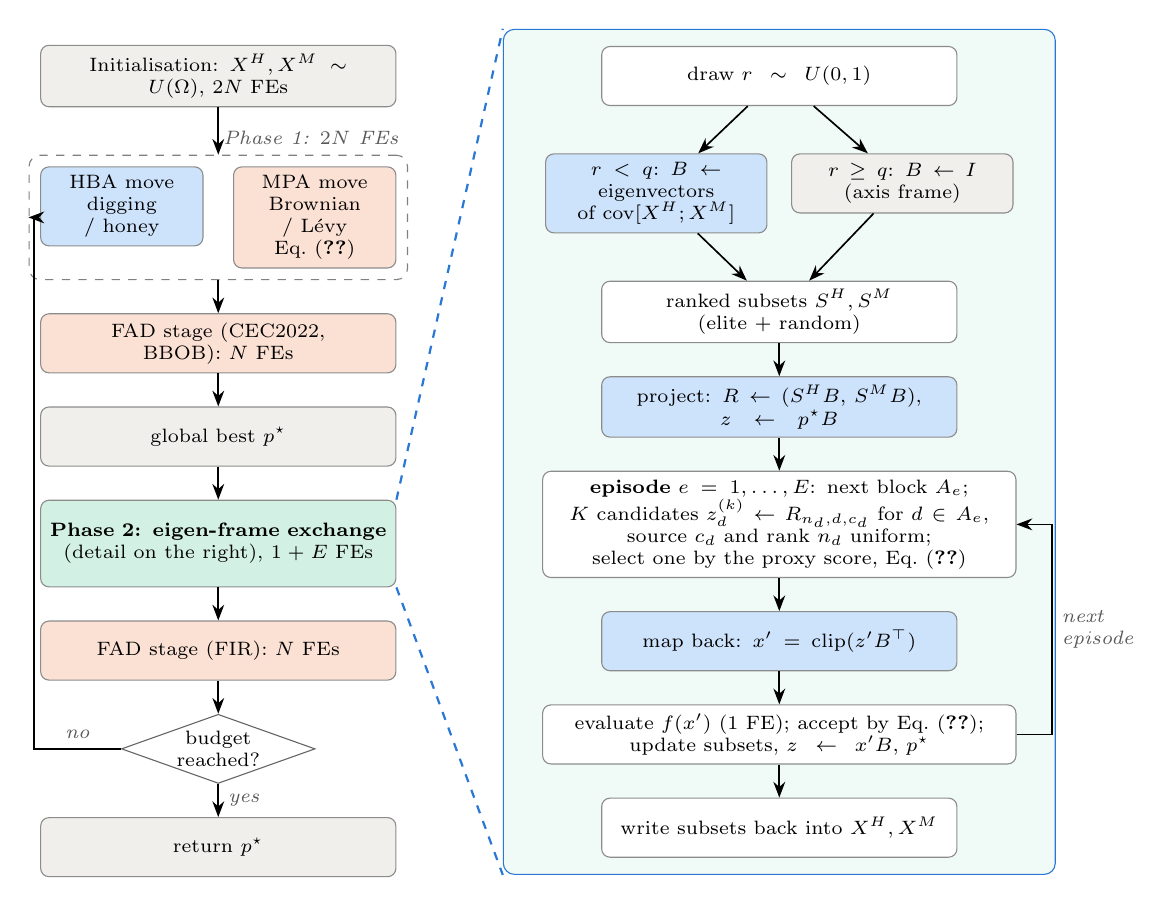
\begin{tikzpicture}[
  font=\scriptsize,
  node distance=0.42cm,
  blk/.style={draw=black!45, fill=#1, rounded corners=3pt, align=center, minimum height=0.75cm,
              text width=4.3cm, inner sep=3pt},
  dec/.style={draw=black!60, fill=white, diamond, aspect=2.8, align=center, inner sep=0.5pt},
  arr/.style={-{Stealth[length=2mm]}, semithick},
  lbl/.style={font=\scriptsize\itshape, text=black!65}]
% ---------------- left: one iteration
\node[blk=cgray] (init) {Initialisation: $X^H, X^M \sim U(\Omega)$, $2N$ FEs};
\node[blk=cblueL, text width=1.85cm, below=0.75cm of init.south west, anchor=north west] (hba) {HBA move\\digging / honey};
\node[blk=corangeL, text width=1.85cm, below=0.75cm of init.south east, anchor=north east] (mpa) {MPA move\\Brownian / L\'evy\\Eq.~\eqref{eq:memory}};
\node[draw=black!50, dashed, rounded corners, fit=(hba)(mpa), inner sep=4pt] (ph1) {};
\node[lbl, anchor=south east] at (ph1.north east) {Phase 1: $2N$ FEs};
\node[blk=corangeL, below=of ph1] (fad1) {FAD stage (CEC2022, BBOB): $N$ FEs};
\node[blk=cgray, below=of fad1] (gb) {global best $p^\star$};
\node[blk=cgreenL, below=of gb, minimum height=1.1cm] (p2) {\textbf{Phase 2: eigen-frame exchange}\\(detail on the right), $1+E$ FEs};
\node[blk=corangeL, below=of p2] (fad2) {FAD stage (FIR): $N$ FEs};
\node[dec, below=of fad2] (stop) {budget\\reached?};
\node[blk=cgray, below=of stop] (out) {return $p^\star$};
\draw[arr] (init) -- (ph1);
\draw[arr] (ph1) -- (fad1);
\draw[arr] (fad1) -- (gb);
\draw[arr] (gb) -- (p2);
\draw[arr] (p2) -- (fad2);
\draw[arr] (fad2) -- (stop);
\draw[arr] (stop) -- node[lbl, right] {yes} (out);
\draw[arr] (stop.west) -- node[lbl, above] {no} ++(-1.1,0) |- (ph1.west);
% ---------------- right: Phase 2 detail
\node[blk=white, right=2.6cm of init] (gate) {draw $r\sim U(0,1)$};
\node[blk=cblueL, text width=2.6cm, below=0.6cm of gate.south, anchor=north east, xshift=-0.15cm] (eig) {$r<q$: $B\gets$ eigenvectors\\of $\mathrm{cov}[X^H;X^M]$};
\node[blk=cgray, text width=2.6cm, below=0.6cm of gate.south, anchor=north west, xshift=0.15cm] (axis) {$r\ge q$: $B\gets I$\\(axis frame)};
\node[blk=white, below=0.6cm of gate |- eig.south] (sub) {ranked subsets $S^H, S^M$ (elite + random)};
\node[blk=cblueL, below=of sub] (proj) {project: $R\gets(S^HB,\,S^MB)$,\\$z\gets p^\star B$};
\node[blk=white, text width=5.8cm, below=of proj] (ep) {\textbf{episode} $e=1,\dots,E$: next block $A_e$;\\
  $K$ candidates $z^{(k)}_d\gets R_{n_d,d,c_d}$ for $d\in A_e$,\\
  source $c_d$ and rank $n_d$ uniform;\\
  select one by the proxy score, Eq.~\eqref{eq:proxy}};
\node[blk=cblueL, below=of ep] (back) {map back: $x'=\mathrm{clip}(z'B^\top)$};
\node[blk=white, text width=5.8cm, below=of back] (acc) {evaluate $f(x')$ (1 FE); accept by Eq.~\eqref{eq:accept};\\
  update subsets, $z\gets x'B$, $p^\star$};
\node[blk=white, below=of acc] (wb) {write subsets back into $X^H, X^M$};
\draw[arr] (gate) -- (eig);
\draw[arr] (gate) -- (axis);
\draw[arr] (eig) -- (sub);
\draw[arr] (axis) -- (sub);
\draw[arr] (sub) -- (proj);
\draw[arr] (proj) -- (ep);
\draw[arr] (ep) -- (back);
\draw[arr] (back) -- (acc);
\draw[arr] (acc.east) -- ++(0.45,0) |- node[lbl, right, pos=0.25, align=left] {next\\episode} (ep.east);
\draw[arr] (acc) -- (wb);
\begin{scope}[on background layer]
\node[draw=cblue, fill=cgreenL!35, rounded corners, fit=(gate)(eig)(axis)(ep)(wb), inner xsep=14pt, inner ysep=6pt] (detail) {};
\end{scope}
\draw[dashed, cblue, thick] (p2.north east) -- (detail.north west);
\draw[dashed, cblue, thick] (p2.south east) -- (detail.south west);
\end{tikzpicture}

\caption{Architecture of the eigen-frame hybrid. Left: one iteration. Right: the eigen-frame exchange (Phase~2). Blue boxes
are the only additions to the random-mediator hybrid; they use no function evaluations.}
\label{fig:architecture}
\end{figure}

\paragraph{Design choices} The exchange uses the uniform policy: the learner brings no measurable benefit at the same budget
(Study~I), and its table is indexed by coordinates whose meaning would change with the frame (Section~\ref{sec:theory}). The
frame probability is $q=0.5$: the axis frame remains useful on separable structure, where coordinate-wise exchange combines
building blocks, and mixing the two keeps both kinds of exchange. The value $q=0.5$ was chosen over $q=1$ in a 10-run pilot
on 32 instances (BBOB f1, f3, f8, f10, f12, f15, f16, f21; CEC2022 $D=20$; FIR), reported in Section~\ref{sec:ablation};
these instances are excluded from the confirmatory test of Study~II. Rotation can move a recombined point outside the box;
we clip after mapping back, which leaves the evaluation budget unchanged.

\subsection{Properties}
\begin{proposition}[Rotation invariance of the exchange]
\label{prop:invariance}
Let $Q$ be an orthogonal matrix and $\tilde f(y)=f(yQ^\top)$. Suppose the populations, subsets and global best of the rotated
run are the rotated images $\tilde X=XQ$ of those of the original run, the pooled covariance has distinct eigenvalues, the
same random numbers are drawn, and no clipping occurs. Then the eigen-frame exchange produces, in every episode, the
candidate $\tilde x'=x'Q$, with the same objective value and the same acceptance decision.
\end{proposition}
\begin{proof}
The pooled covariance of the rotated populations is $\tilde C=Q^\top CQ$, which has the same eigenvalues as $C$ and, since
they are distinct, eigenvectors $\tilde B=Q^\top BS$ with $S$ a diagonal matrix of signs, in the same order. The eigen
coordinates of a rotated point are therefore $\tilde z=xQ\,Q^\top BS=zS$: each coordinate equals the original one up to a
fixed sign. Ranks depend only on objective values, which are equal because $\tilde f(xQ)=f(x)$. Assembling a candidate by
copying coordinate $d$ from a stored solution commutes with multiplication by $S$, so $\tilde z'=z'S$. The terms of the proxy
score~\eqref{eq:proxy} are a mean rank, a mean of absolute coordinate differences and a Euclidean norm, all unchanged by
sign flips, so the same candidate is selected. Mapping back gives $\tilde x'=\tilde z'\tilde B^\top=z'SS^\top B^\top Q=x'Q$,
whose value is $\tilde f(x'Q)=f(x')$, and the acceptance rule depends only on objective values.
\end{proof}

\begin{remark}
The axis-frame exchange ($B=I$) has no such property. Proposition~\ref{prop:invariance} concerns the exchange step only:
the native moves of Phase~1 are coordinate-wise, and so is clipping, so the hybrid as a whole is not rotation invariant. A
unit test checks the invariance of the eigen coordinates numerically.
\end{remark}

\begin{proposition}[No extra evaluations]
\label{prop:cost}
In every iteration the eigen-frame hybrid performs exactly the same number of FEs as the random-mediator hybrid, $3N+1+E$.
The additional arithmetic is $O(ND^2+D^3)$ for the covariance and its eigendecomposition and $O(D^2)$ per episode for the
projections.
\end{proposition}
\begin{proof}
The frame is computed from points already evaluated, and the mediator evaluates one start point and one candidate per
episode in either frame. The covariance of $2N$ points costs $O(ND^2)$, the symmetric eigendecomposition $O(D^3)$, and each
projection of a $D$-vector $O(D^2)$.
\end{proof}

%% =====================================================================
\section{Design of the studies}
\label{sec:design}

The three studies share one framework: a Python implementation that counts every FE and in which all variants are switches
in one code path. Runs with the same benchmark, instance and run number share their seed across arms, so all comparisons are
seed-paired. Table~\ref{tab:studies} summarises the studies; they were designed and frozen one after the other, and
analyses added after a freeze are labelled post hoc or exploratory.

\begin{table}[!htbp]
\centering
\caption{The three studies. Pre-registered means that the hypotheses, run counts, statistics and decision rule were frozen
in a public repository before the runs; the confirmatory analysis script of Study~III was committed before its runs
finished.}
\label{tab:studies}
\footnotesize
\begin{tabular}{p{0.8cm}p{3.1cm}p{3.4cm}p{3.3cm}p{2.6cm}}
\toprule
Study & Question & Confirmatory hypotheses & Benchmarks, runs & Status \\
\midrule
I & Does learning matter? (Q1, Q2) & L1 learning; L2 published control; L3 mediator; L4 loop & CEC2022 $D=20$ (12), FIR (8); 50--100 runs per arm & pre-registered; BBOB extension and theory check exploratory \\
II & Does the eigen frame help? (Q3) & F1 vs random mediator; F2 vs learned hybrid (28 held-out instances) & CEC2022 $D=10,20$, BBOB $D=20$, FIR (56); 30 runs per algorithm & design document before confirmatory runs; held-out set \\
III & Does it transfer? (Q3) & T1 eigen vs axis for two parent pairs & BBOB $D=20$ (24), FIR (8); 30 runs per arm & pre-registered addendum; analysis script frozen \\
\bottomrule
\end{tabular}
\end{table}

\subsection{Benchmarks}
\begin{itemize}
\item CEC2022~\citep{kumar2021cec2022}, F1--F12 at $D=10$ and $D=20$, with the official code; budget $2\times10^5$ FEs.
\item BBOB~\citep{hansen2009bbob}, f1--f24 at $D=20$ (Study~I extension also $D=10$), with $10{,}000D$ or $2\times10^5$ FEs as
stated, and instance $((r-1)\bmod 15)+1$ in run $r$. It contains separable and rotated versions of the same functions, which
allows a direct test of rotation dependence.
\item Eight FIR filter-design problems ($D=31$) introduced with MPHBS~\citep{flores2026mphbs}: low-pass, high-pass,
band-pass and band-stop filters of order 30, each in an easier and a harder variant. The decision vector is the impulse
response $h\in[-1,1]^{31}$ and the objective is
\begin{equation}
F(h) = W_p\,\frac{1}{|P|}\sum_{n\in P}\bigl(|H(\omega_n)|-1\bigr)^2 + W_s\,\frac{1}{|S|}\sum_{n\in S}|H(\omega_n)|^2,
\label{eq:fir}
\end{equation}
where $H$ is the 2048-point discrete Fourier transform of $h$, $P$ and $S$ are the pass- and stop-band grid points, $W_p=1$
and $W_s\in\{100,120\}$. The budget is $1.5\times10^5$ FEs.
\end{itemize}
The outcome is the final error $f(x_\mathrm{best})-f^\star$ (the value $F$ on FIR, whose optimum is unknown), floored at
$10^{-8}$.

\subsection{Study I: arms and statistics}
\label{sec:armsI}
All arms use the configuration of the benchmark (Section~\ref{sec:hybrid}) and are listed in Table~\ref{tab:arms}.
\textbf{SARSA} is MPHBS unchanged. \textbf{RND-FAIR} draws $(c_d,n_d)$ uniformly and never reads or updates $Q$; everything
else, including the FE cost, is identical (budget- and state-matched). \textbf{RND-SYNC} (CEC2022 only) adds the control's
memory update at zero cost; by Proposition~\ref{prop:memory} it would equal RND-FAIR on FIR. \textbf{RND-AUTH} ports the
published control, including its extra evaluations. \textbf{SKEL} is the loop without Phase~2, and \textbf{MPHB} the
published backbone without mediator. The hypotheses are L1 (SARSA vs RND-FAIR: learning), L2a (RND-SYNC, or RND-FAIR on FIR,
vs RND-AUTH: budget of the control), L2b (RND-FAIR vs RND-SYNC on CEC2022: memory), L3 (SARSA vs SKEL: mediator) and L4
(SKEL vs MPHB: loop). L5--L8 (escape rate on F10, number of episodes, mediator components, memory update in SARSA) are
exploratory. The H1 pair was run 100 times per instance, every other arm 50 times.

% generated by scripts/paper_assets.py from configs/pathA.yaml -- do not edit
\begin{table*}[t]
\centering
\caption{Primary arms. All arms use the reference configuration of the domain (B-C1 on CEC2022, A-C1 on FIR)
and the same total budget (200{,}000 FE on CEC2022, 150{,}000 FE on FIR); the number of iterations $T$ follows from
the per-iteration cost. $N=30$; $E=24$ (CEC2022) and $72$ (FIR) mediator episodes per iteration.}
\label{tab:arms}
\small
\begin{tabular}{llcccc}
\toprule
 & & \multicolumn{2}{c}{FE per iteration} & \multicolumn{2}{c}{Iterations $T$} \\
\cmidrule(lr){3-4}\cmidrule(lr){5-6}
Arm & Change relative to MPHBS & CEC2022 & FIR & CEC2022 & FIR \\
\midrule
SARSA & none (reference: MPHBS) & 115 & 163 & 1738 & 919 \\
RND-FAIR & uniform random assembly, no Q-table & 115 & 163 & 1738 & 919 \\
RND-SYNC & RND-FAIR + zero-FE MPA memory refresh & 115 & -- & 1738 & -- \\
RND-REEVAL & random control with memory re-evaluation (+N FEs) & 145 & 193 & 1378 & 776 \\
SKEL & no Phase~2 (no mediator) & 90 & 90 & 2221 & 1666 \\
MPHB & backbone without mediator & 90 & 90 & 2221 & 1666 \\
\bottomrule
\end{tabular}
\end{table*}


For instance $j$ with $n$ seed pairs $(a_s,b_s)$ of anchor and comparator outcomes we compute the paired win probability
$\hat w_j=\frac1n\sum_s(\mathbb 1[a_s<b_s-\tau]+\frac12\mathbb 1[|a_s-b_s|\le\tau])$ with $\tau=10^{-12}$, the median relative
difference $\hat\delta_j=\mathrm{median}_s(b_s-a_s)/|b_s|$ (descriptive), and a two-sided Wilcoxon signed-rank
test~\citep{wilcoxon1945}, Holm-adjusted~\citep{holm1979} within each (hypothesis, benchmark) family. The domain-level effect
is $\bar W=\frac1J\sum_j\hat w_j$ with a 95\% percentile bootstrap interval~\citep{efron1979bootstrap}. The verdict is the
first that applies: \emph{mixed} if instances are Holm-significant in both directions; \emph{anchor superior} if some are in
favour of the anchor and the interval lies above 0.5; \emph{comparator superior} analogously; \emph{practically equivalent} if
none is significant and the interval lies in $[0.44,0.56]$, the negligible band of Vargha and Delaney~\citep{vargha2000};
otherwise \emph{inconclusive}.

\subsection{Study II: algorithms and statistics}
The hybrid family comprises EIG-MPHBS ($q=0.5$), MPHBS-R (the same code with the axis frame; this isolates the frame) and
MPHBS. HBA and MPA, ported from the reference code and validated against published per-run results, PSO, DE, GWO and WOA with
the standard settings of their publications, L-SHADE~\citep{tanabe2014lshade} and IPOP-CMA-ES~\citep{hansen2001cma,
auger2005ipop,hansen2019pycma} complete the eleven algorithms; all use the same budget. No algorithm is tuned beyond the
choice of $q$. Before any confirmatory run a design document fixed the algorithms, the benchmarks and two hypotheses on 28
held-out instances not used in any pilot (CEC2022 $D=10$ F1--F12; BBOB f2, f4--f7, f9, f11, f13, f14, f17--f20, f22--f24):
\textbf{F1} (EIG-MPHBS vs MPHBS-R, isolating the frame) and \textbf{F2} (vs MPHBS). For each instance the Vargha--Delaney
effect $A=P(e_1<e_2)+\frac12P(e_1=e_2)$ is computed over all $30\times30$ run pairs ($A>0.5$ favours the first algorithm), and
the median $A$ over instances is tested with a one-sided Wilcoxon signed-rank test of $A-0.5$, Holm over F1 and F2 at
$\alpha=0.05$. All other analyses of Study~II are secondary. The six classical algorithms were added after the main analysis
and are reported descriptively.

\subsection{Study III: transfer}
\label{sec:designIII}
The mediator and the eigen frame do not depend on HBA and MPA. In Study~III the two populations run the native moves of
another parent pair: PSO and DE (arms PD-R, PD-EIG) or GWO and WOA (GW-R, GW-EIG), with the axis frame (R) or the eigen
frame with $q=0.5$ (EIG). Everything else is common: the uniform policy, $N=30$, the mediator settings of the benchmark, no
FAD stage and no memory. \textbf{T1}: for each pair, the median $A$ of the eigen arm against its axis twin over the 32
instances (BBOB $D=20$ f1--f24 and FIR cases 1--8) exceeds 0.5, tested as in Study~II with Holm over the two pairs; per
instance $A$ uses all $30\times30$ run pairs. Seeds are paired with the other studies. The addendum was frozen before any of
its runs. Its scope was reduced, before any run, from three benchmarks to two because of compute (the CEC2022 instances were
dropped), and a timing test of 2 runs per arm on BBOB f2 and f10, recorded in the addendum, preceded the campaign. The
analysis script was committed before the campaign finished.

\subsection{Execution and validation}
\label{sec:execution}
Study~I ran once on GitHub-hosted Linux runners in a pinned environment after the full test suite had passed; Studies~II and
III ran on a 12-core laptop, one run per core, with every run seeded independently. The port's MPHBS reproduces the published
FE totals exactly and their published run distributions (the one known exception, a lower escape rate on CEC2022 F10, is
examined in Section~\ref{sec:resI}). Unit tests establish that (i) the variant code with default settings is bit-identical to
the validated MPHBS port; (ii) every arm's FE total matches Table~\ref{tab:arms}; (iii) at a fixed number of iterations the
published control produces trajectories bit-identical to RND-FAIR under the FIR configuration and to RND-SYNC under the
CEC2022 configuration, confirming Proposition~\ref{prop:memory}; (iv) removing the global-best copy does not change any
trajectory; (v) the eigen-frame and axis-frame hybrids use identical FE counts on every paired run, as
Proposition~\ref{prop:cost} states, and in Study~III on every instance of every pair. All runs of Study~I completed with the
expected FE totals; re-running its analysis on a second machine reproduced all verdicts, effect sizes and intervals.

%% =====================================================================
\section{Results}
\label{sec:results}

\subsection{Study I: learning, controls and the mediator}
\label{sec:resI}
Table~\ref{tab:primary} lists the confirmatory verdicts of Study~I and Fig.~\ref{fig:forest} all contrasts.

% generated by scripts/paper_assets.py -- do not edit
\begin{table*}[t]
\centering
\caption{Confirmatory contrasts (pre-registered L1--L4). Sig.\ (A/C): number of instances significant after Holm in favour of the anchor / comparator. $\bar W$: mean paired win probability of the anchor with 95\% bootstrap CI. Rel.\ diff.: median over instances of the median paired relative difference (comparator$-$anchor)/$|$comparator$|$ (positive: anchor lower; descriptive, not pre-registered). Verdicts by the frozen decision rule.}
\label{tab:primary}
\footnotesize
\setlength{\tabcolsep}{4pt}
\resizebox{\textwidth}{!}{%
\begin{tabular}{llllrccccl}
\toprule
 & Domain & Anchor & Comparator & $n$ & Sig.\ (A/C) & $\bar W$ & 95\% CI & Rel.\ diff. & Verdict \\
\midrule
L1 & CEC2022 & SARSA & RND-FAIR & 100 & 0/1 & 0.461 & [0.434, 0.489] & $-4.3{\times}10^{-4}$ & comparator \\
L1 & FIR & SARSA & RND-FAIR & 100 & 0/1 & 0.443 & [0.409, 0.476] & $-1.1{\times}10^{-2}$ & comparator \\
L2a & CEC2022 & RND-SYNC & RND-REEVAL & 50 & 0/0 & 0.534 & [0.495, 0.573] & $6.3{\times}10^{-12}$ & inconclusive \\
L2a & FIR & RND-FAIR & RND-REEVAL & 50 & 1/0 & 0.575 & [0.527, 0.623] & $1.4{\times}10^{-2}$ & anchor \\
L2b & CEC2022 & RND-FAIR & RND-SYNC & 50 & 9/2 & 0.717 & [0.690, 0.743] & $1.9{\times}10^{-1}$ & mixed \\
L3 & CEC2022 & SARSA & SKEL & 50 & 4/2 & 0.579 & [0.545, 0.613] & $1.0{\times}10^{-9}$ & mixed \\
L3 & FIR & SARSA & SKEL & 50 & 8/0 & 0.962 & [0.943, 0.980] & $5.4{\times}10^{-1}$ & anchor \\
L4 & CEC2022 & SKEL & MPHB & 50 & 12/0 & 0.780 & [0.757, 0.802] & $6.4{\times}10^{-11}$ & anchor \\
L4 & FIR & SKEL & MPHB & 50 & 8/0 & 0.826 & [0.798, 0.853] & $1.3{\times}10^{-8}$ & anchor \\
\bottomrule
\end{tabular}}
\end{table*}


\begin{figure}[!htbp]
\centering
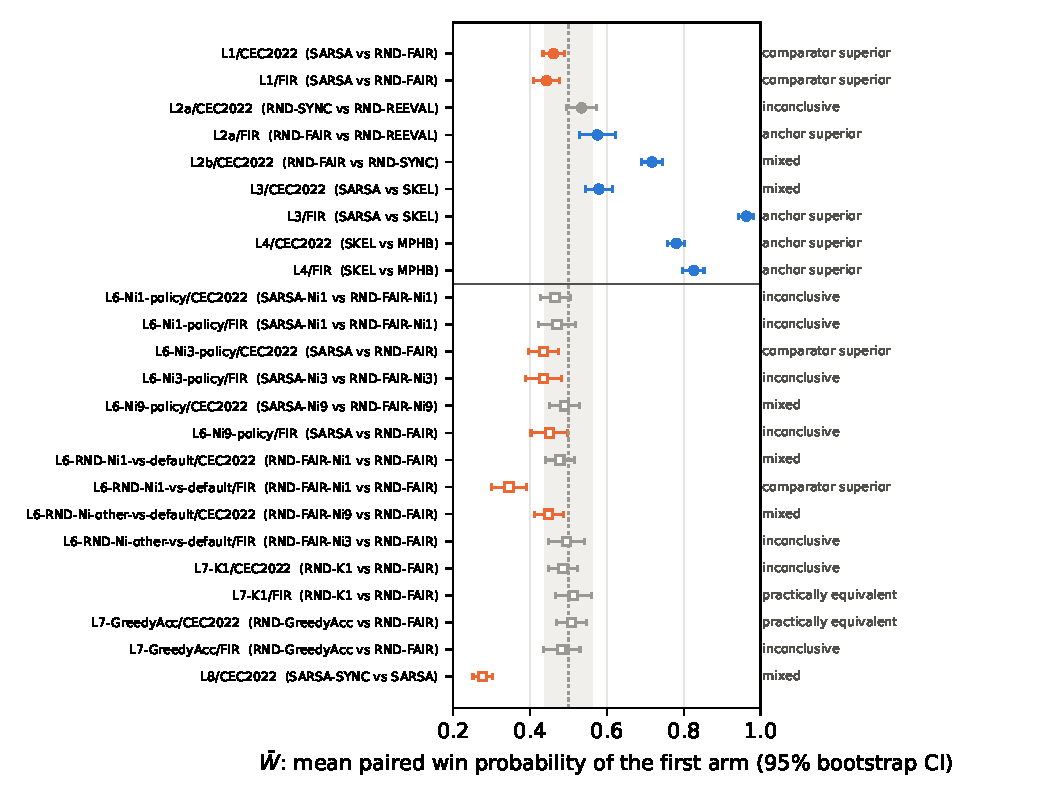
\includegraphics[width=0.78\textwidth]{figures/fig_forest.pdf}
\caption{Study I: mean paired win probability $\bar W$ of the first arm with 95\% bootstrap interval for every contrast
(circles: confirmatory; squares: exploratory; blue/orange: interval above/below 0.5). The shaded band is the
negligible-effect band of the decision rule.}
\label{fig:forest}
\end{figure}

\paragraph{Learning (L1)} At equal budget, SARSA does not outperform random assembly on either benchmark. On CEC2022 its mean
paired win probability is \res{A-H1-CEC2022-wbar} \res{A-H1-CEC2022-ci} and on FIR \res{A-H1-FIR-wbar} \res{A-H1-FIR-ci}. Both
intervals lie below 0.5, one instance per benchmark is significant in favour of the random mediator, and none favours SARSA,
so the pre-registered verdict is \emph{comparator superior} on both. The effect is small: the median relative difference is
$\res{A-H1-CEC2022-rel}$ on CEC2022 and $\res{A-H1-FIR-rel}$ on FIR (negative: SARSA's error is higher).

\paragraph{The re-evaluating control (L2)} With the memory update held fixed, the extra FEs of the control do not produce a
conclusive difference on CEC2022 ($\bar W=\res{A-H2a-CEC2022-wbar}$ \res{A-H2a-CEC2022-ci}, \emph{inconclusive}). On FIR,
where by Proposition~\ref{prop:memory} the extra block affects only the budget, the budget-identical random mediator is better
than the control ($\bar W=\res{A-H2a-FIR-wbar}$ \res{A-H2a-FIR-ci}, \emph{anchor superior}). The memory update has a large
effect on CEC2022 (L2b): random assembly \emph{without} the update beats the same mediator with it on \res{A-H2b-CEC2022-siga}
of 12 functions ($\bar W=\res{A-H2b-CEC2022-wbar}$ \res{A-H2b-CEC2022-ci}; median relative difference
$\res{A-H2b-CEC2022-rel}$), for instance on F5 with median errors of $\res{A-H2b-CEC2022-i5-amed}$ and
$\res{A-H2b-CEC2022-i5-cmed}$, while \res{A-H2b-CEC2022-sigc} functions favour the update; the verdict is \emph{mixed}. L2a and
L2b together explain the difference between the learned hybrid and a re-evaluating control without any contribution of
learning: it comes from the configuration of the control, mostly its memory update on CEC2022 and its reduced budget on FIR.
This is the budget and state term of Proposition~\ref{prop:identify}.

\paragraph{What matters (L3, L4)} Removing the mediator is very costly on FIR: SARSA beats SKEL on all eight cases
($\bar W=\res{A-H3-FIR-wbar}$ \res{A-H3-FIR-ci}; median relative difference $\res{A-H3-FIR-rel}$, i.e.\ the mediator roughly
halves the final objective). On CEC2022 the effect is mixed ($\bar W=\res{A-H3-CEC2022-wbar}$): the mediator helps markedly on
F1, F3, F9 and F10 and hurts on F5 and F7. Exchanging information between the populations is therefore useful, but its value
does not depend on learned choices. The restructured loop is consistently but negligibly better than the original backbone
(L4: $\bar W=\res{A-H4-CEC2022-wbar}$ and \res{A-H4-FIR-wbar}; median relative differences $\res{A-H4-CEC2022-rel}$ and
$\res{A-H4-FIR-rel}$): a paired design detects extremely consistent but tiny effects, and consistency measures must be
accompanied by magnitudes.

\paragraph{Exploratory results (L5--L8)} SARSA escapes the local basin of CEC2022 F10 in \res{A-H5-SARSA-esc}/\res{A-H5-SARSA-n}
runs (Wilson interval \res{A-H5-SARSA-ci}) and RND-FAIR in \res{A-H5-RND-FAIR-esc}/\res{A-H5-RND-FAIR-n}
(\res{A-H5-RND-FAIR-ci}; exact McNemar $p=\res{A-H5-mcnemar-p}$); the re-evaluating control escapes in
\res{A-H5-RND-AUTH-esc}/\res{A-H5-RND-AUTH-n} and SKEL in \res{A-H5-SKEL-esc}/\res{A-H5-SKEL-n}. Escaping requires the
mediator but not learning. Fewer episodes per iteration are clearly worse on FIR ($N_i=1$ against the default $9$: $\bar W=
\res{A-H6-RND-Ni1-vs-default-FIR-wbar}$ \res{A-H6-RND-Ni1-vs-default-FIR-ci}), while no tested $N_i$ shows a consistent
advantage of SARSA (Fig.~\ref{fig:dose}); removing proxy screening or relaxed acceptance leaves performance unchanged or
inconclusive; and adding the zero-cost memory update to SARSA reproduces the L2b pattern ($\bar W=\res{A-H8-CEC2022-wbar}$
\res{A-H8-CEC2022-ci}).

\begin{figure}[!htbp]
\centering
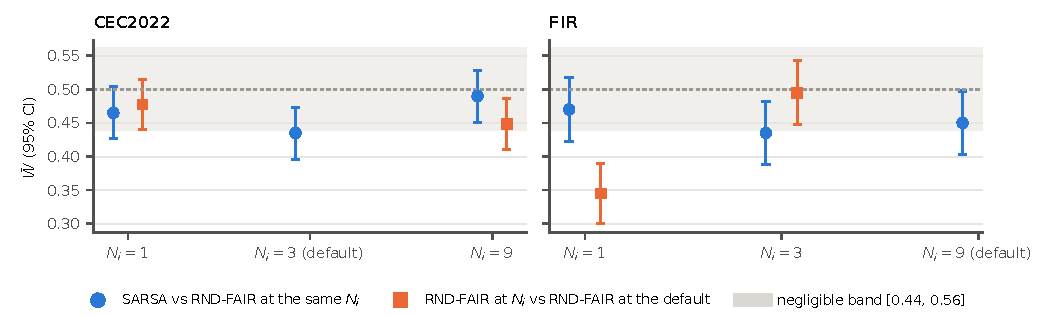
\includegraphics[width=0.85\textwidth]{figures/fig_dose.pdf}
\caption{Effect of the number of mediator episodes per subset member, $N_i$. Circles: SARSA vs RND-FAIR at the same $N_i$;
squares: RND-FAIR at $N_i$ vs RND-FAIR at the default $N_i$ of the benchmark.}
\label{fig:dose}
\end{figure}

\subsection{Study I: a check of the value-table properties}
\label{sec:theorycheck}
The propositions of Section~\ref{sec:theory} hold by construction; whether their consequences matter depends on the rewards
that the mediator produces. We logged every mediator episode of \res{A-th-runs} additional MPHBS runs (5 per instance, seeds
disjoint from the study): the reward, the provenance of the evaluated candidate's coordinates, and the table. For each cell
$(d,n,c)$ we computed the mean reward of the candidates whose coordinate $d$ was copied from rank $n$ of source $c$, which is
the quantity a useful table would have to rank (Table~\ref{tab:theory}). This check was not part of the pre-registration.

% generated by scripts/pathA_theory_assets.py -- do not edit
\begin{table*}[!t]
\centering
\caption{Post hoc check of Section~\ref{sec:theory} (5 runs per instance; medians over runs, interquartile ranges in
brackets). $p_+$: share of episodes with reward $+1$. $\sigma$: reward standard deviation. $\mathrm{sd}(Q)$: noise
standard deviation of a table entry predicted by Proposition~\ref{prop:noise}. $\hat\tau$: between-cell standard deviation
of the mean reward of the choices tried (method of moments, cells with at least 30 trials). $z$: separation of two
cells that differ by $\hat\tau$, Corollary~\ref{cor:order}. $\rho_{1/2}$: Spearman correlation of the cells' mean
rewards between the first and second half of the run. $\rho_Q$: Spearman correlation between the table at mid-run and
the cells' mean rewards in the second half.}
\label{tab:theory}
\footnotesize
\begin{tabular}{lcccccccc}
\toprule
Benchmark & runs & $p_+$ & $\sigma$ & $\mathrm{sd}(Q)$ & $\hat\tau$ & $z$ & $\rho_{1/2}$ & $\rho_Q$ \\
\midrule
CEC2022 ($D=20$) & 60 & 2.9\% & 0.35 & 0.094 & 0.045 & 0.58 & 0.57 [0.48, 0.66] & -0.39 [-0.46, -0.27] \\
FIR ($D=31$) & 40 & 12.5\% & 0.71 & 0.192 & 0.029 & 0.16 & 0.03 [0.00, 0.06] & 0.00 [-0.05, 0.04] \\
\bottomrule
\end{tabular}
\end{table*}


Rewards are sparse: \res{A-th-CEC-p_plus} of CEC2022 episodes and \res{A-th-FIR-p_plus} of FIR episodes improve on the current
vector, so almost every update is the rejected-candidate case of Propositions~\ref{prop:credit} and~\ref{prop:noise}. Between
cells, the mean reward of the choices tried differs by $\hat\tau=\res{A-th-CEC-tau_action}$ on CEC2022 and
$\res{A-th-FIR-tau_action}$ on FIR, which the noise floor turns into a separation of only $z=\res{A-th-CEC-z_typical}$ and
$\res{A-th-FIR-z_typical}$ (Corollary~\ref{cor:order}). The two benchmarks then differ. On FIR there is nothing stable to
learn: the cells' mean rewards in the two halves of a run are uncorrelated ($\rho_{1/2}=\res{A-th-FIR-split_half_rho}$), and so
is the table with later outcomes ($\rho_Q=\res{A-th-FIR-Qmid_validity_rho}$, positive in \res{A-th-FIR-valid-pos} of
\res{A-th-FIR-n} runs). On CEC2022 there is a stable signal ($\rho_{1/2}=\res{A-th-CEC-split_half_rho}$), but the table ranks
the cells against it: $\rho_Q=\res{A-th-CEC-Qmid_validity_rho}$, negative in all but \res{A-th-CEC-valid-pos} of
\res{A-th-CEC-n} runs. This is what Proposition~\ref{prop:credit} leads one to expect. A provenance that produces good vectors
keeps them current for many episodes, and in each of these episodes the table charges it with the failure of whatever
candidate is tried next; the better the provenance, the more penalties it collects. The noise floor would limit any table with
$\alpha=0.1$, while the credit assignment is specific to this mediator and would remain if $\alpha$ were changed.

\subsection{Study I: BBOB extension (exploratory)}
\label{sec:bbob}
To check whether L1 and L3 hold beyond the original two benchmark sets, SARSA, RND-FAIR and SKEL were run on the 24 BBOB
functions at $D=10$ and $D=20$ ($10{,}000D$ FEs, configuration B-C1, 30 paired runs per function; \res{A-bbob-runs} runs). At
$D=10$ SARSA and random assembly are practically equivalent ($\bar W=\res{A-bbob-B1-D10-wbar}$ \res{A-bbob-B1-D10-ci});
at $D=20$ the verdict is mixed (SARSA better on f3, random assembly on f9) and the interval for $\bar W$
(\res{A-bbob-B1-D20-wbar} \res{A-bbob-B1-D20-ci}) again lies below 0.5. The value of the mediator depends on the function
class (Table~\ref{tab:bbob-groups}): it helps strongly on separable or nearly separable functions and hurts on rotated,
ill-conditioned or non-separable ones such as f10, f12, f13 and f15, which matches its mechanism and motivates Study~II.

% generated by scripts/paper_bbob_assets.py -- do not edit
\begin{table*}[!t]
\centering
\caption{BBOB by function group: mean paired win probability of SARSA over the group's functions, and the number of
functions significant (Holm over all 24) in favour of SARSA / of the comparator.}
\label{tab:bbob-groups}
\footnotesize
\begin{tabular}{lcccc}
\toprule
 & \multicolumn{2}{c}{B1: SARSA vs RND-FAIR} & \multicolumn{2}{c}{B3: SARSA vs SKEL} \\
\cmidrule(lr){2-3}\cmidrule(lr){4-5}
Group & $D=10$ & $D=20$ & $D=10$ & $D=20$ \\
\midrule
separable (f1--f5) & 0.53 (0/0) & 0.54 (1/0) & 0.69 (2/0) & 0.70 (2/0) \\
low/moderate conditioning (f6--f9) & 0.45 (0/0) & 0.35 (0/1) & 0.50 (1/1) & 0.77 (2/0) \\
high conditioning (f10--f14) & 0.51 (0/0) & 0.40 (0/0) & 0.29 (0/2) & 0.49 (1/2) \\
multimodal, adequate structure (f15--f19) & 0.52 (0/0) & 0.41 (0/0) & 0.48 (0/2) & 0.46 (1/1) \\
multimodal, weak structure (f20--f24) & 0.49 (0/0) & 0.48 (0/0) & 0.40 (1/2) & 0.41 (1/3) \\
\bottomrule
\end{tabular}
\end{table*}


\subsection{Study II: the eigen-frame exchange}
\label{sec:resII}

\paragraph{Confirmatory tests (F1, F2)} On the 28 held-out instances, EIG-MPHBS is better than MPHBS-R on \res{E-H1-ngt}
instances, tied on \res{E-H1-neq} and worse on \res{E-H1-nlt} (one-sided $p=\res{E-H1-p}$), and better than MPHBS on
\res{E-H2-ngt}, tied on \res{E-H2-neq} and worse on \res{E-H2-nlt} ($p=\res{E-H2-p}$). After Holm correction both hypotheses
are supported ($p_\text{Holm}=\res{E-H1-pholm}$ for each; Table~\ref{tab:confirm}, Fig.~\ref{fig:heldout}). The evidence is
not strong: the median effects are small (\res{E-H1-medA} and \res{E-H2-medA}) because most CEC2022 $D=10$ functions are
solved equally well by all three variants, and when instances with $A=0.5$ are kept in the test with Pratt or zero-split
handling the Holm-adjusted $p$-values become \res{E-H1-pholm-pratt} and \res{E-H1-pholm-zsplit}. The rule fixed in advance
used the default handling; we report the alternatives so that readers can weigh the result. Per instance, EIG-MPHBS is
significantly better than MPHBS-R on \res{E-H1-sigfor} held-out instances (BBOB f6, f9, f11, f14, f19) and worse on
\res{E-H1-sigagainst} (f4, the separable Rastrigin variant); against MPHBS it is better on \res{E-H2-sigfor} and never
significantly worse. On all 56 instances the median $A$ is \res{E-S1-H1-medA} against MPHBS-R ($p=\res{E-S1-H1-p}$;
\res{E-S1-H1-sigfor} instances significantly better, \res{E-S1-H1-sigagainst} worse) and \res{E-S1-H2-medA} against MPHBS
($p=\res{E-S1-H2-p}$; \res{E-S1-H2-sigfor} better, \res{E-S1-H2-sigagainst} worse), with the largest effects on FIR (median
$A$ \res{E-S1-H2-FIR-medA}) and CEC2022 $D=20$ (\res{E-S1-H2-C20-medA}); these include the pilot instances on which $q$ was
chosen, so their effect sizes may be optimistic.

% generated by scripts/eswa_paper_assets.py -- do not edit
\begin{table}[!htbp]
\centering
\caption{Confirmatory tests on the 28 held-out instances (F1, F2) and their repetition on all 56 instances
(F1$'$, F2$'$, secondary: the 28 additional instances include those used to choose the eigen-frame probability).
$\tilde A$: median Vargha--Delaney effect over instances ($>0.5$ favours EIG-MPHBS). W/T/L: instances with
$A>0.5$, $A=0.5$, $A<0.5$. $p$: one-sided Wilcoxon signed-rank test of $A-0.5$ over instances; Holm over
\{F1, F2\}. The two sensitivity columns keep the instances with $A=0.5$ (Pratt and zero-split handling).
Sig.: instances where a paired per-instance test (Holm within benchmark) favours EIG-MPHBS / the comparator.}
\label{tab:confirm}
\footnotesize
\setlength{\tabcolsep}{4pt}
\resizebox{\textwidth}{!}{%
\begin{tabular}{llccccccc}
\toprule
 & Comparison & $\tilde A$ & W/T/L & $p$ & $p_\text{Holm}$ & $p_\text{Holm}$ (Pratt) & $p_\text{Holm}$ (zsplit) & Sig. \\
\midrule
F1 & EIG-MPHBS vs MPHBS-R & 0.500 & 14/6/8 & 0.031 & 0.043 & 0.056 & 0.057 & 5/1 \\
F2 & EIG-MPHBS vs MPHBS & 0.514 & 15/5/8 & 0.022 & 0.043 & 0.056 & 0.057 & 6/0 \\
\midrule
F1$'$ & all 56 instances (vs MPHBS-R) & 0.520 & 31/7/18 & \ensuremath{7.7{\times}10^{-4}} & -- & -- & -- & 12/1 \\
F2$'$ & all 56 instances (vs MPHBS) & 0.529 & 33/6/17 & \ensuremath{5.2{\times}10^{-4}} & -- & -- & -- & 14/0 \\
\bottomrule
\end{tabular}}
\end{table}


\begin{figure}[!htbp]
\centering
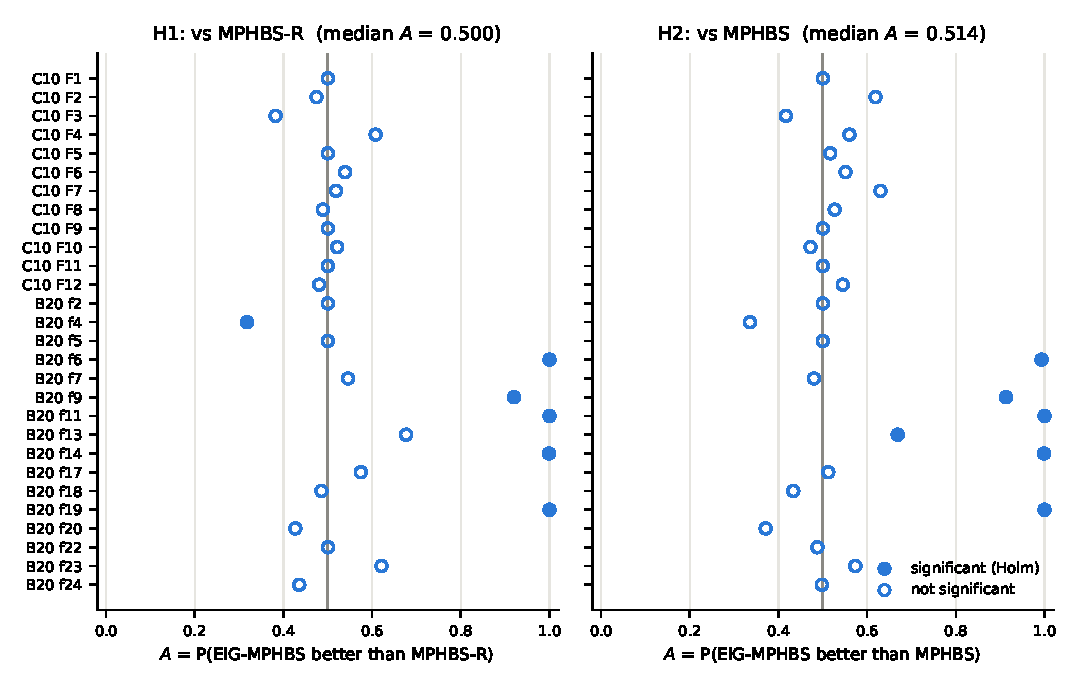
\includegraphics[width=\linewidth]{figures/fig_heldout.pdf}
\caption{Effect size $A$ of EIG-MPHBS on each of the 28 held-out instances against MPHBS-R (F1) and MPHBS (F2); $A>0.5$
favours EIG-MPHBS. Filled markers: significant per-instance paired test (Holm within benchmark). C10: CEC2022 $D=10$; B20:
BBOB $D=20$.}
\label{fig:heldout}
\end{figure}

\paragraph{Rotation dependence} Table~\ref{tab:rotation} compares BBOB functions that differ only by a rotation. On the
separable ellipsoid (f2) all algorithms reach the accuracy floor. On the rotated ellipsoid (f10), MPHBS and MPHBS-R stall at
median errors of \res{E-f10-MPHBS} and \res{E-f10-RND}, while EIG-MPHBS reaches \res{E-f10-EIG50}, a
\res{E-f10-ratio-RND}-fold reduction relative to MPHBS-R and \res{E-f10-ratio-MPHBS}-fold relative to MPHBS. On Rastrigin the
rotated version (f15) is hard for all three hybrids and the eigen frame does not help (median \res{E-f15-EIG50} against
\res{E-f15-RND} for MPHBS-R), and on the separable version (f3) EIG-MPHBS is slightly worse (\res{E-f3-EIG50} against
\res{E-f3-RND}), as expected when half of the exchanges no longer follow the axes along which the function separates. The gap
to CMA-ES and L-SHADE on f10 remains because Phase~1 is still coordinate-wise.

% generated by scripts/eswa_paper_assets.py -- do not edit
\begin{table}[!htbp]
\centering
\caption{Median final error on BBOB function pairs that differ only by a rotation ($D=20$, 30 runs; values at or
below $10^{-8}$ shown as 0).}
\label{tab:rotation}
\small
\begin{tabular}{lcccc}
\toprule
 & \multicolumn{2}{c}{Ellipsoid} & \multicolumn{2}{c}{Rastrigin} \\
\cmidrule(lr){2-3}\cmidrule(lr){4-5}
Algorithm & f2 (separable) & f10 (rotated) & f3 (separable) & f15 (rotated) \\
\midrule
EIG-MPHBS & 0 & 8.47 & 1.99 & 54.2 \\
MPHBS-R & 0 & 89.9 & 0.995 & 58.7 \\
MPHBS & 0 & 121 & 0.995 & 51.2 \\
CMA-ES & 0 & 0 & 8.95 & 2.98 \\
L-SHADE & 0 & 0 & 0 & 4.13 \\
\bottomrule
\end{tabular}
\end{table}


\paragraph{Mechanism} Fig.~\ref{fig:mechanism} shows the fraction of exchanged candidates that are accepted in each iteration
and the diversity of the populations. On the rotated ellipsoid f10 the axis-frame exchange almost stops working after the first
few thousand evaluations: in the first quarter of the budget \res{E-acc-B20-10-RND}\% of the candidates of MPHBS-R and
\res{E-acc-B20-10-MPHBS}\% of those of MPHBS are accepted, against \res{E-acc-B20-10-EIG50}\% for EIG-MPHBS; the discus f11
shows the same pattern (\res{E-acc-B20-11-RND}\% and \res{E-acc-B20-11-MPHBS}\% against \res{E-acc-B20-11-EIG50}\%). Because
the candidates stay inside the valley, the populations contract faster along it. This supports the explanation of
Section~\ref{sec:eigen}: the frame restores the exchange channel on coupled problems rather than changing the native moves.

\begin{figure}[!htbp]
\centering
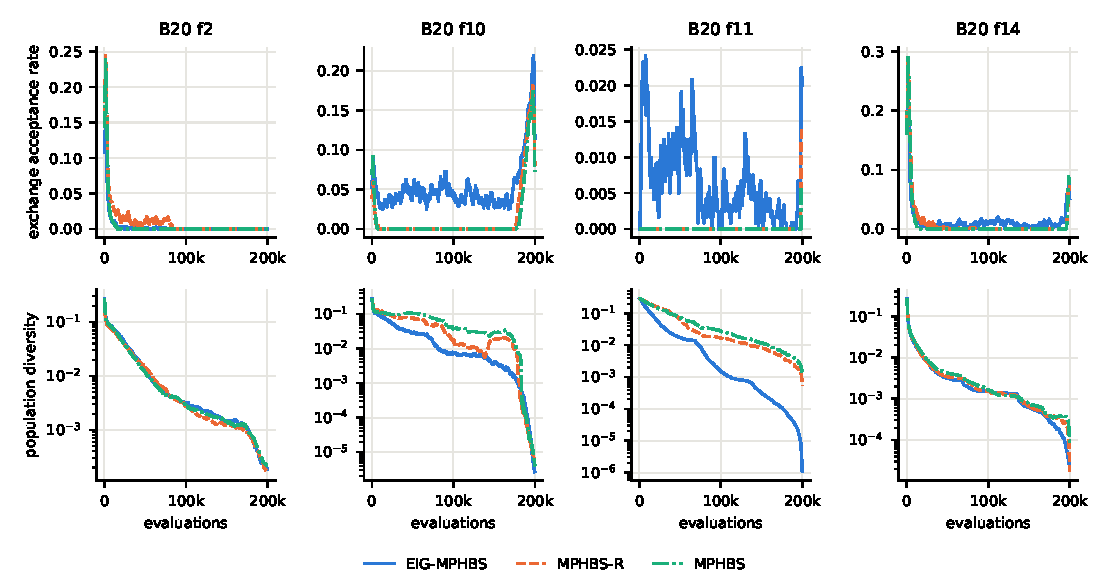
\includegraphics[width=\textwidth]{figures/fig_mechanism.pdf}
\caption{Mechanism of the eigen frame on BBOB $D=20$. Top: fraction of exchanged candidates accepted per iteration (moving
average over 25 iterations). Bottom: population diversity (log scale). Medians over 30 runs. f2 is separable; f10, f11 and f14
are rotated.}
\label{fig:mechanism}
\end{figure}

\paragraph{Comparison with ten algorithms} Fig.~\ref{fig:ranks} and Table~\ref{tab:ranks} give the mean Friedman
ranks~\citep{derrac2011tutorial} of the eleven algorithms and Table~\ref{tab:wtl} the per-instance significance of
EIG-MPHBS against each. EIG-MPHBS ranks \res{E-pos-EIG50} of 11 overall (mean rank \res{E-rank-EIG50}), behind L-SHADE
(\res{E-rank-L-SHADE}) and CMA-ES (\res{E-rank-CMA-ES}) and ahead of MPHBS-R (\res{E-rank-RND}), MPHBS (\res{E-rank-MPHBS}) and
all classical metaheuristics. It is significantly better than MPHBS on \res{E-win-MPHBS} instances and worse on none, better
than MPHBS-R on \res{E-win-RND} and worse on \res{E-loss-RND}, better than HBA on \res{E-win-HBA} of 56 and worse on none, and
better than MPA on \res{E-win-MPA} and worse on \res{E-loss-MPA}. Over PSO, DE, GWO and WOA it wins \res{E-common-win} and
loses \res{E-common-loss} of \res{E-common-n} comparisons; GWO and WOA are known to be biased towards the centre of the search
space~\citep{kudela2022centre}. L-SHADE and CMA-ES are clearly stronger at $D=20$, on BBOB and on FIR.

\begin{figure}[!htbp]
\centering
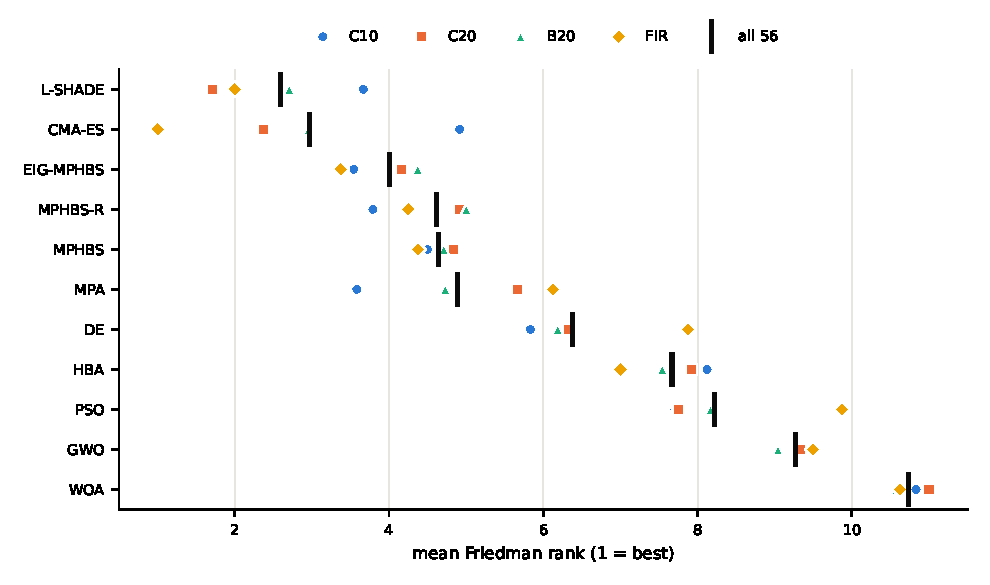
\includegraphics[width=0.92\linewidth]{figures/fig_ranks.pdf}
\caption{Mean Friedman rank of each algorithm per benchmark (markers) and over all 56 instances (vertical bar); 1 = best.
C10/C20: CEC2022 $D=10/20$; B20: BBOB $D=20$.}
\label{fig:ranks}
\end{figure}

% generated by scripts/eswa_paper_assets.py -- do not edit
\begin{table}[!htbp]
\centering
\caption{Mean Friedman rank of the eleven algorithms (rank of the median final error on each instance, 1 = best;
lowest in bold), per benchmark and over all 56 instances. Last row: Friedman test $p$ per benchmark.}
\label{tab:ranks}
\small
\begin{tabular}{lccccc}
\toprule
Algorithm & C10 & C20 & B20 & FIR & All \\
 & (12) & (12) & (24) & (8) & (56) \\
\midrule
L-SHADE & 3.67 & \textbf{1.71} & \textbf{2.71} & 2.00 & \textbf{2.60} \\
CMA-ES & 4.92 & 2.38 & 2.96 & \textbf{1.00} & 2.97 \\
EIG-MPHBS & \textbf{3.54} & 4.17 & 4.38 & 3.38 & 4.01 \\
MPHBS-R & 3.79 & 4.92 & 5.00 & 4.25 & 4.62 \\
MPHBS & 4.50 & 4.83 & 4.71 & 4.38 & 4.64 \\
MPA & 3.58 & 5.67 & 4.73 & 6.12 & 4.88 \\
DE & 5.83 & 6.33 & 6.19 & 7.88 & 6.38 \\
HBA & 8.12 & 7.92 & 7.54 & 7.00 & 7.67 \\
PSO & 7.71 & 7.75 & 8.17 & 9.88 & 8.22 \\
GWO & 9.50 & 9.33 & 9.04 & 9.50 & 9.27 \\
WOA & 10.83 & 11.00 & 10.58 & 10.62 & 10.73 \\
\midrule
Friedman $p$ & \ensuremath{3.9{\times}10^{-14}} & \ensuremath{1.3{\times}10^{-14}} & \ensuremath{2.8{\times}10^{-26}} & \ensuremath{1.4{\times}10^{-12}} & -- \\
\bottomrule
\end{tabular}
\end{table}

% generated by scripts/eswa_paper_assets.py -- do not edit
\begin{table}[!htbp]
\centering
\caption{EIG-MPHBS against each algorithm: number of instances where it is significantly better / not
significantly different / significantly worse (paired two-sided Wilcoxon signed-rank test over the 30 seed-paired
runs, Holm within each benchmark and comparator, $\alpha=0.05$).}
\label{tab:wtl}
\small
\begin{tabular}{lccccc}
\toprule
vs & C10 (12) & C20 (12) & B20 (24) & FIR (8) & Total (56) \\
\midrule
L-SHADE & 1/9/2 & 0/4/8 & 3/5/16 & 0/0/8 & 4/18/34 \\
CMA-ES & 3/7/2 & 1/5/6 & 4/5/15 & 0/0/8 & 8/17/31 \\
MPHBS-R & 0/12/0 & 3/9/0 & 7/16/1 & 2/6/0 & 12/43/1 \\
MPHBS & 0/12/0 & 2/10/0 & 7/17/0 & 5/3/0 & 14/42/0 \\
MPA & 1/11/0 & 5/5/2 & 10/10/4 & 8/0/0 & 24/26/6 \\
DE & 9/2/1 & 7/3/2 & 13/8/3 & 8/0/0 & 37/13/6 \\
HBA & 10/2/0 & 10/2/0 & 19/5/0 & 8/0/0 & 47/9/0 \\
PSO & 9/3/0 & 9/3/0 & 18/5/1 & 8/0/0 & 44/11/1 \\
GWO & 12/0/0 & 12/0/0 & 20/4/0 & 8/0/0 & 52/4/0 \\
WOA & 12/0/0 & 12/0/0 & 24/0/0 & 8/0/0 & 56/0/0 \\
\bottomrule
\end{tabular}
\end{table}


\paragraph{Comparison with EA4eig and cost} EA4eig~\citep{bujok2022ea4eig}, which combines eigen crossover with four strong
algorithms, is significantly better than EIG-MPHBS on \res{E-ea4eig-D10-worse} of 12 CEC2022 functions at $D=10$ and
\res{E-ea4eig-D20-worse} of 12 at $D=20$ at the competition budgets (official results; unpaired, descriptive;
Table~\ref{tab:ea4eig}), and EIG-MPHBS is never significantly better. The eigen frame adds
\res{E-overhead-min}--\res{E-overhead-max}\% to the median run time of MPHBS-R, and EIG-MPHBS is faster than MPHBS, whose
SARSA bookkeeping costs more than the decomposition (Table~\ref{tab:cost}).

% generated by scripts/eswa_paper_assets.py -- do not edit
\begin{table}[!htbp]
\centering
\caption{EIG-MPHBS against the official CEC2022 runs of EA4eig at the competition budgets ($2\times10^5$
evaluations for $D=10$, $10^6$ for $D=20$; 30 runs each). Median final error (at or below $10^{-8}$ shown as 0) and
Vargha--Delaney $A$ ($>0.5$ favours EIG-MPHBS). Superscripts: two-sided Mann--Whitney test, Holm over the 12
functions of each dimension ($^{+}$ EIG-MPHBS better, $^{-}$ worse, $^{\approx}$ no significant difference).
Unpaired and descriptive: hardware and implementation differ.}
\label{tab:ea4eig}
\small
\begin{tabular}{lcccccc}
\toprule
 & \multicolumn{3}{c}{$D=10$} & \multicolumn{3}{c}{$D=20$} \\
\cmidrule(lr){2-4}\cmidrule(lr){5-7}
 & EIG-MPHBS & EA4eig & $A$ & EIG-MPHBS & EA4eig & $A$ \\
\midrule
F1 & 0$^{\approx}$ & 0 & 0.50 & 0$^{\approx}$ & 0 & 0.50 \\
F2 & 0$^{\approx}$ & 0 & 0.46 & 47$^{-}$ & 0 & 0.17 \\
F3 & 2.27e-7$^{-}$ & 0 & 0.13 & 7.77e-8$^{-}$ & 0 & 0.15 \\
F4 & 7.96$^{-}$ & 0.995 & 0.01 & 34.8$^{-}$ & 6.96 & 0.00 \\
F5 & 0$^{\approx}$ & 0 & 0.50 & 14.1$^{-}$ & 0 & 0.00 \\
F6 & 0.155$^{-}$ & 5.41e-3 & 0.04 & 3.28$^{-}$ & 0.106 & 0.01 \\
F7 & 2.36e-6$^{-}$ & 0 & 0.02 & 25.3$^{-}$ & 2.3 & 0.03 \\
F8 & 0.16$^{-}$ & 0.0467 & 0.27 & 20.6$^{-}$ & 20.3 & 0.29 \\
F9 & 229$^{-}$ & 186 & 0.00 & 181$^{-}$ & 165 & 0.00 \\
F10 & 100$^{-}$ & 100 & 0.11 & 100$^{\approx}$ & 100 & 0.34 \\
F11 & 0$^{\approx}$ & 0 & 0.50 & 300$^{-}$ & 300 & 0.16 \\
F12 & 159$^{-}$ & 146 & 0.00 & 240$^{-}$ & 200 & 0.00 \\
\bottomrule
\end{tabular}
\end{table}

% generated by scripts/eswa_paper_assets.py -- do not edit
\begin{table}[!htbp]
\centering
\caption{Median wall-clock time per run in seconds (Python 3, NumPy, one core per run, 11 runs in parallel on a
12-core laptop; other jobs shared the machine, so times are indicative). Last row: median paired ratio of the run
times of EIG-MPHBS and MPHBS-R, which use identical evaluation counts.}
\label{tab:cost}
\small
\begin{tabular}{lcccc}
\toprule
Algorithm & C10 & C20 & B20 & FIR \\
\midrule
EIG-MPHBS & 61.3 & 60.9 & 133.2 & 79.8 \\
MPHBS-R & 60.6 & 59.2 & 132.1 & 77.1 \\
MPHBS & 81.1 & 75.9 & 158.3 & 86.9 \\
HBA & 7.1 & 8.4 & 8.4 & 20.5 \\
MPA & 4.5 & 5.7 & 5.7 & 19.2 \\
L-SHADE & 19.4 & 11.6 & 23.4 & 24.9 \\
CMA-ES & 120.8 & 89.1 & 183.2 & 75.6 \\
DE & 17.6 & 18.2 & 18.3 & 28.4 \\
PSO & 4.9 & 6.1 & 5.9 & 19.3 \\
GWO & 5.7 & 7.2 & 7.0 & 18.9 \\
WOA & 5.5 & 6.6 & 6.4 & 17.7 \\
\midrule
EIG-MPHBS / MPHBS-R & 1.055 & 1.033 & 1.032 & 1.032 \\
\bottomrule
\end{tabular}
\end{table}


\paragraph{Frame probability} \label{sec:ablation} Table~\ref{tab:ablation} reports the 10-run pilot that preceded the
confirmatory runs: four variants on 28 instances. Removing the exchange altogether is clearly harmful on FIR and CEC2022
$D=20$; $q=0.5$ has the best mean rank on CEC2022 $D=20$ and FIR and ties with $q=1$ on the eight BBOB pilot instances;
always using the eigen frame loses some of the benefit on FIR, which has partly separable structure. With 10 runs few
per-instance differences are significant, so the table supports the choice of $q=0.5$ but does not show that it is optimal.

% generated by scripts/eswa_paper_assets.py -- do not edit
\begin{table}[!htbp]
\centering
\caption{Ablation and sensitivity to the eigen-frame probability $q$ in the pilot study (10 seed-paired runs per
instance; exploratory, and these instances are excluded from the confirmatory test). ``No exchange'' removes Phase 2;
$q=0$ is MPHBS-R; $q=0.5$ is EIG-MPHBS; $q=1$ always uses the eigen frame. Left: mean rank of the median final error
(1 = best). Right: median Vargha--Delaney $A$ of $q=0.5$ against $q=0$ and $q=1$, with the number of instances where it
is significantly better / not different / worse (paired Wilcoxon, Holm within benchmark). $^\ast$BBOB f1, f3, f8, f10,
f12, f15, f16, f21.}
\label{tab:ablation}
\small
\begin{tabular}{lcccccc}
\toprule
 & \multicolumn{4}{c}{Mean rank} & \multicolumn{2}{c}{$q=0.5$ against} \\
\cmidrule(lr){2-5}\cmidrule(lr){6-7}
Benchmark & no exchange & $q=0$ & $q=0.5$ & $q=1$ & $q=0$ & $q=1$ \\
\midrule
B20$^\ast$ (8) & 2.19 & 2.94 & 2.44 & 2.44 & 0.51 (2/6/0) & 0.47 (1/7/0) \\
C20 (12) & 2.67 & 2.92 & 1.88 & 2.54 & 0.64 (1/11/0) & 0.61 (1/11/0) \\
FIR (8) & 4.00 & 2.25 & 1.38 & 2.38 & 0.65 (1/7/0) & 0.69 (1/7/0) \\
\bottomrule
\end{tabular}
\end{table}


\subsection{Study III: transfer to other parent pairs}
\label{sec:resIII}
All \res{X-runs} runs of Study~III completed with identical FE counts for each eigen arm and its axis twin. Table~\ref{tab:transfer}
and Fig.~\ref{fig:transfer} give the confirmatory test T1.

% generated by scripts/combined_assets.py -- do not edit
\begin{table}[!htbp]
\centering
\caption{Transfer of the eigen-frame exchange to two other parent pairs (T1): eigen-frame arm against its axis-frame twin,
32 instances, 30 seed-paired runs per instance and arm. $\tilde A$: median Vargha--Delaney effect over instances ($>0.5$
favours the eigen frame); W/T/L: instances with $A>0.5$, $A=0.5$, $A<0.5$; $p$: one-sided Wilcoxon signed-rank test of
$A-0.5$; $p_\text{Holm}$: Holm over the two pairs; the next column gives $p$ with Pratt and zero-split handling of
$A=0.5$ (before Holm). Sig.: instances where a paired per-instance test (Holm within benchmark and pair) favours the
eigen frame / the axis frame.}
\label{tab:transfer}
\footnotesize
\setlength{\tabcolsep}{4pt}
\begin{tabular}{lcccccc}
\toprule
Parent pair & $\tilde A$ & W/T/L & $p$ & $p_\text{Holm}$ & $p$ (Pratt / zsplit) & Sig. \\
\midrule
PSO + DE & \res{X-PD-medA} & \res{X-PD-ngt}/\res{X-PD-neq}/\res{X-PD-nlt} & \res{X-PD-p} & \res{X-PD-pholm} & \res{X-PD-ppratt} / \res{X-PD-pzsplit} & \res{X-PD-sige}/\res{X-PD-siga} \\
\quad BBOB $D=20$ (24) & \res{X-PD-B20-medA} & & & & & \res{X-PD-B20-sige}/\res{X-PD-B20-siga} \\
\quad FIR (8) & \res{X-PD-FIR-medA} & & & & & \res{X-PD-FIR-sige}/\res{X-PD-FIR-siga} \\
\midrule
GWO + WOA & \res{X-GW-medA} & \res{X-GW-ngt}/\res{X-GW-neq}/\res{X-GW-nlt} & \res{X-GW-p} & \res{X-GW-pholm} & \res{X-GW-ppratt} / \res{X-GW-pzsplit} & \res{X-GW-sige}/\res{X-GW-siga} \\
\quad BBOB $D=20$ (24) & \res{X-GW-B20-medA} & & & & & \res{X-GW-B20-sige}/\res{X-GW-B20-siga} \\
\quad FIR (8) & \res{X-GW-FIR-medA} & & & & & \res{X-GW-FIR-sige}/\res{X-GW-FIR-siga} \\
\bottomrule
\end{tabular}
\end{table}


\begin{figure}[!htbp]
\centering
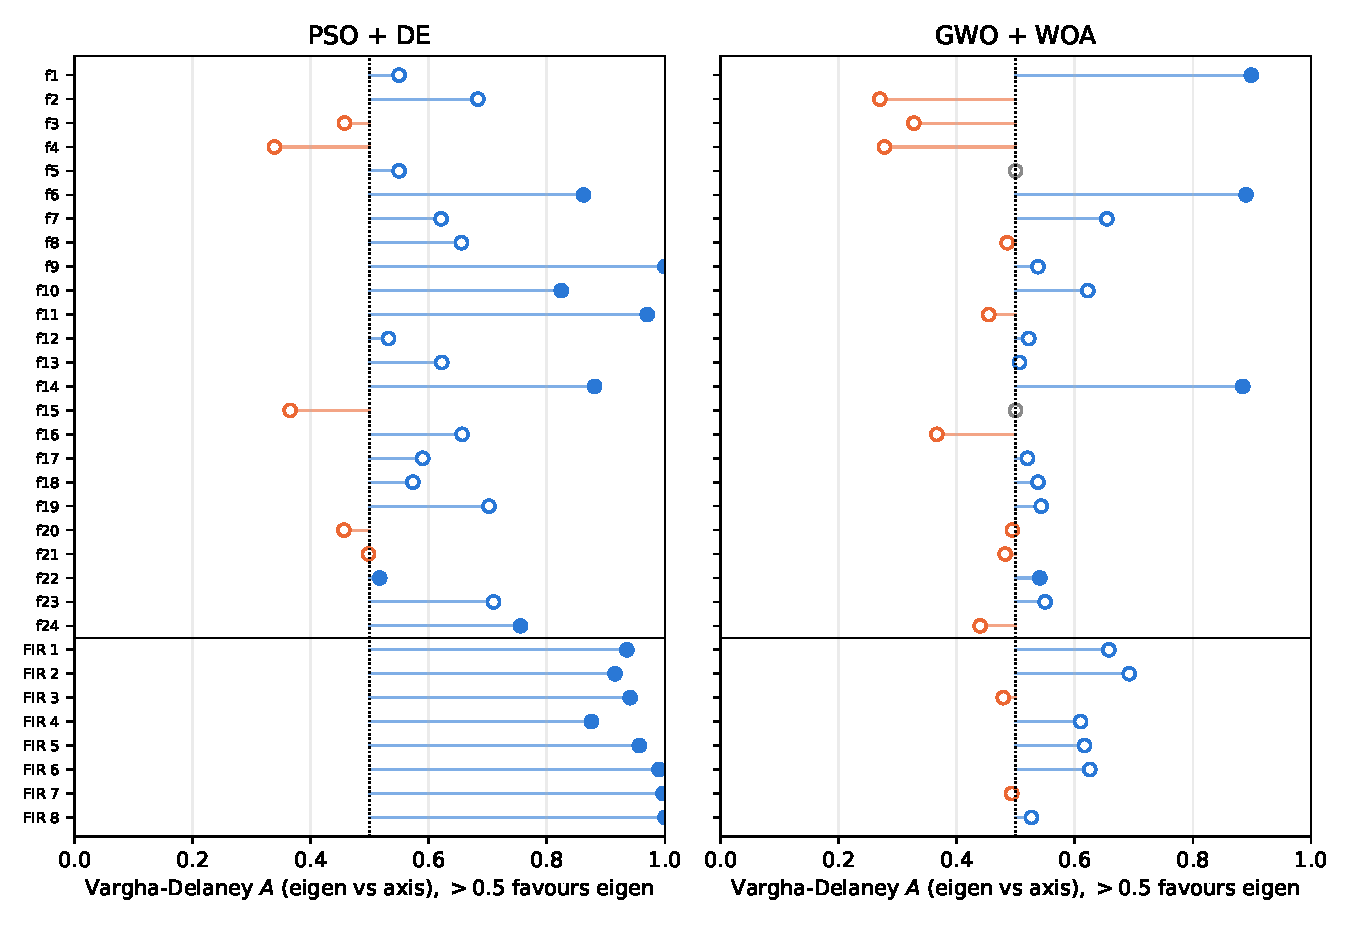
\includegraphics[width=\textwidth]{figures/fig_transfer.pdf}
\caption{Study III: Vargha--Delaney effect $A$ of the eigen-frame arm against its axis-frame twin on the 32 instances for each
parent pair. $A>0.5$ favours the eigen frame (blue); filled markers: significant per-instance paired test (Holm within
benchmark and pair). The horizontal line separates BBOB $D=20$ (top) from FIR.}
\label{fig:transfer}
\end{figure}

\paragraph{PSO with DE} The eigen frame outperforms the axis frame: the median $A$ is \res{X-PD-medA}, better on \res{X-PD-ngt}
and worse on \res{X-PD-nlt} of \res{X-PD-n} instances ($p=\res{X-PD-p}$, $p_\text{Holm}=\res{X-PD-pholm}$), and the result does
not depend on the handling of ties ($p=\res{X-PD-ppratt}$ and \res{X-PD-pzsplit} with Pratt and zero-split handling). It is
significantly better on \res{X-PD-sige} instances and significantly worse on \res{X-PD-siga}: \res{X-PD-B20-sige} of 24 on BBOB
(median $A$ \res{X-PD-B20-medA}) and all \res{X-PD-FIR-sige} of 8 on FIR (median $A$ \res{X-PD-FIR-medA}).

\paragraph{GWO with WOA} The hypothesis is supported, but narrowly and with a small effect: the median $A$ is \res{X-GW-medA},
better on \res{X-GW-ngt}, tied on \res{X-GW-neq} and worse on \res{X-GW-nlt} instances ($p=\res{X-GW-p}$, $p_\text{Holm}=
\res{X-GW-pholm}$; Pratt and zero-split handling give \res{X-GW-ppratt} and \res{X-GW-pzsplit} before Holm). The eigen frame is
significantly better on \res{X-GW-sige} instances, all on BBOB (median $A$ \res{X-GW-B20-medA}), and significantly worse on
none; on FIR the median $A$ is \res{X-GW-FIR-medA} with no significant instance. We read this as a small effect in a
consistent direction, not as a general gain.

\paragraph{Rotation and mechanism} On the rotated ellipsoid f10 the median error falls from \res{X-ell-rot-PDR} to
\res{X-ell-rot-PDE} for PSO with DE and from \res{X-ell-rot-GWR} to \res{X-ell-rot-GWE} for GWO with WOA, while both pairs reach
(PSO+DE) or approach (GWO+WOA) the floor on the separable f2 in either frame, as in Study~II. On rotated Rastrigin f15 the eigen
frame does not help PSO with DE (\res{X-ras-rot-PDE} against \res{X-ras-rot-PDR}) and is on a par for GWO with WOA
(\res{X-ras-rot-GWE} against \res{X-ras-rot-GWR}), and on the separable f3 it is worse for PSO with DE (\res{X-ras-sep-PDE} against \res{X-ras-sep-PDR}), the
same pattern as in Study~II. The acceptance rate of exchanged candidates in the first quarter of the budget does \emph{not}
explain the gain in these pairs: on f10 it is \res{X-acc-PDE-f10}\% for the eigen arm against \res{X-acc-PDR-f10}\% for the axis
arm with PSO and DE, and \res{X-acc-GWE-f10}\% against \res{X-acc-GWR-f10}\% with GWO and WOA, so the higher acceptance seen
for the HBA--MPA hybrid (Study~II) is not a general mechanism. Why the frame helps PSO with DE is therefore not established by
these data.

%% =====================================================================
\section{Discussion}
\label{sec:discussion}

\paragraph{What drives the hybrid} Three components carry the performance of MPHBS on these benchmarks: exchanging
information between the populations at all (decisive on FIR), the amount of exchange per iteration, and the way the
population memory interacts with the mediator. The learned controller and the restructured loop are not among them.
Proposition~\ref{prop:credit} and~\ref{prop:noise} give the main reasons why learning does not help. The table has
$D\cdot N_\mathrm{sub}\cdot 2$ entries (320 on CEC2022, 496 on FIR) and receives $b=\lceil D/5\rceil$ updates per episode,
but by Proposition~\ref{prop:credit} only the provenance of the current vector is updated, so the median updated entry
receives \res{A-th-CEC-median_updates_per_updated_cell} updates on CEC2022 and every entry averages over only about
\res{A-th-memory} of them. The reward is the sign of the change of a whole assembled vector, shared by all $b$ dimensions of
the block, and the evaluated candidate was itself chosen by the proxy score from $K$ candidates generated by different
policies. Finally, the most informative choices, taking coordinates from good members, are already enforced by the ranked
subsets and the rank term of the proxy score~\eqref{eq:proxy}. These properties follow from the update rule and the
reward, not from the algorithm pair; they apply to any mediator of this form.

\paragraph{What carries the exchange} The exchange step is where the populations combine their information, and it was
written for separable problems. Moving it into the eigen frame of the pooled populations makes it invariant to rotations at
no evaluation cost, and Studies~II and~III show that the gain is not specific to one pair: it is large for PSO with DE and the
HBA--MPA hybrid, and small for GWO with WOA, for which these data give no explanation. The
frame helps unimodal or moderately multimodal problems with coupled variables, where the population covariance reflects the
basin; it does not help highly multimodal rotated functions such as f15, and it costs a little on separable multimodal ones
such as f3 and f4. Phase~1 remains coordinate-wise, which is why the gap to CMA-ES, L-SHADE and EA4eig on rotated functions
persists. This is an improvement of a hybrid within its class, not a new state of the art.

\paragraph{Matched controls} The re-evaluating control illustrates two ways in which a control can differ from the learned variant
without anybody intending it: a different number of iterations at the same budget, and a different update of a state
variable. Proposition~\ref{prop:identify} makes the requirement explicit, and Algorithm~\ref{alg:protocol} turns it into a
procedure whose budget and state checks would have exposed both differences before the first run. A paired, seed-matched
design also detects extremely consistent but tiny effects (L4); effect magnitudes should accompany consistency measures.

\paragraph{Practical guidance} For practitioners who use hybrids of this kind, the value table can be replaced by uniform
choices of source and rank without loss, the number of episodes is a more important parameter than the controller, the
treatment of the population memory deserves to be a deliberate decision, and the eigen-frame exchange is a drop-in
replacement with the same budget and a few percent of extra run time. When the choice of algorithm is open, L-SHADE and
CMA-ES remain the stronger default on problems of this size.

\subsection{Limitations}
\begin{itemize}
\item \emph{Scope.} Study~I covers one hybrid in its reference configurations, selected with SARSA on CEC2022 and FIR,
which makes L1 conservative; Studies~II and~III cover problems with $D\le31$. The confirmatory effect in Study~II is small and
sensitive to the handling of tied instances. No free lunch results~\citep{wolpert1997nfl} caution against generalising beyond the
problems studied.
\item \emph{Transfer.} Study~III covers two further pairs on two benchmark families with the mediator settings of the
reference hybrid; the effect for GWO with WOA is small, and the mechanism of the gain for PSO with DE is not identified.
\item \emph{Choices fixed by pilot.} The value $q=0.5$ was chosen from a pilot with two values; other values or an adaptive
$q$ may perform differently. The classical algorithms were added after the main analysis of Study~II and use standard, not
tuned, settings. The EA4eig comparison is unpaired and across implementations; run times were measured on a shared laptop.
\item \emph{Port and platform.} Study~I uses a Python port whose agreement with the reference MATLAB implementation is
distributional, because random streams differ.
\item \emph{Exploratory parts.} L5--L8, the theory check and the BBOB extension are exploratory and should be confirmed
independently. The relative difference $\hat\delta$ was added after the pre-registration.
\item \emph{Dimension.} For larger $D$ the $O(D^3)$ decomposition and the reliability of the covariance estimate from $2N$
points should be checked.
\end{itemize}

%% =====================================================================
\section{Conclusion}
\label{sec:conclusion}
A contrast between a learned component and a control mixes learning, budget and state effects unless the control is matched,
and ablations of learned components in metaheuristics should therefore be budget- and state-matched, verified mechanically,
fixed in advance and reported with effect magnitudes. In the hybrid studied here, random choices are as effective as the
learned controller at an equal budget; the update rule explains why, because it credits each reward to the provenance of the
current vector and its learning rate limits each entry to an average over about \res{A-th-memory} updates, and logged runs
confirm both effects. The exchange step carries the performance, and making it independent of the coordinate system, by
recombining in the eigenvector frame of the pooled populations, improves the hybrid without extra evaluations: in
\res{E-runs-total} runs on CEC2022, BBOB and FIR it was never significantly worse than the original and reduced the median
error on the rotated ellipsoid \res{E-f10-ratio-MPHBS}-fold. In a pre-registered study of \res{X-runs} runs the same exchange
helps two other parent pairs, strongly for PSO with DE and slightly for GWO with WOA. The remaining gap to CMA-ES, L-SHADE and
EA4eig, the failure on rotated multimodal functions and the missing mechanism for the transfer are the natural next steps,
together with an adaptive frame probability and rotation-invariant native moves.

\FloatBarrier
\section*{Statements and Declarations}
\paragraph{Competing interests} The author has no competing interests to declare that are relevant to the content of this article.
\paragraph{Funding} No funding was received for conducting this study.
\paragraph{Data and code availability} The repository \url{https://github.com/abinaya-g/la-kaie} holds the code, the frozen
pre-registrations and design documents (Study~I: tag \texttt{pathA-prereg-frozen} and the BBOB addendum, tag
\texttt{pathA-bbob-run-1}; Studies~II and~III: \path{experiments/ESWA_EIGEN_CAMPAIGN.md}, Sections 1--10), the record of every
run (final error, evaluations, run time, configuration and seed), the analyses and the scripts from which each number, table
and figure of this paper is produced (\path{scripts/combined_assets.py}). The official EA4eig results are redistributed with
their source in \path{data/external/cec2022_ea4eig/}.
\paragraph{Author contributions} Abinaya G conceived and designed the study, wrote the software, ran the experiments and the
analysis, and wrote the manuscript.


\FloatBarrier
\bibliographystyle{plainnat}
\bibliography{refs}

\end{document}
